\chapter{Evaluation}

\section{Customer Requirements}

\subsection{General Objective Evaluation}

\subsubsection{-Data can added to the database easily}
\textbf{Was the Objective Fulfilled?} \newline

\textbf{\large{This objective has been fulfilled successfully.}}

The data fields have been labelled so that the user knows what data they need to enter into the field. Evidence for this can be in figure \ref{fig:evaluation-1} in the Evidence Section. The information in which the user must enter has been grouped together in a group box, for the convenience of the user, which is evidenced in figure \ref{fig:evaluation-2}, figure \ref{fig:evaluation-3} and figure \ref{fig:evaluation-4} in the Evidence section.


The system clearly shows when the user has entered valid or non valid data by creating a green border around each data field. Evidence for the current validation for my system can be found in figure \ref{fig:evaluation-5}.

Adding a Product Employee and a Member are all done in a similar fashion which reduces the time having to learn how to add each aspect to the system. The system will clearly state whether the product, member or employee has been added successfully or not, with a pop up window telling them.\newline

\pagebreak
\textbf{Evidence} \newline

\begin{figure}[H]
\caption{Evidence for data field labels} \label{fig:evaluation-1}
\hfill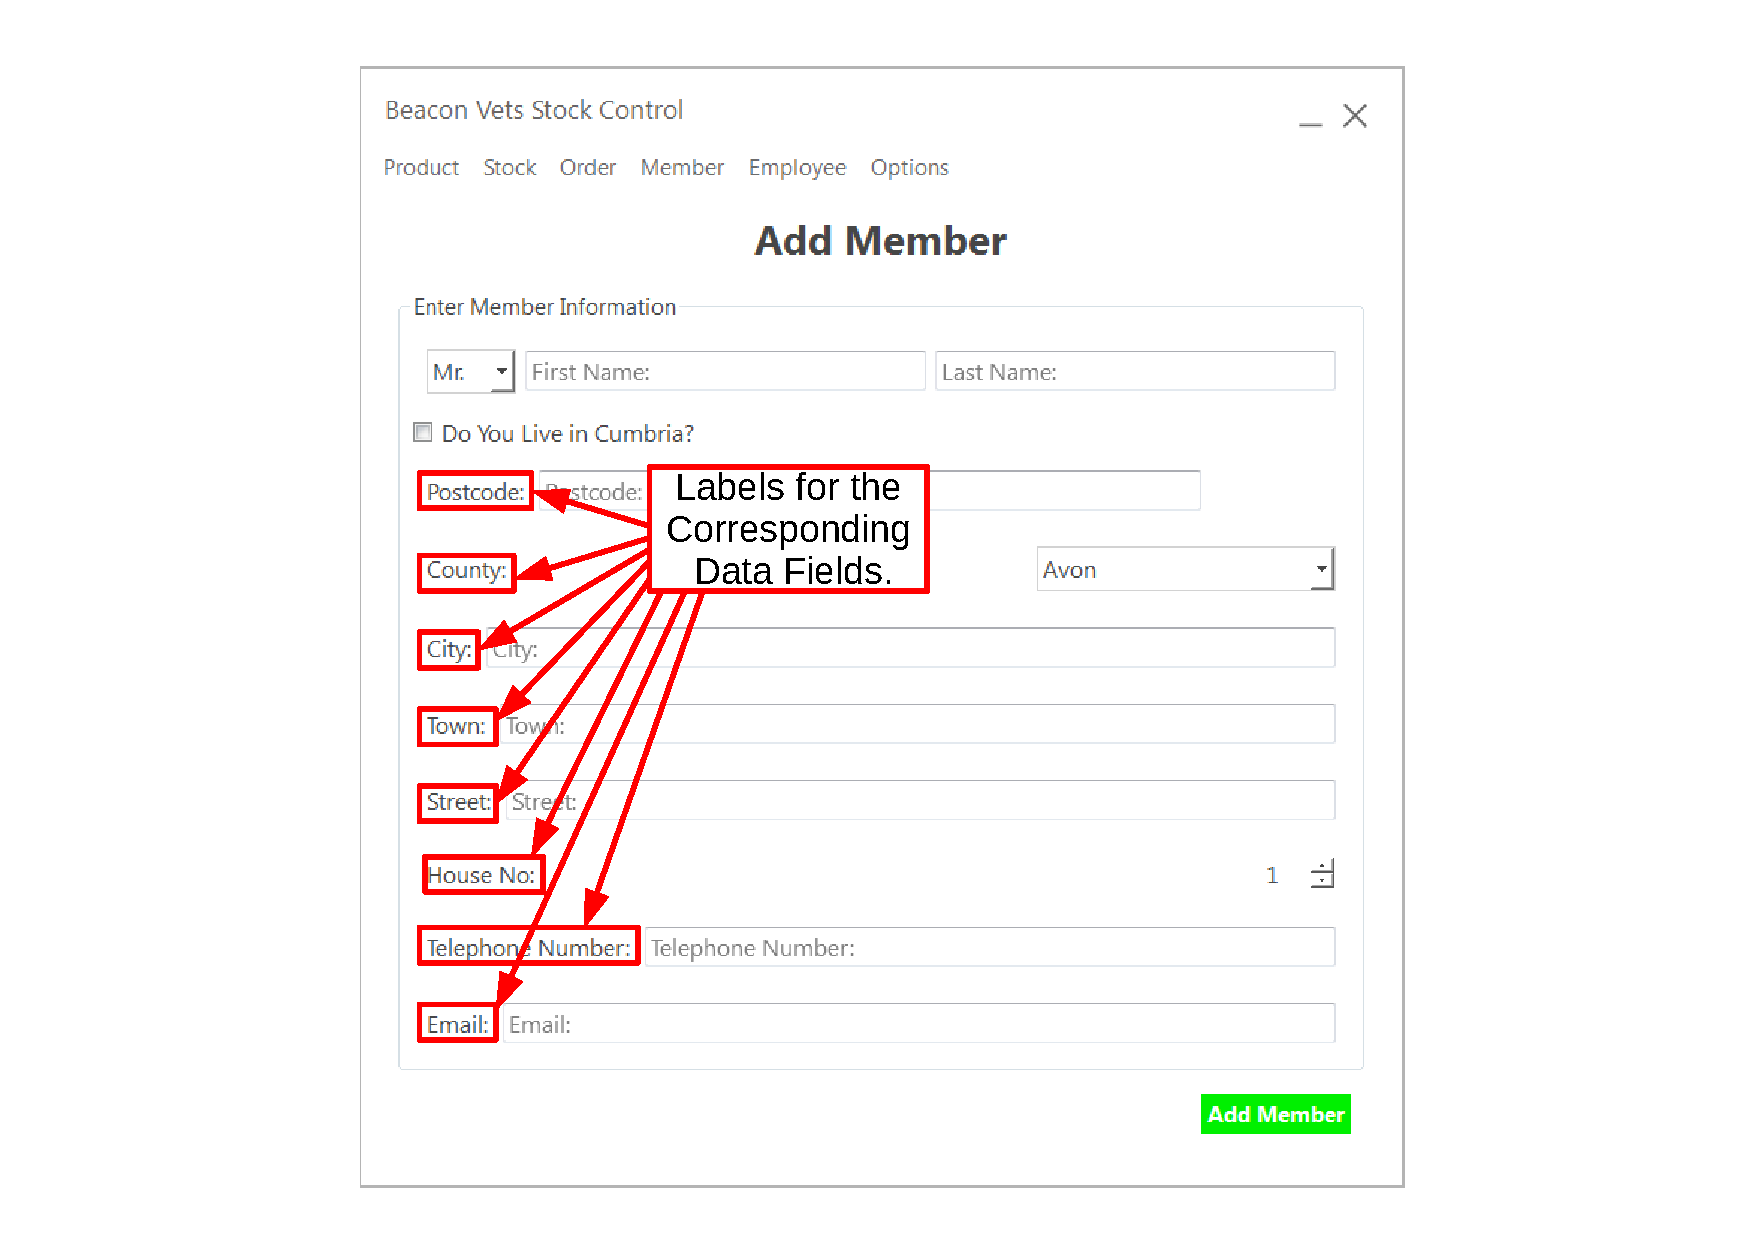
\includegraphics[width = \textwidth]{./Evaluationimages/evaluation-1.pdf}
\end{figure}

\begin{figure}[H]
\caption{Evidence for data inputs being grouped in a Group Box.} \label{fig:evaluation-2}
\hfill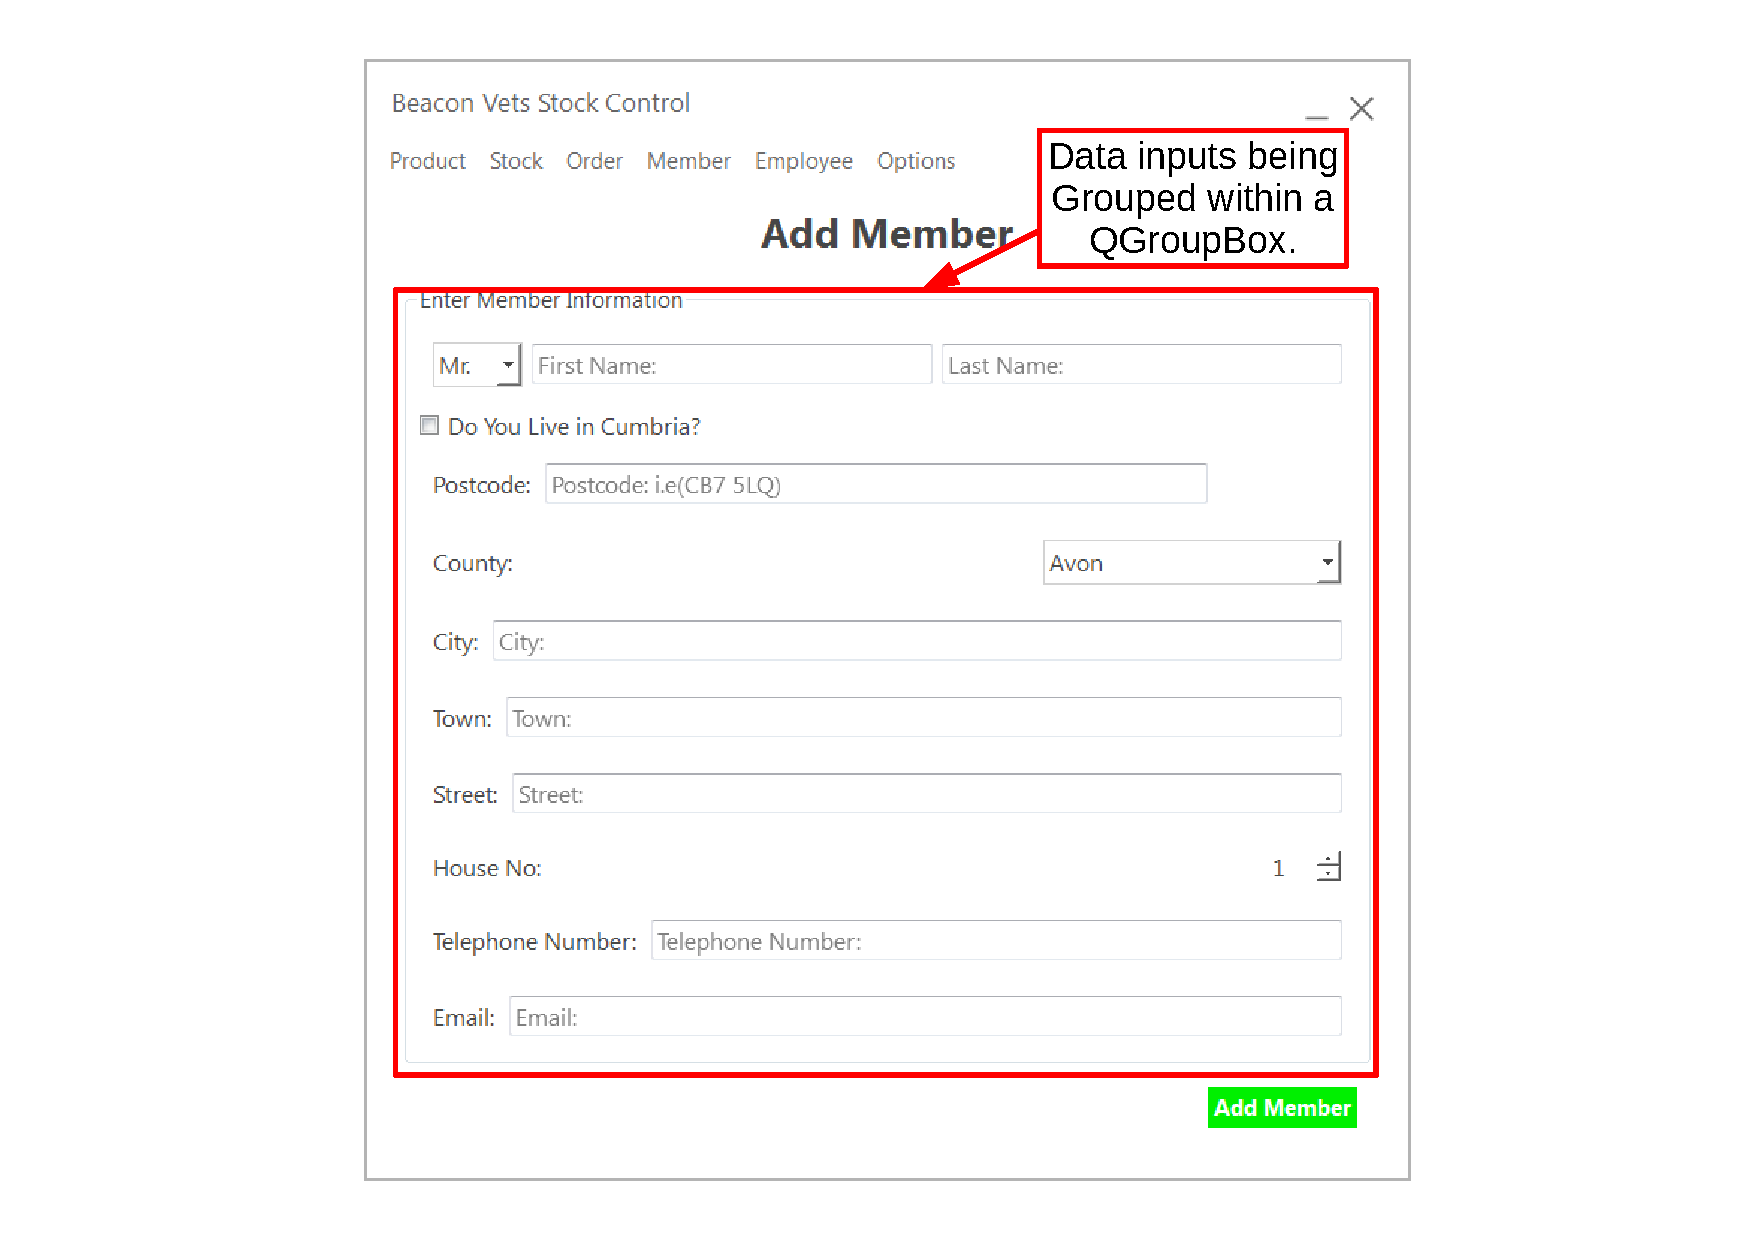
\includegraphics[width = \textwidth]{./Evaluationimages/evaluation-2.pdf}
\end{figure}

\begin{figure}[H]
\caption{Evidence for data inputs being grouped in a Group Box.} \label{fig:evaluation-3}
\hfill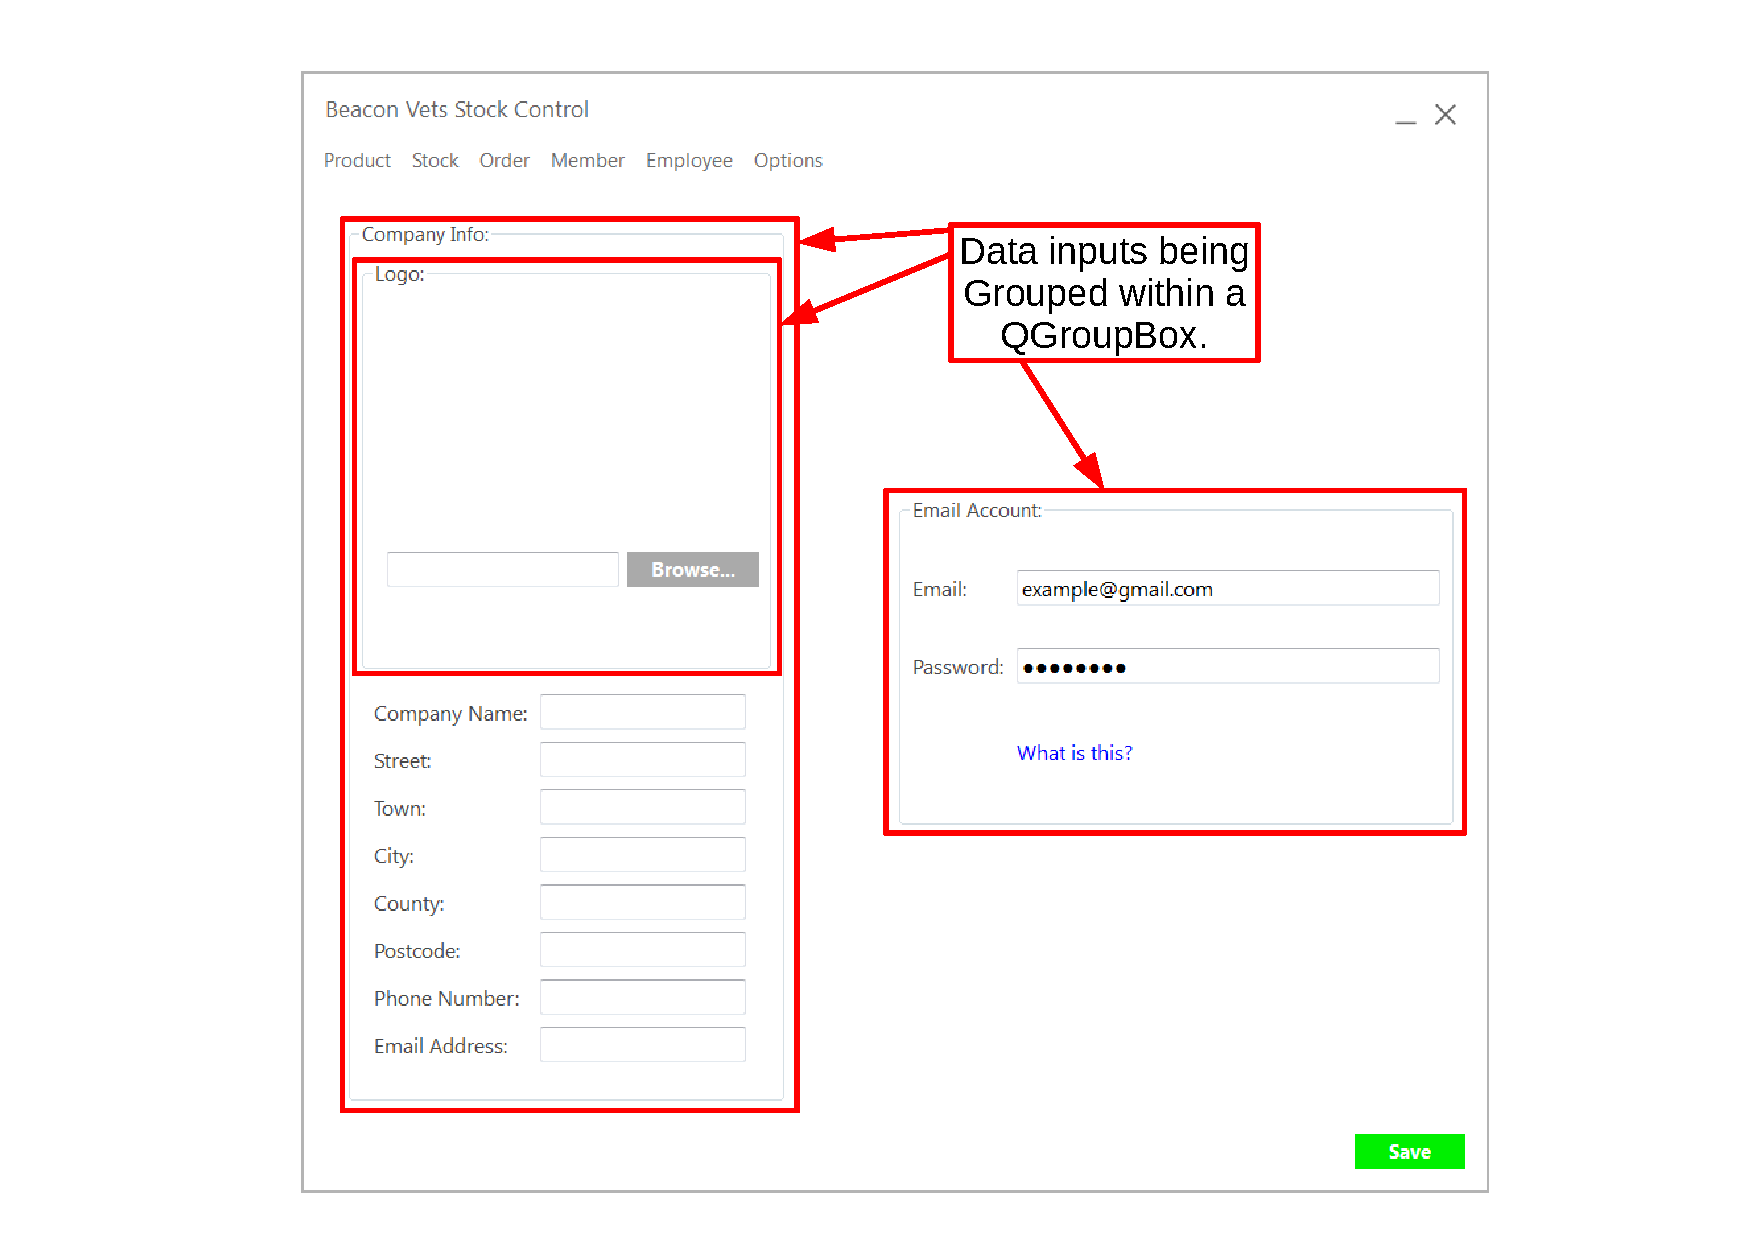
\includegraphics[width = \textwidth]{./Evaluationimages/evaluation-3.pdf}
\end{figure}

\begin{figure}[H]
\caption{Evidence for data inputs being grouped in a Group Box.} \label{fig:evaluation-4}
\hfill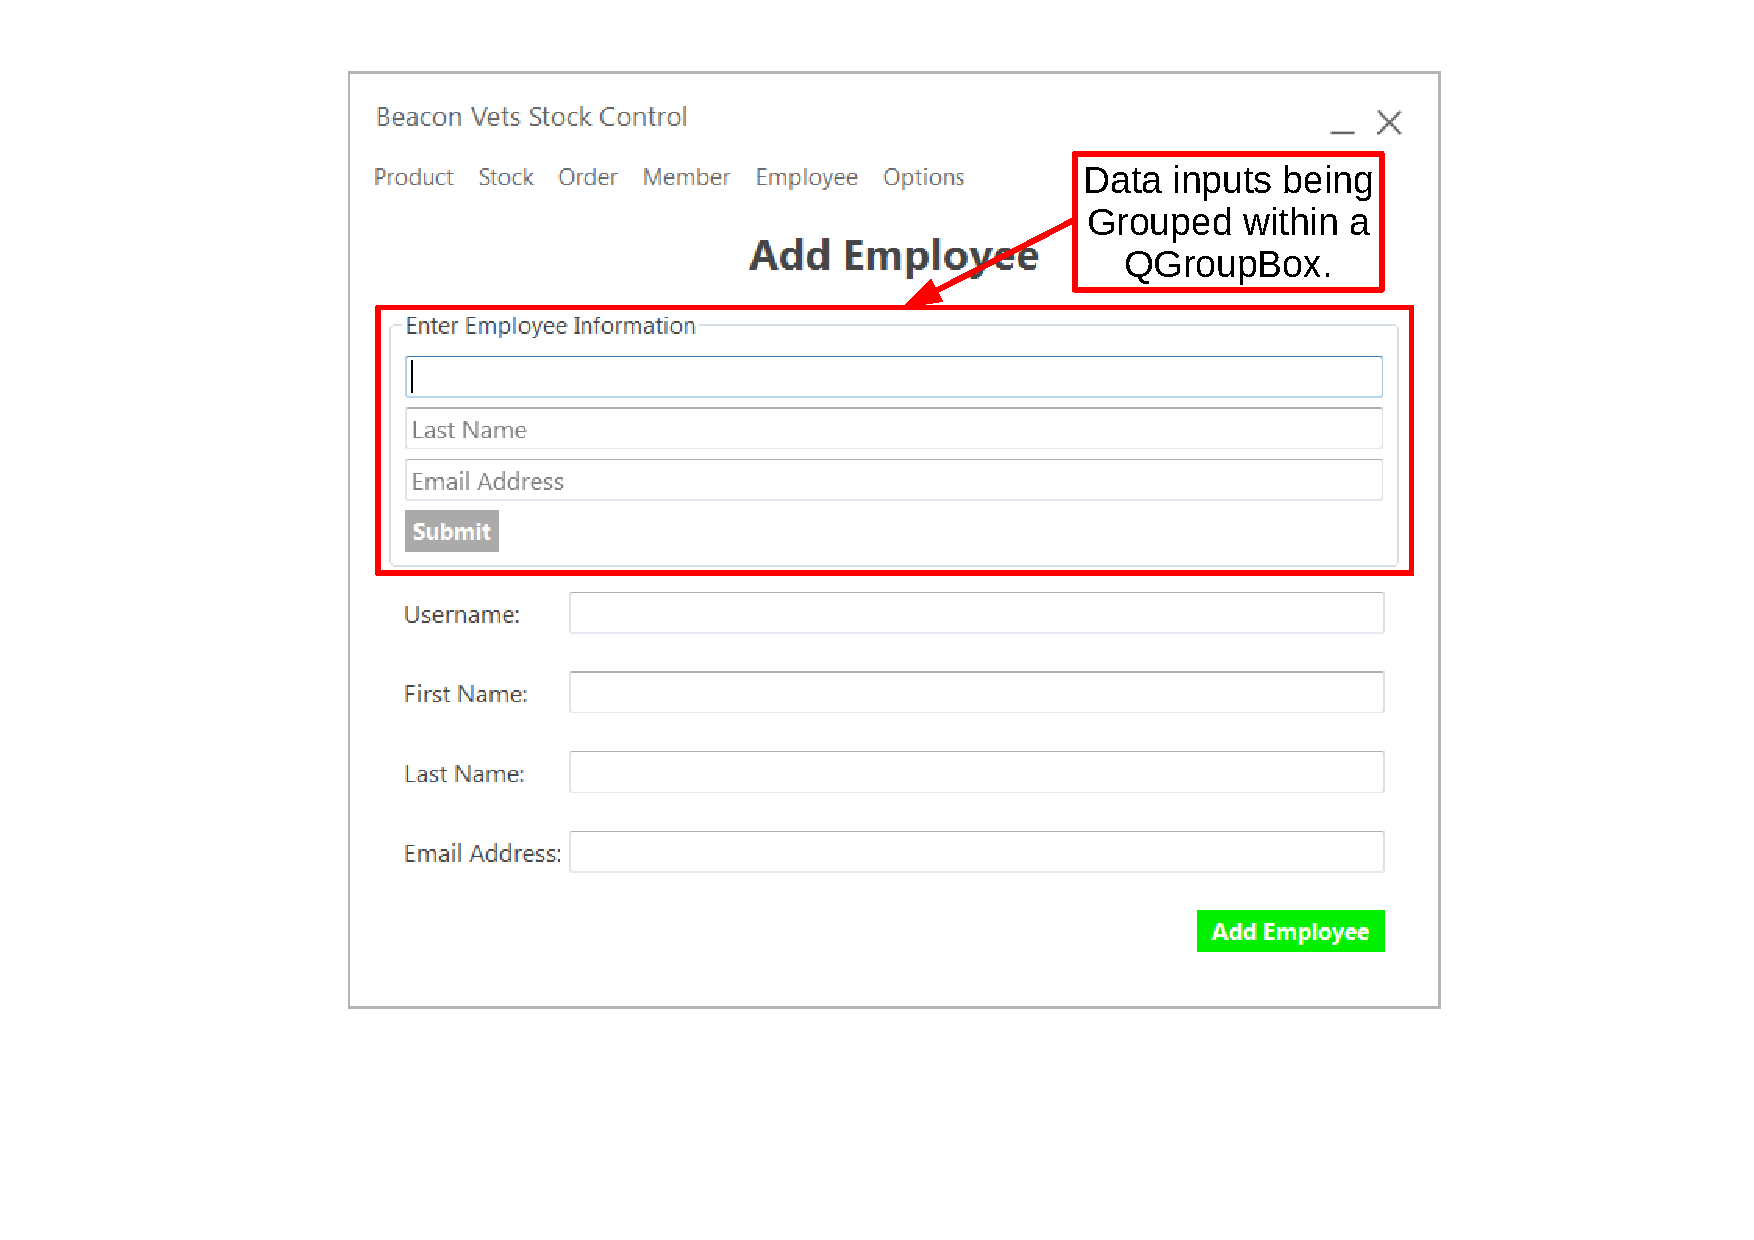
\includegraphics[width = \textwidth]{./Evaluationimages/evaluation-4.pdf}
\end{figure}

\begin{figure}[H]
\caption{Evidence for data Validation on data input fields.} \label{fig:evaluation-5}
\hfill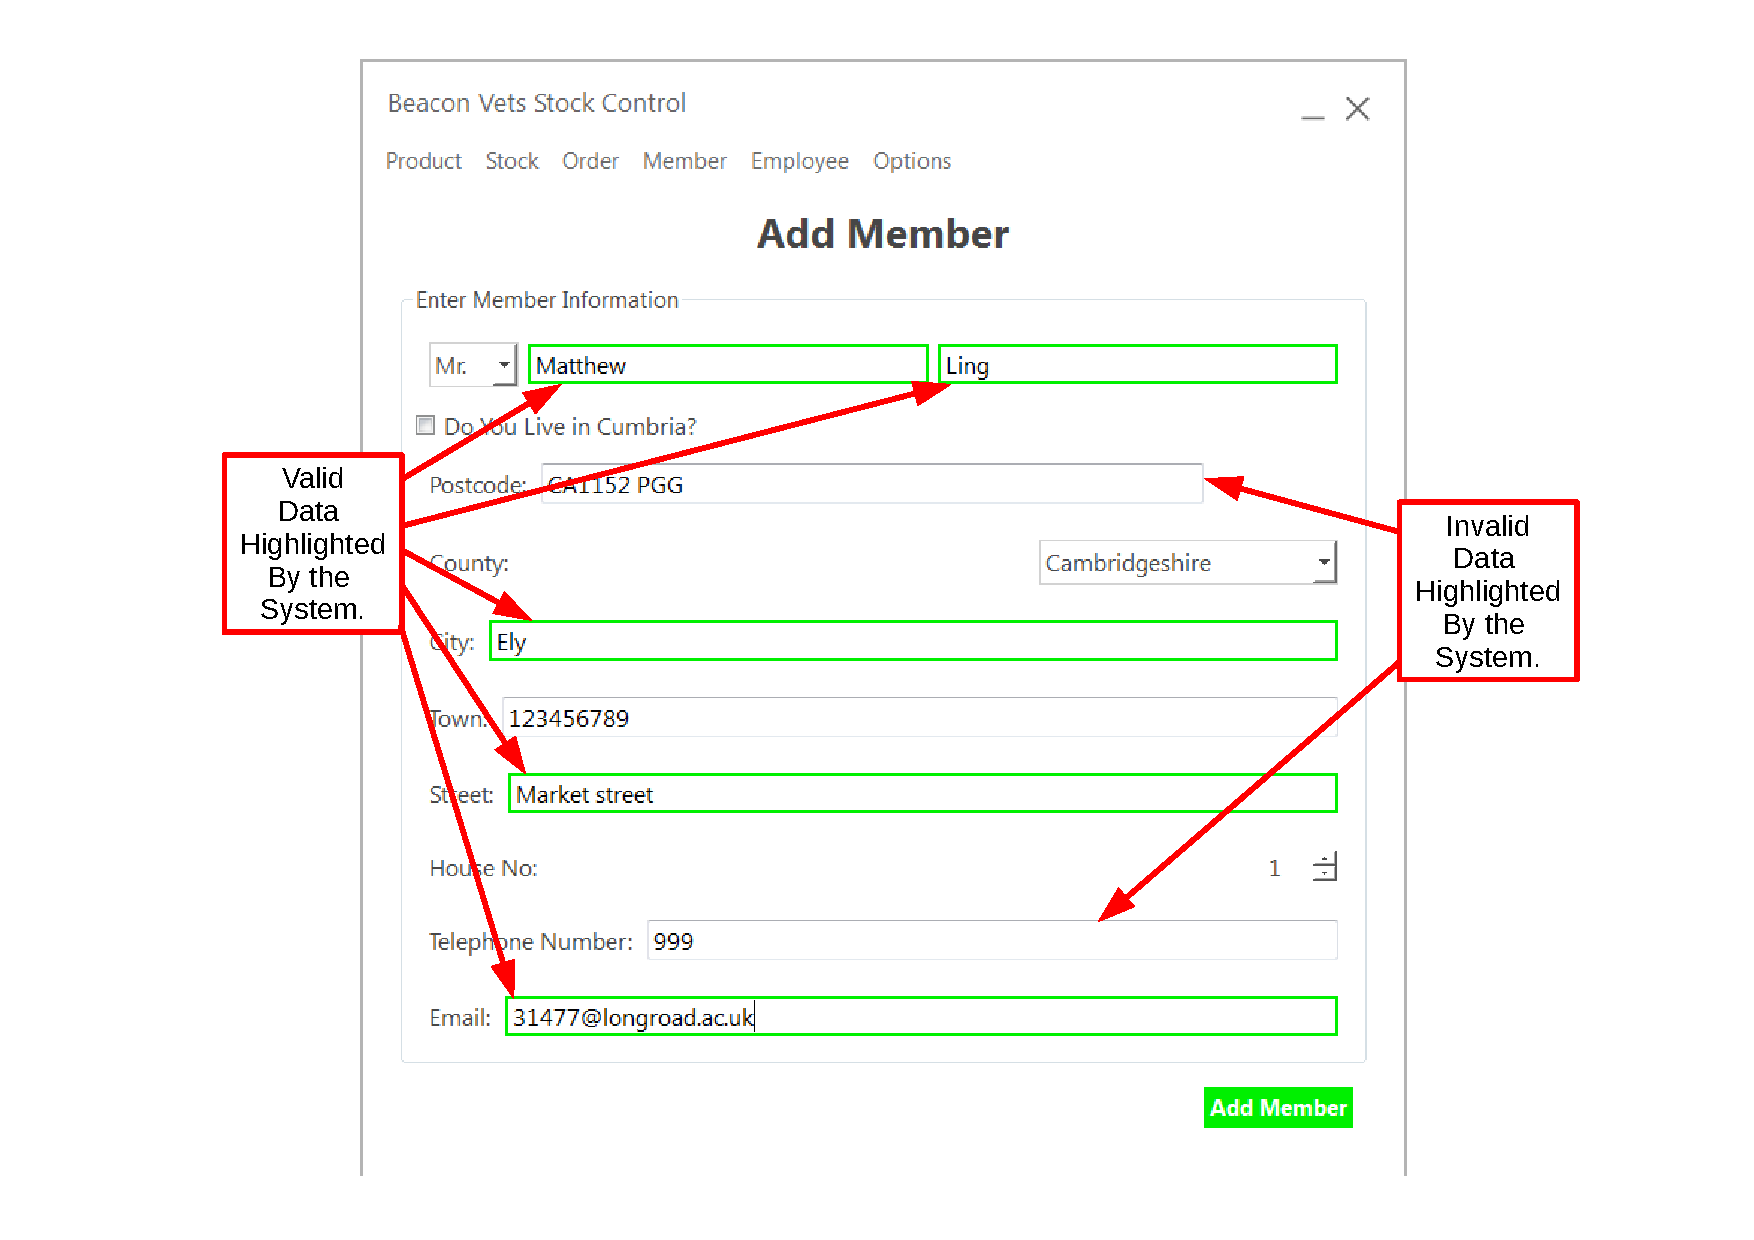
\includegraphics[width = \textwidth]{./Evaluationimages/evaluation-5.pdf}
\end{figure}

\pagebreak

Figure \ref{graph1} Shows a bar chart, displaying the results for Question 1 of my questionnaire.

\begin{figure}[H]
\caption{A Bar Chart displaying the responses from the 7 users from Question 1 of my questionnaire} \label{graph1}
\hfill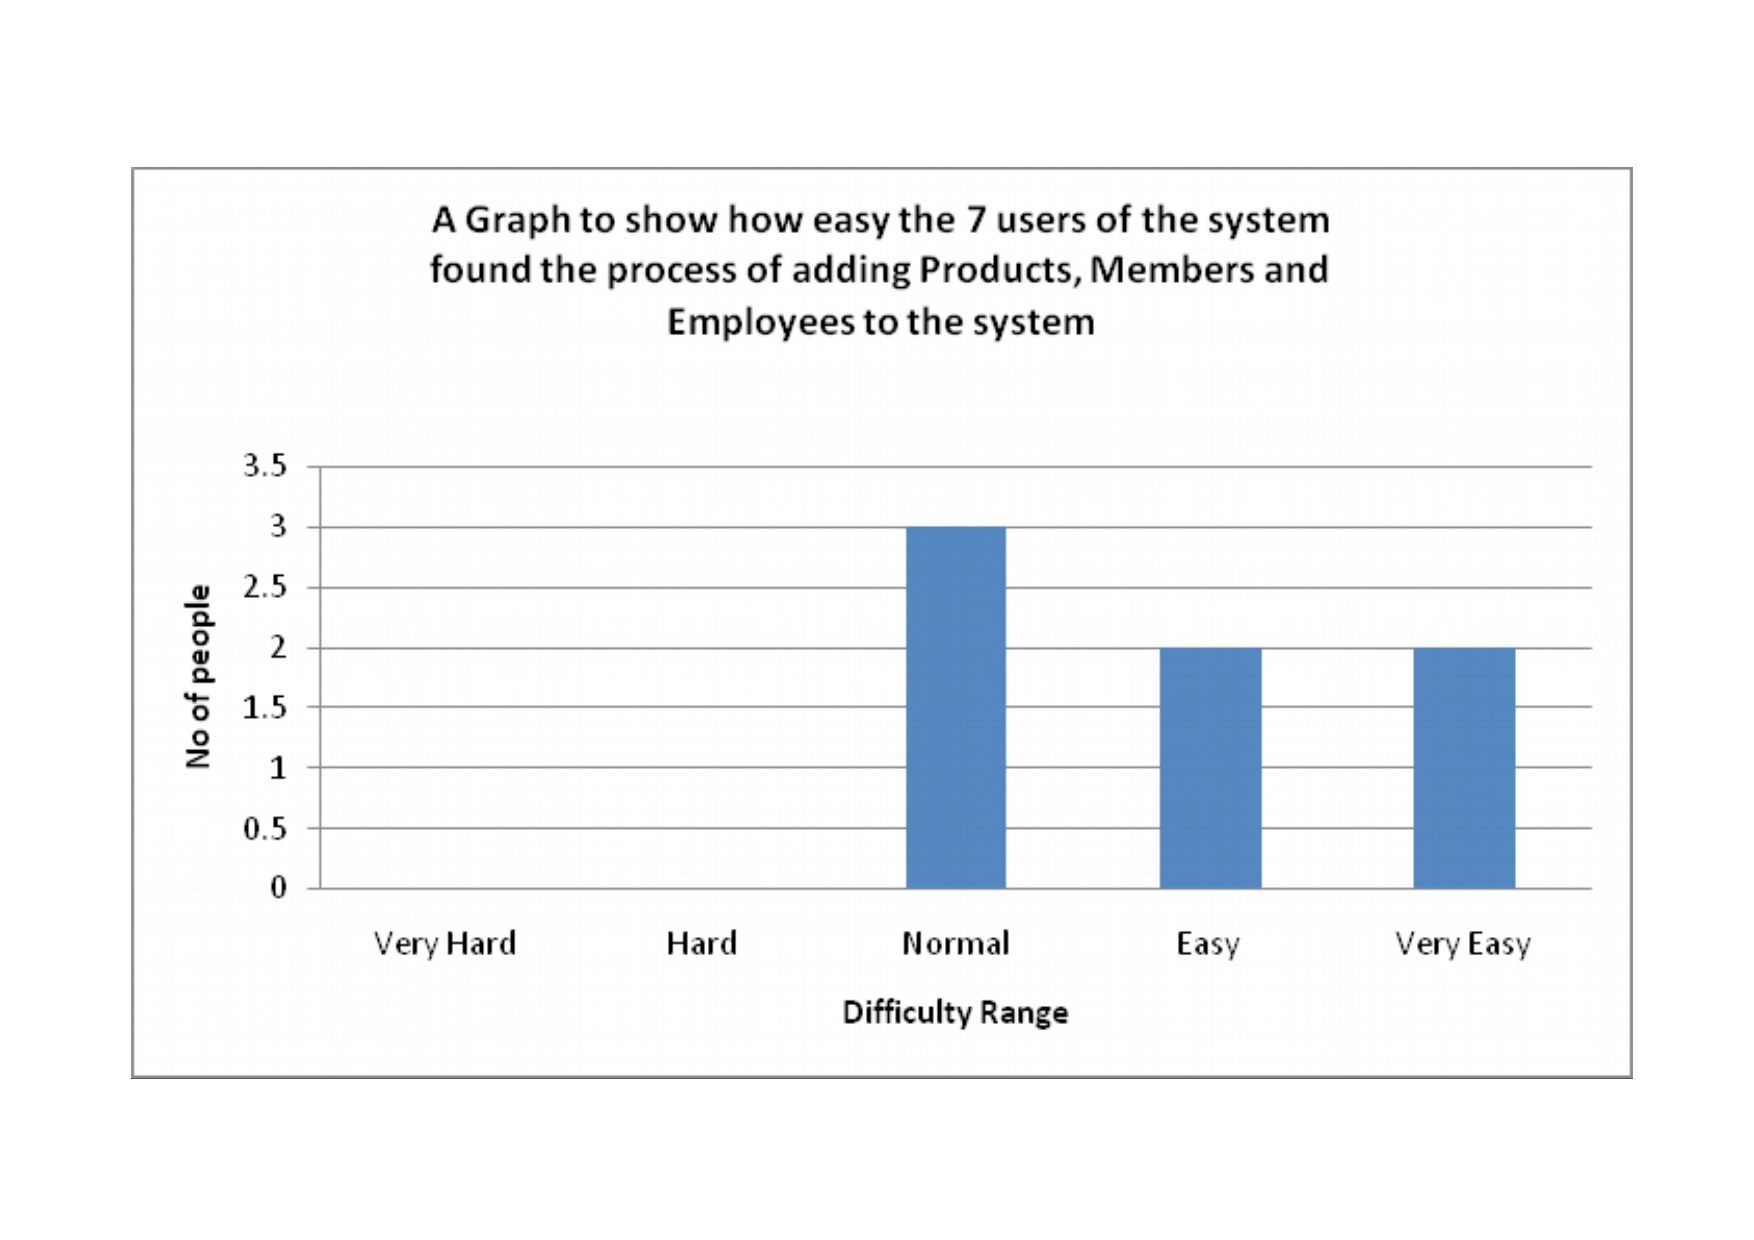
\includegraphics[width = \textwidth]{./Evaluationimages/graph1.pdf}
\end{figure}

From the graph, i can see that 4 out of the 7 users found the process of adding data either easy or very easy. None of the users found the process hard or very hard, which provides evidence that this objective has been fulfilled.





\pagebreak
\subsubsection{-Data can be edited within the system easily.}
\textbf{Was the Objective Fulfilled?} \newline

\textbf{\large{This objective has been fulfilled successfully.}}

  The user has to enter the ID of the item they would like to edit, and the edit interface will allow them to change the data. As specified above, the data inputs have been grouped together which is convenient for the user, the edit interface also has a clear edit button in the bottom right hand corner of the interface in which the user can click when they have finished editing the information. The button is bright green which means it is obvious for the user to see. This is evidenced in figure \ref{fig:evaluation-6} in the Evidence section.\newline

\textbf{Evidence} \newline

\begin{figure}[H]
\caption{Evidence that data can be edited easily.} \label{fig:evaluation-6}
\hfill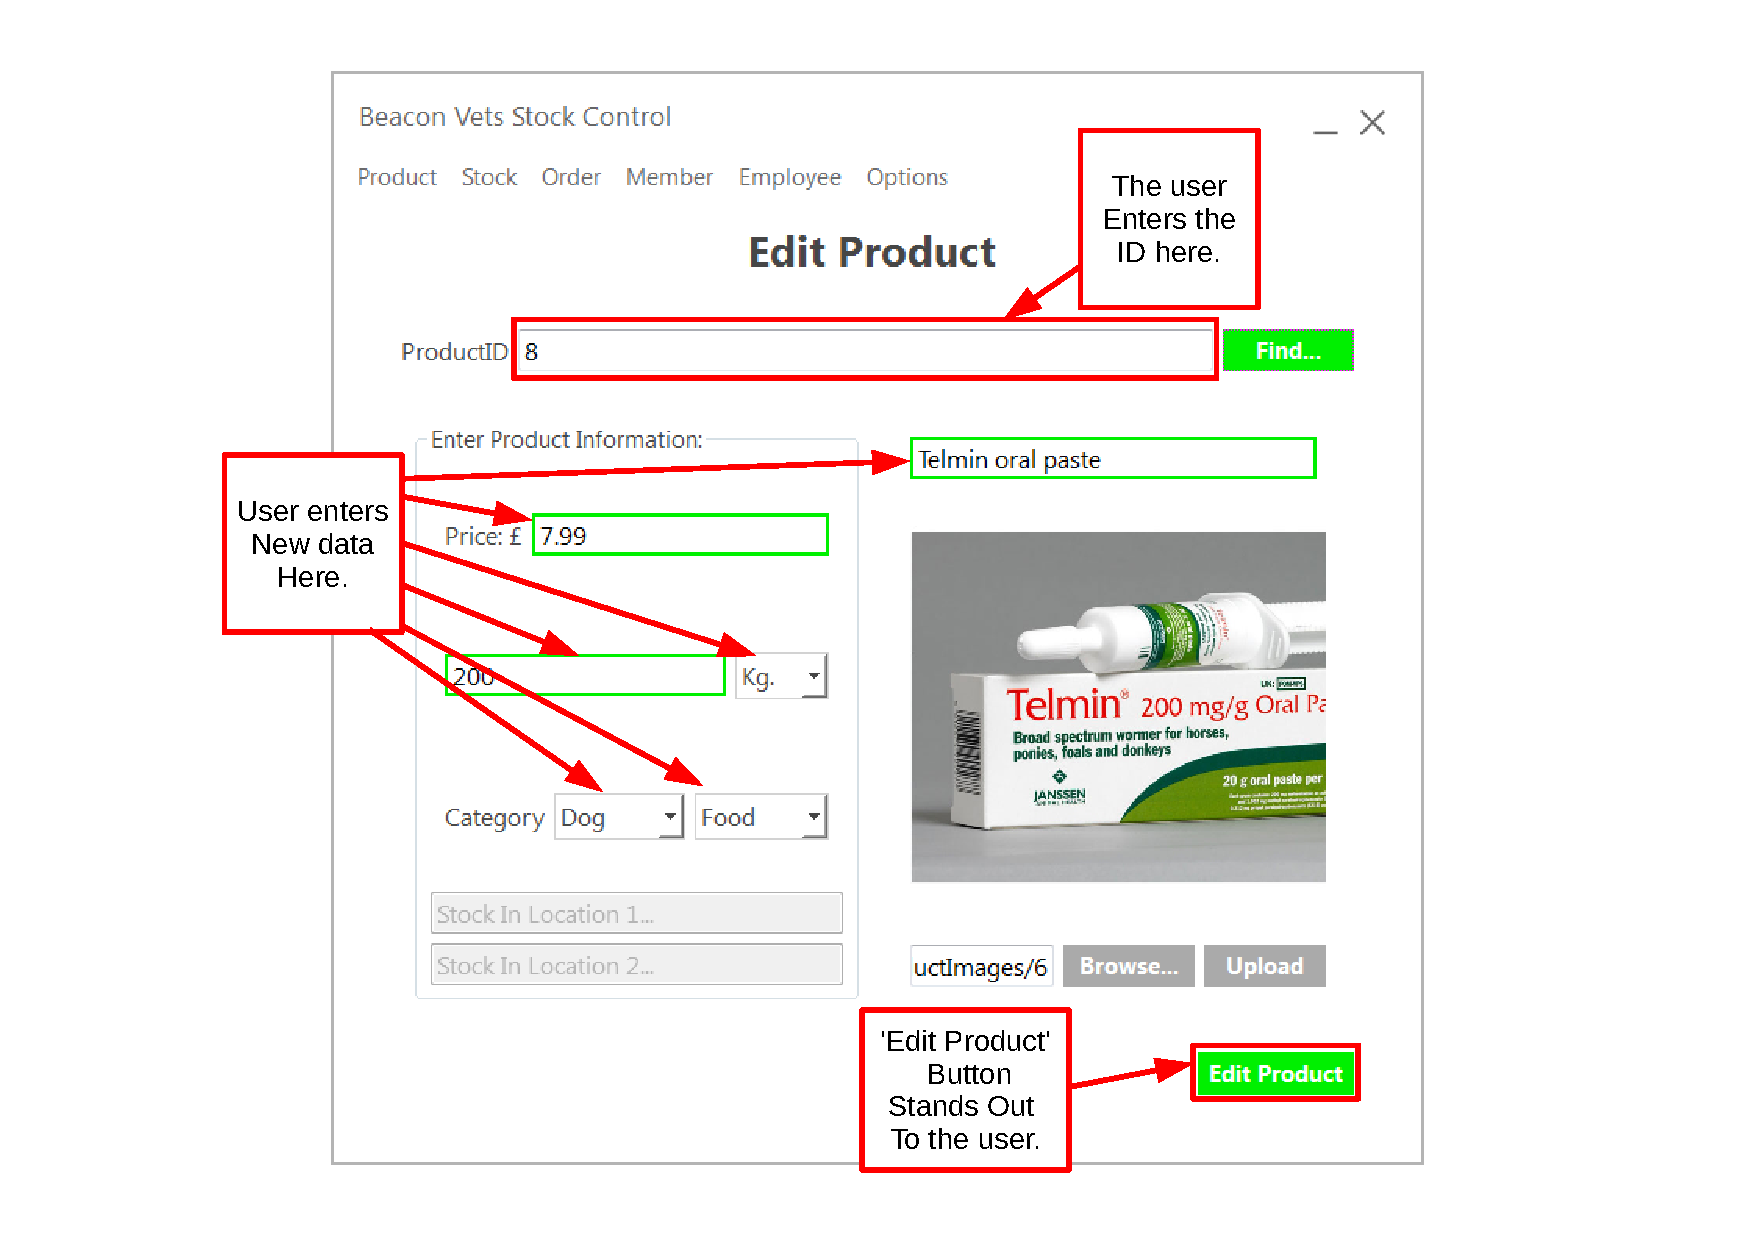
\includegraphics[width = \textwidth]{./Evaluationimages/evaluation-6.pdf}
\end{figure}

Figure \ref{graph2} below, shows how easy or hard the 7 users found the process of editing data in the system. This was asked in Question 2 of the questionnaire.

\begin{figure}[H]
\caption{A Bar chart to display the response from Question 2 of my questionnaire} \label{graph2}
\hfill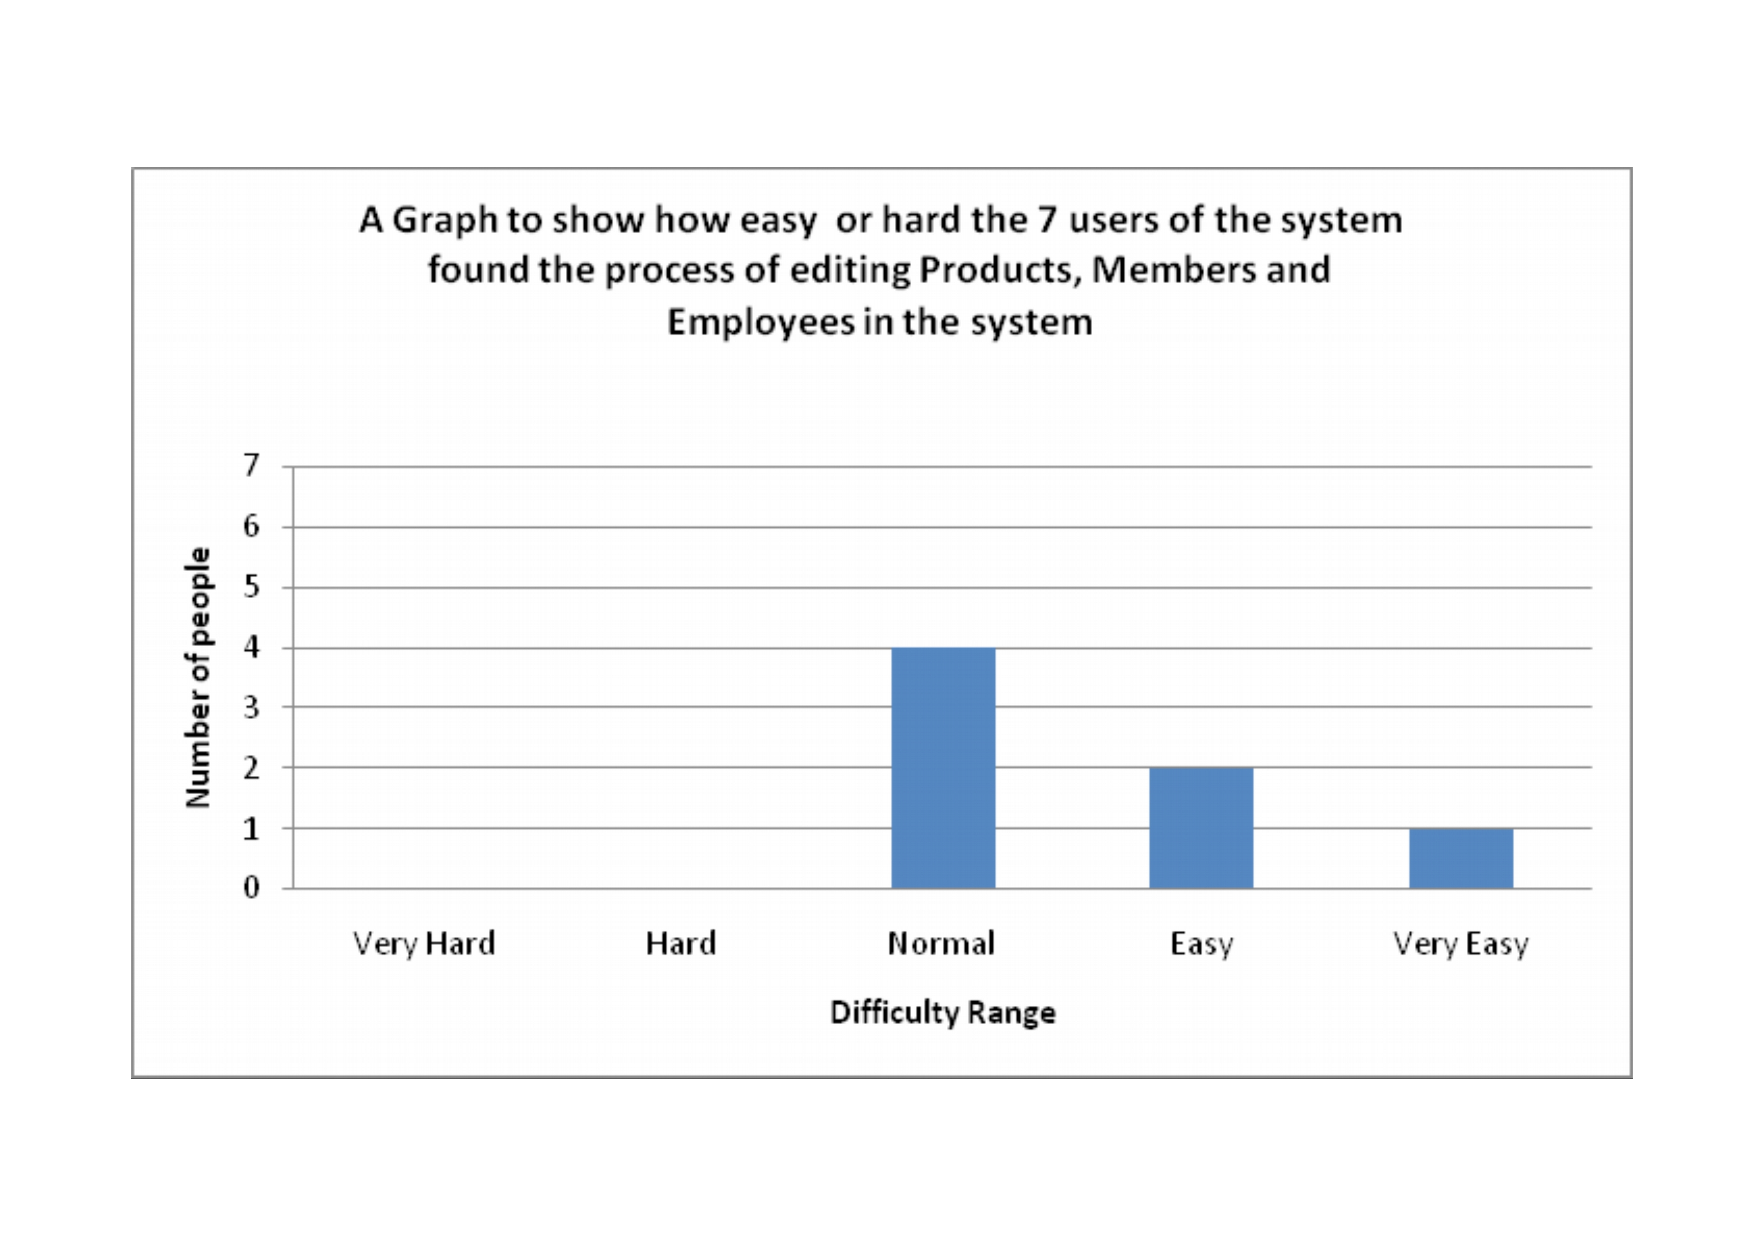
\includegraphics[width = \textwidth]{./Evaluationimages/graph2.pdf}
\end{figure}

Looking at Figure \ref{graph2}, 3 out of the 7 users felt that editing data was either easy or very easy. This shows that the users, in general, found it harder to edit the data compared to adding it. This was concluded by comparing the amount of people that felt the process was either easy or very easy between Figure \ref{graph1} on page \pageref{graph1} and Figure \ref{graph2} above.

0 out of the 7 users found the process of editing data hard or very hard which can conclude that this objective has been fulfilled.




\pagebreak
\subsubsection{-Easy to understand the layout of the information.}
\textbf{Was the Objective Fulfilled?} \newline

\textbf{\large{This objective was fulfilled successfully}}

Information was placed in group boxes where possible to organise the information displayed to the user. data input and output fields were also designed to be similar to other programs in which the users may have used to reduce the learning curve of the system. 


\textbf{Evidence} \newline

Evidence that making the data inputs and outputs similar to other programs was useful, is my clients reply to Question 1 which can be found on page \pageref{Client-Q1}. A word processed version of the response has been provided in figure \ref{client-evidence-Q1} below. \newline

\begin{figure}[H]
\caption{Word Processed version of my clients response to question 1 in the questionnaire} \label{client-evidence-Q1}
\vspace{3mm}
\textit{\large{"I was able to do this without help because it was similar to other programs. I agree that this objective has been met."}}
\vspace{3mm}
\end{figure}

This response provides evidence that the data fields displaying the information have been organised in such a fashion, that they are similar to other programs. My client was able to add a product to the system without any given instructions because the layout of the data fields was well structured, which concludes this objective has been fulfilled.



\pagebreak
\subsubsection{-Easy to locate a product within the system.}
\textbf{Was the Objective Fulfilled?} \newline

\textbf{\large{This objective was fulfilled successfully}}

To locate a product within the system, the user can use the search window. There are multiple ways to access the search window, which decreases the difficulty of accessing it. The structure of the search window is easy to understand and the user can search for data by entering keywords into the search field and the system will return the search results instantly. The results of the search can be re-ordered by clicking on the column headings. This is evidenced on page \pageref{}. The keywords can match any data that is display in the product table, be it the ProductID, ProductName, Price Category.\newline

\textbf{Evidence} \newline

\begin{figure}[H]
\caption{Evidence that searching for data within the system can be done easily.} \label{fig:evaluation-7}
\hfill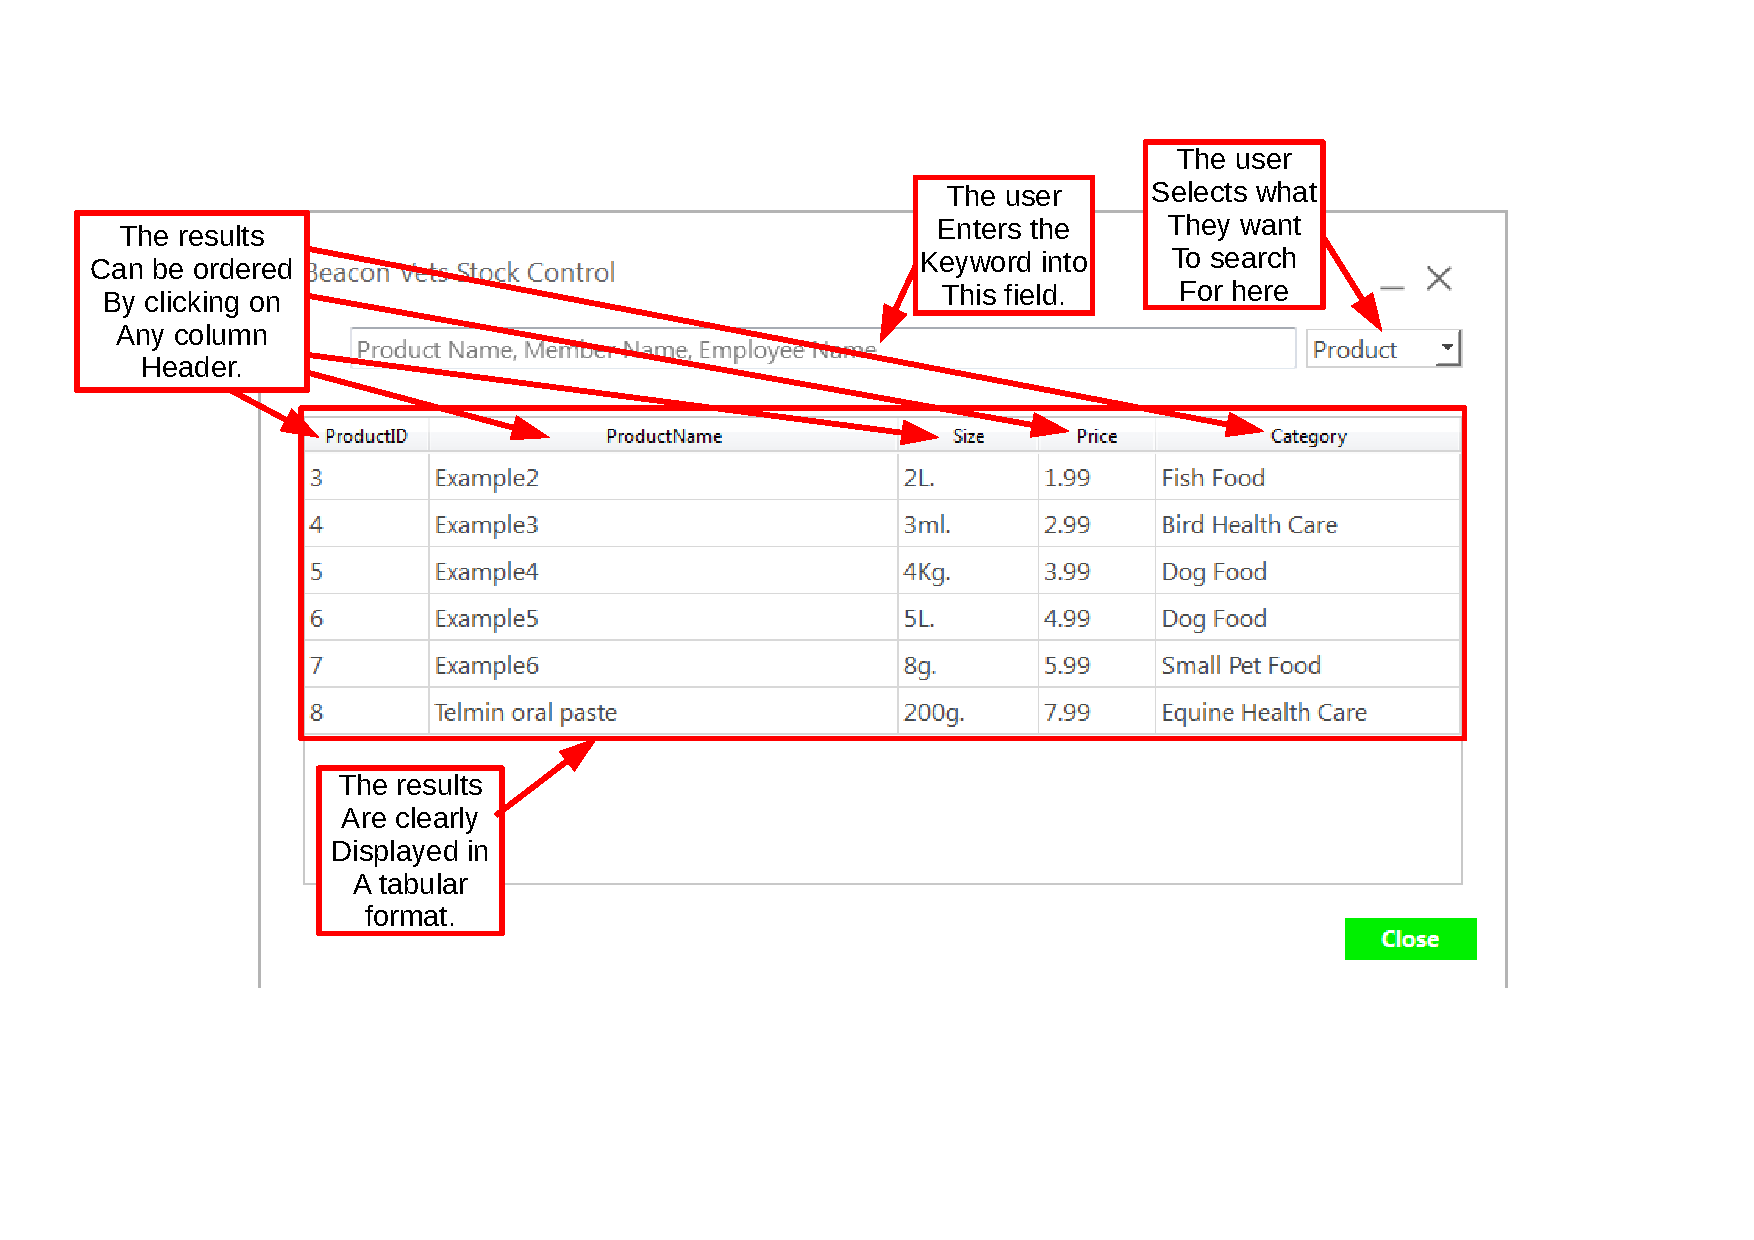
\includegraphics[width = \textwidth]{./Evaluationimages/evaluation-7.pdf}
\end{figure}

\pagebreak

Figure \ref{graph3} shows the responses from the seven users from Question 3 of the questionnaire.

\begin{figure}[H]
\caption{Evidence that searching for data within the system can be done easily.} \label{graph3}
\hfill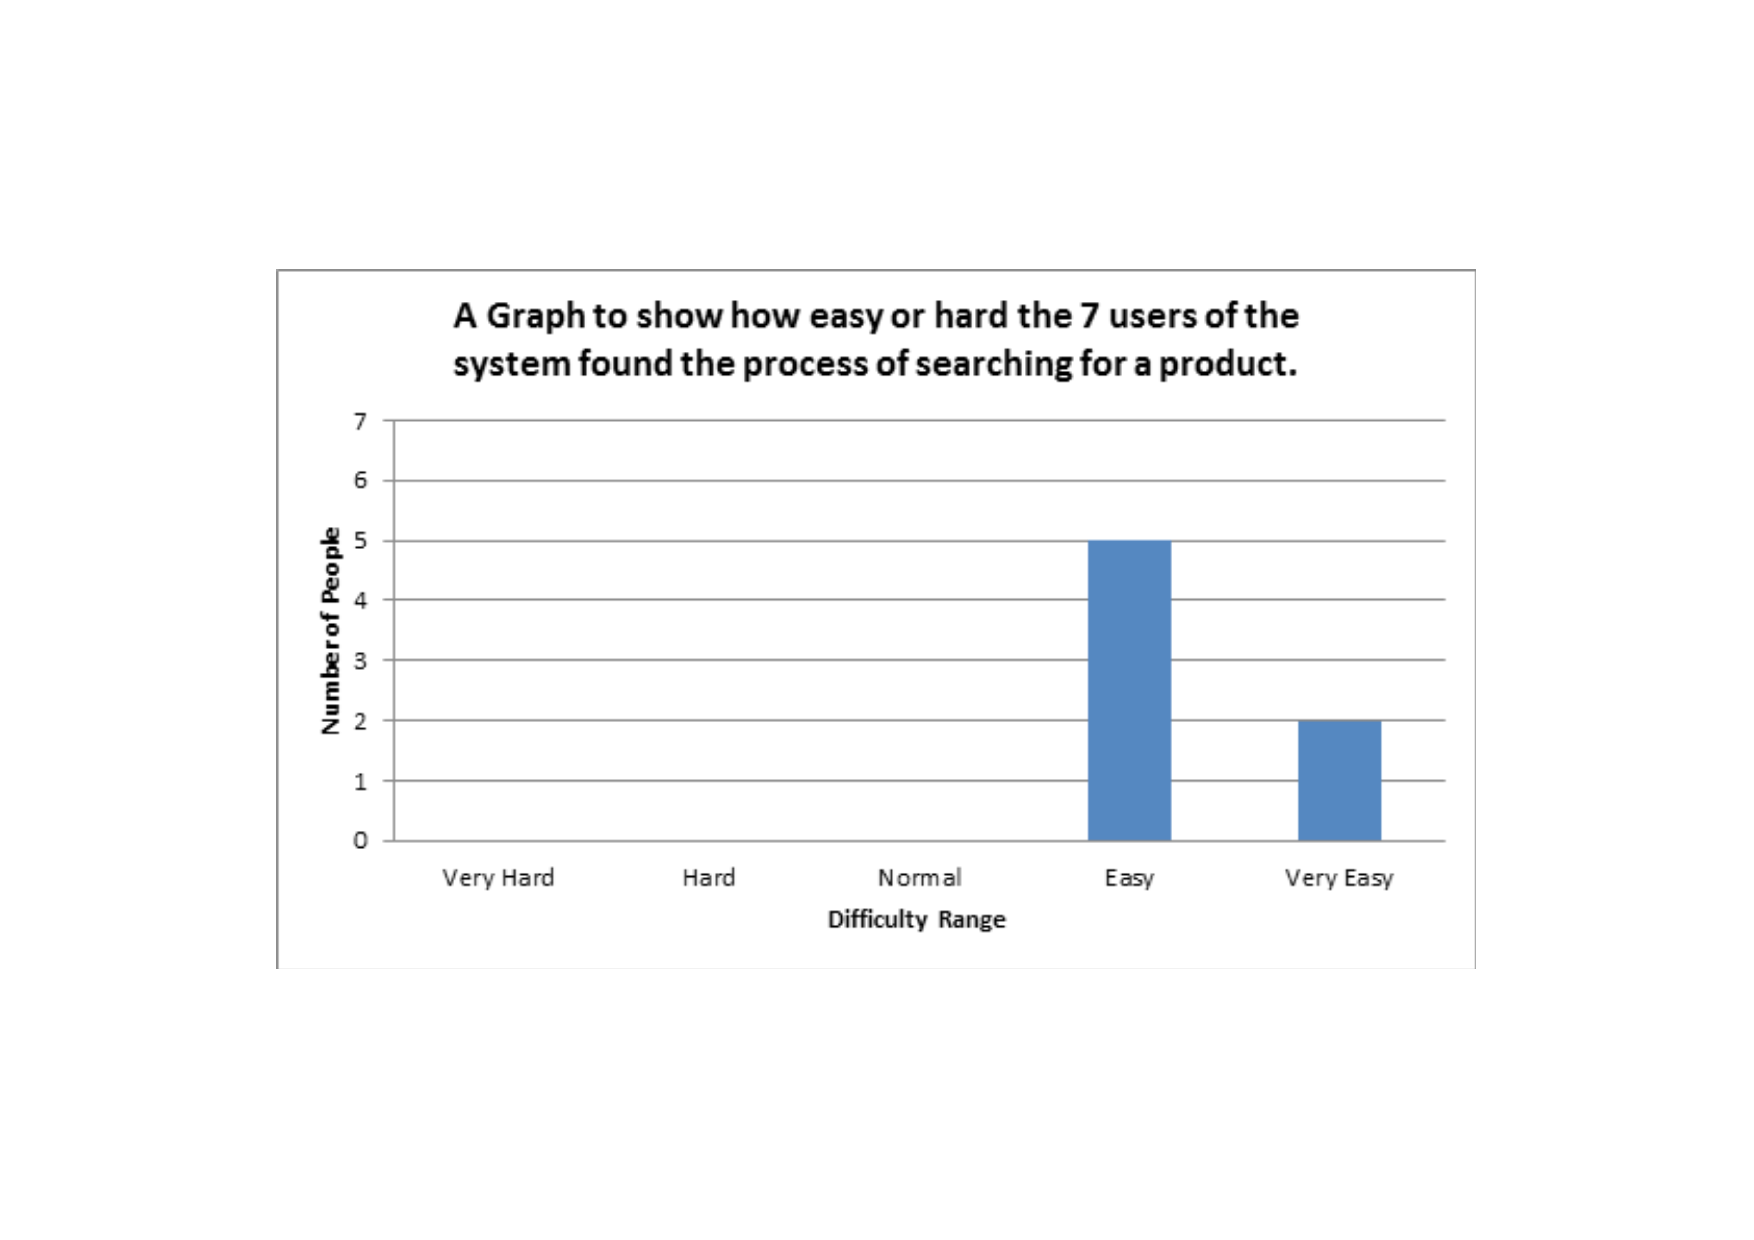
\includegraphics[width = \textwidth]{./Evaluationimages/graph3.pdf}
\end{figure}

The graph shows that all 7 users found the process of searching for a product to be either easy or very easy. This concludes that this objective has been fulfilled, as the objective was that this process should be easy to do, which has been proven by my user feedback.


\pagebreak
\subsubsection{-The system as a whole, should be clear and easy to use.}
\textbf{Was the Objective Fulfilled?} \newline

\textbf{\large{This objective has been fulfilled successfully}}

The system can be navigated easily using the Menu bar, almost all data input fields are clearly labelled so that the user knows what data should be input into the data field.

\textbf{Evidence} \newline

This can be evaluated by taking the general feedback from the ease of use from the different components of the system. Figure \ref{graph1} on page \pageref{page1} concludes that data can be added to the system relatively easily, figure \ref{graph2} on page \pageref{graph2}, shows that data can be edited in the system relatively easily and figure \ref{graph3} on page \pageref{graph3} shows that searching for a product is easy.

I did not ask the users their opinion on the flow of control between interfaces which would have given stronger evidence that this objective has or hasn't been fulfilled. Using the data in which i have, i can conclude that the system, as a whole is easy to use, however, I could have acquired more data in the questionnaire to back up this statement. 

\pagebreak
\subsection{Specific Objective Evaluation}



\subsubsection{-For an image to be displayed when an item is searched for (identifying a product if the Product information is unknown}
\textbf{Was the Objective Fulfilled?} \newline


\textbf{\large{This objective was not fulfilled}}

I did not fulfil this objective as i had problems during the implementation stage when displaying the Product Images in a table. Each time the contents of the Product Table changed, the system would stop responding for about 10-15 seconds before displaying the images and the contents of the search result. Therefore, in order to make the flow of control of the system more fluid, i decided to remove this functionality from the system. \newline

\textbf{Evidence} \newline

\begin{figure}[H]
\caption{Evidence that an image is not displayed in the search window.} \label{fig:evaluation-8}
\hfill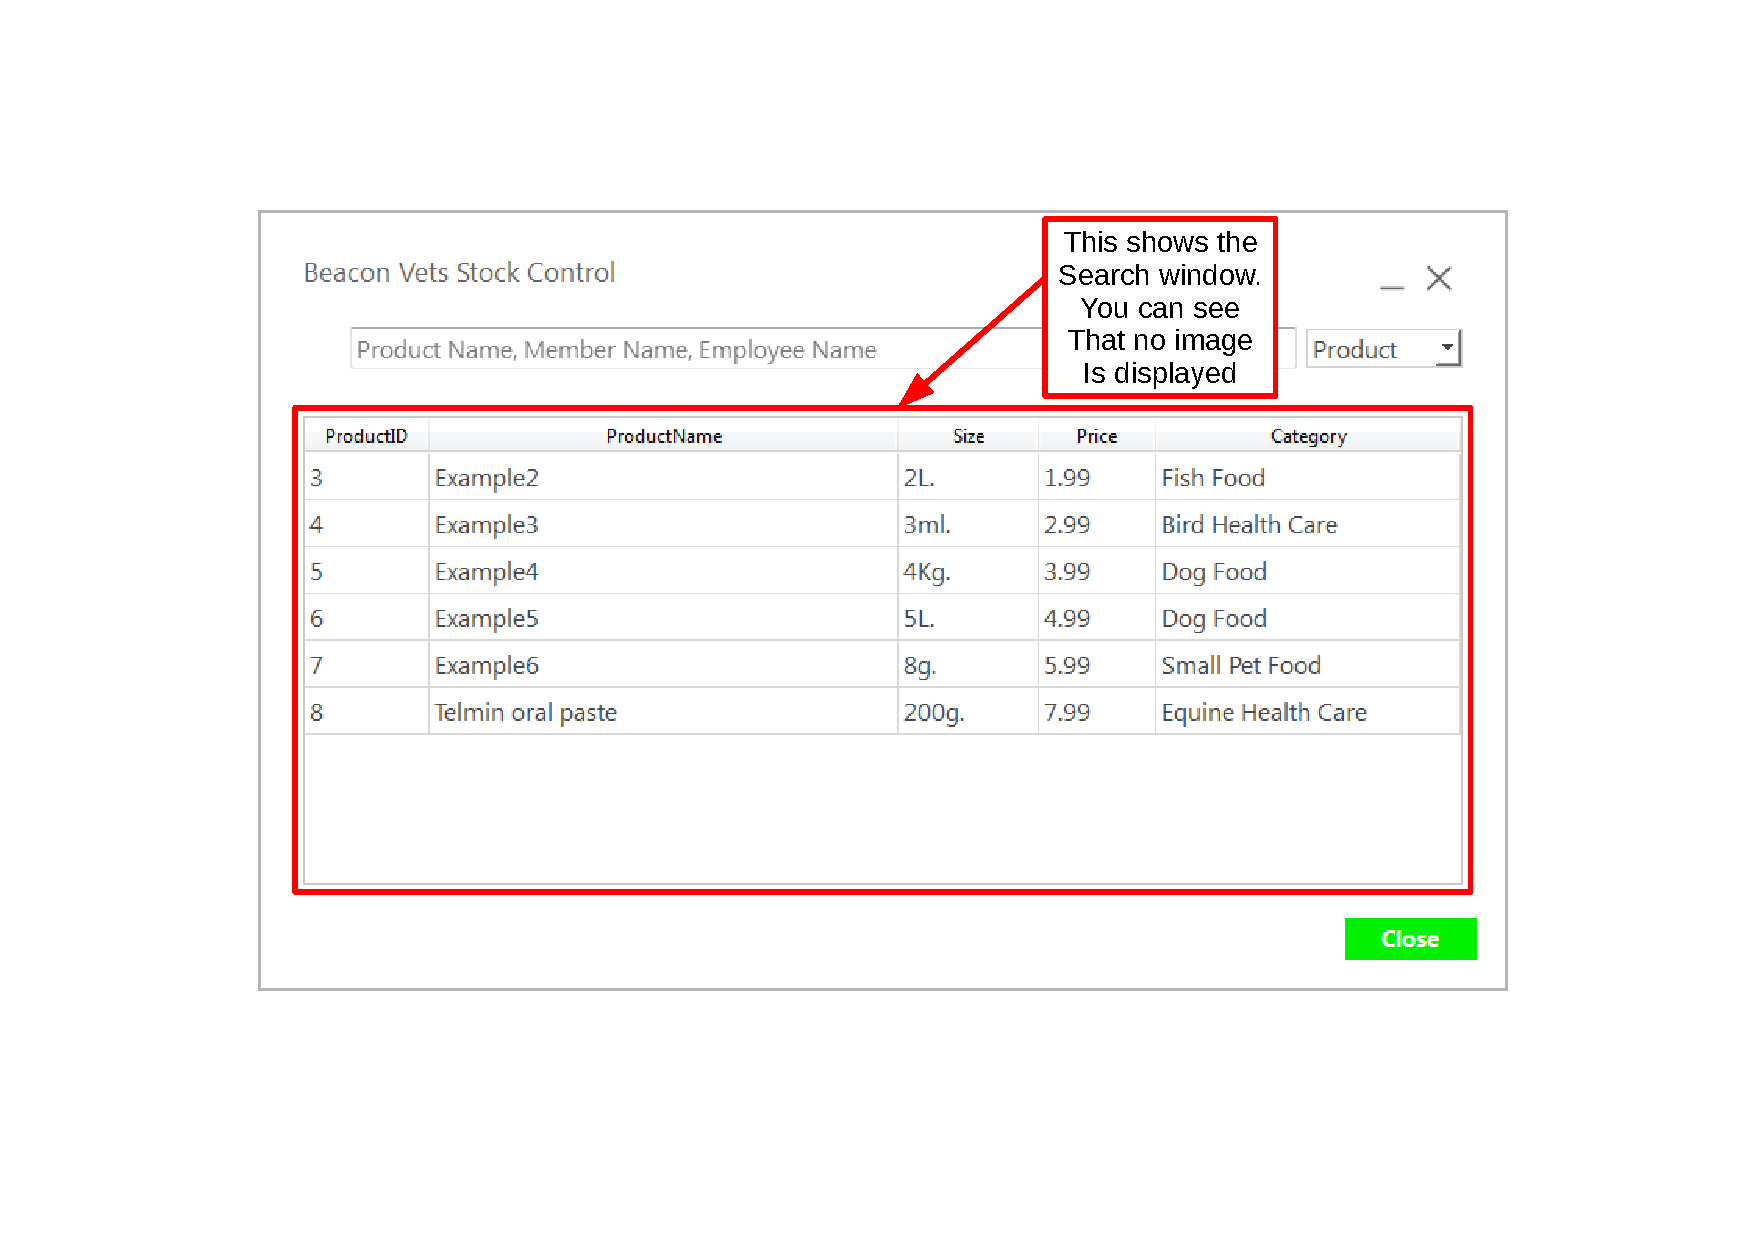
\includegraphics[width = \textwidth]{./Evaluationimages/evaluation-8.pdf}
\end{figure}

I would have created a graph to represent the results from Question 4 in the questionnaire, which asked the users whether or not an image was displayed.However, all 7 users said an image was not displayed in the search window which was as expected. This was the reason why i did not create a graph to display the results.  This concludes this objective has not been fulfilled.



\pagebreak
\subsubsection{For the Stock control system to be integrated with the process of selling items. This is so that the stock is automatically updated when a product is sold.}
\label{For the Stock control system to be integrated with the process of selling items. This is so that the stock is automatically updated when a product is sold.}
\textbf{Was the Objective Fulfilled?} \newline

\textbf{\large{This objective was fulfilled}}

When a customer purchases an item(s), when the invoice is saved to the system, the system automatically deducts the quantity of each product the customer purchased, from the current stock of the product.\newline

\textbf{Evidence} \newline
\label{automatic-stock-evidence}

\begin{figure}[H]
\caption{Evidence that stock is updated automatically in the system.} \label{fig:evaluation-9-1}
\hfill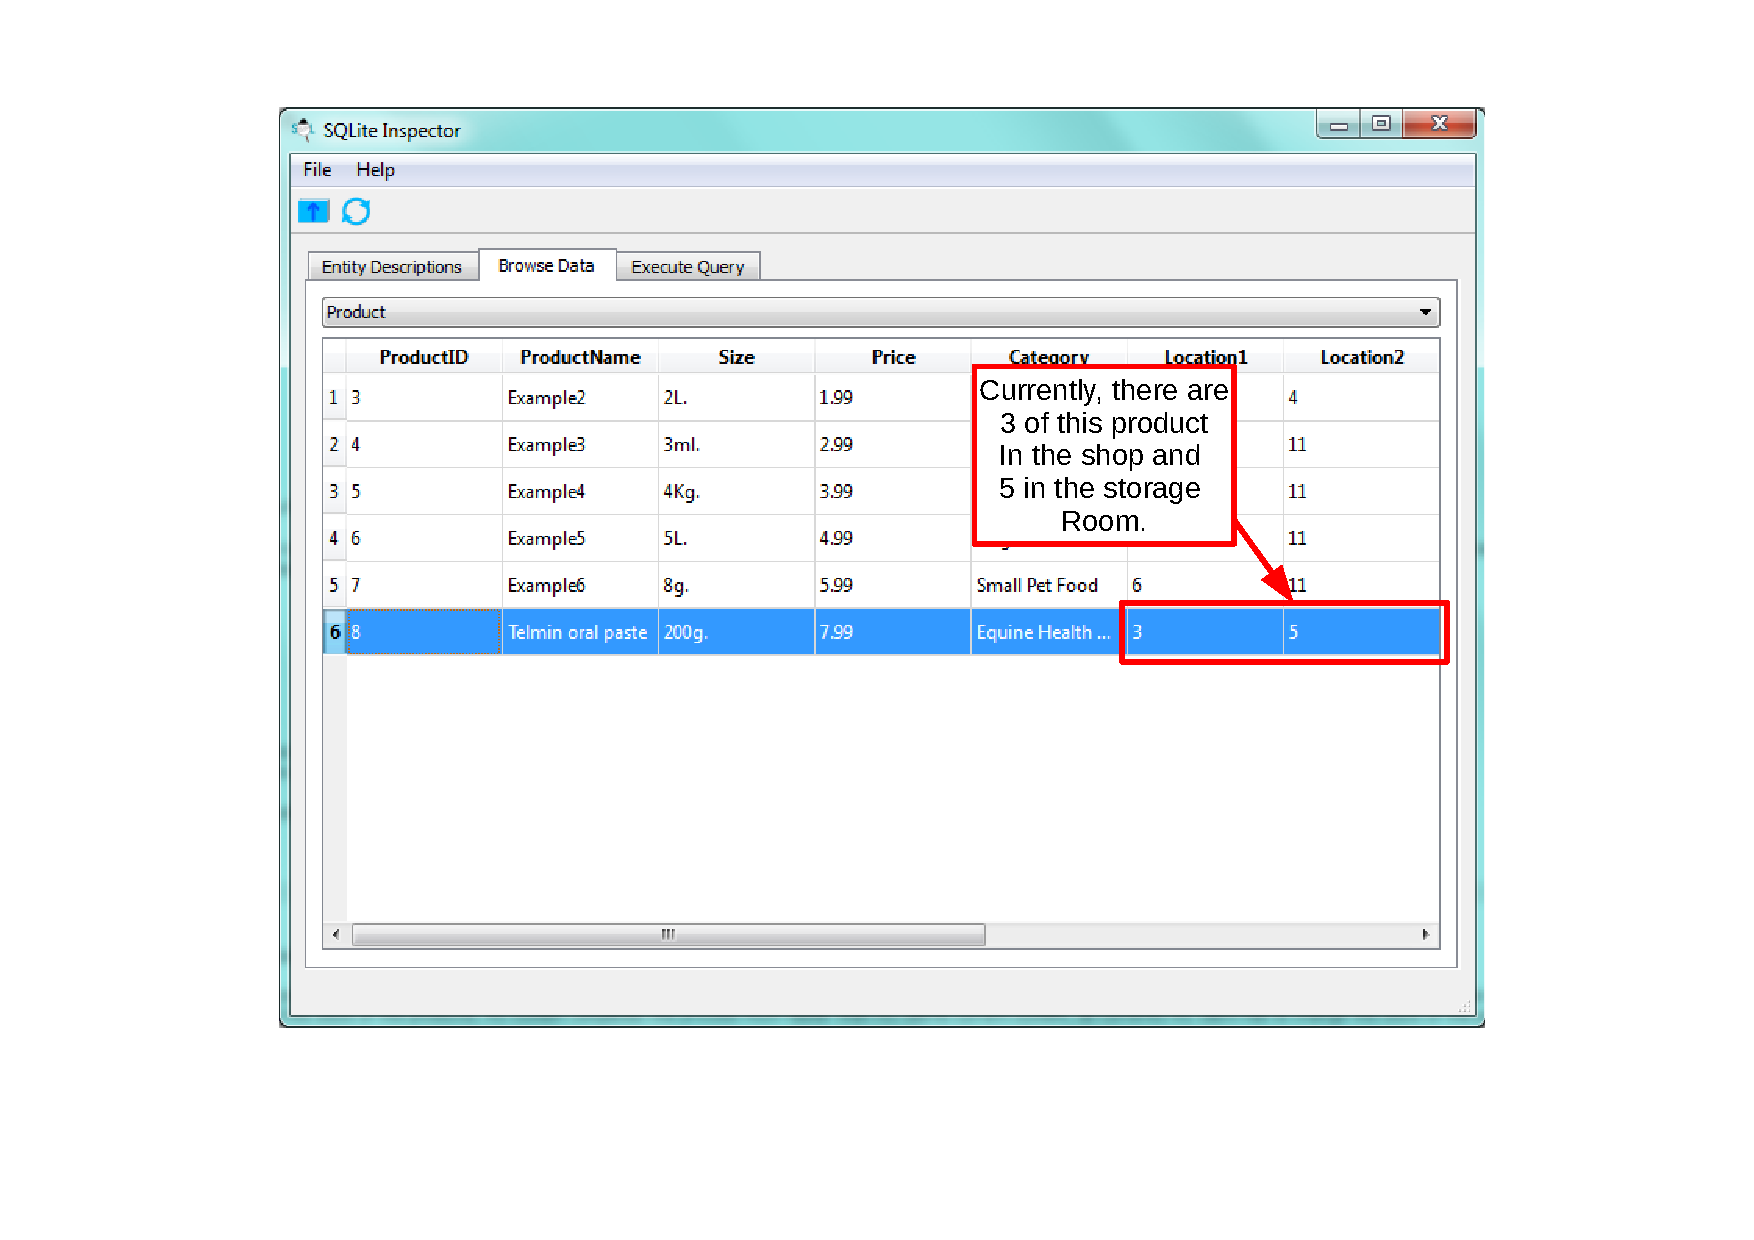
\includegraphics[width = \textwidth]{./Evaluationimages/evaluation-9-1.pdf}
\end{figure}

\begin{figure}[H]
\caption{Evidence that stock is updated automatically in the system.} \label{fig:evaluation-9-2}
\hfill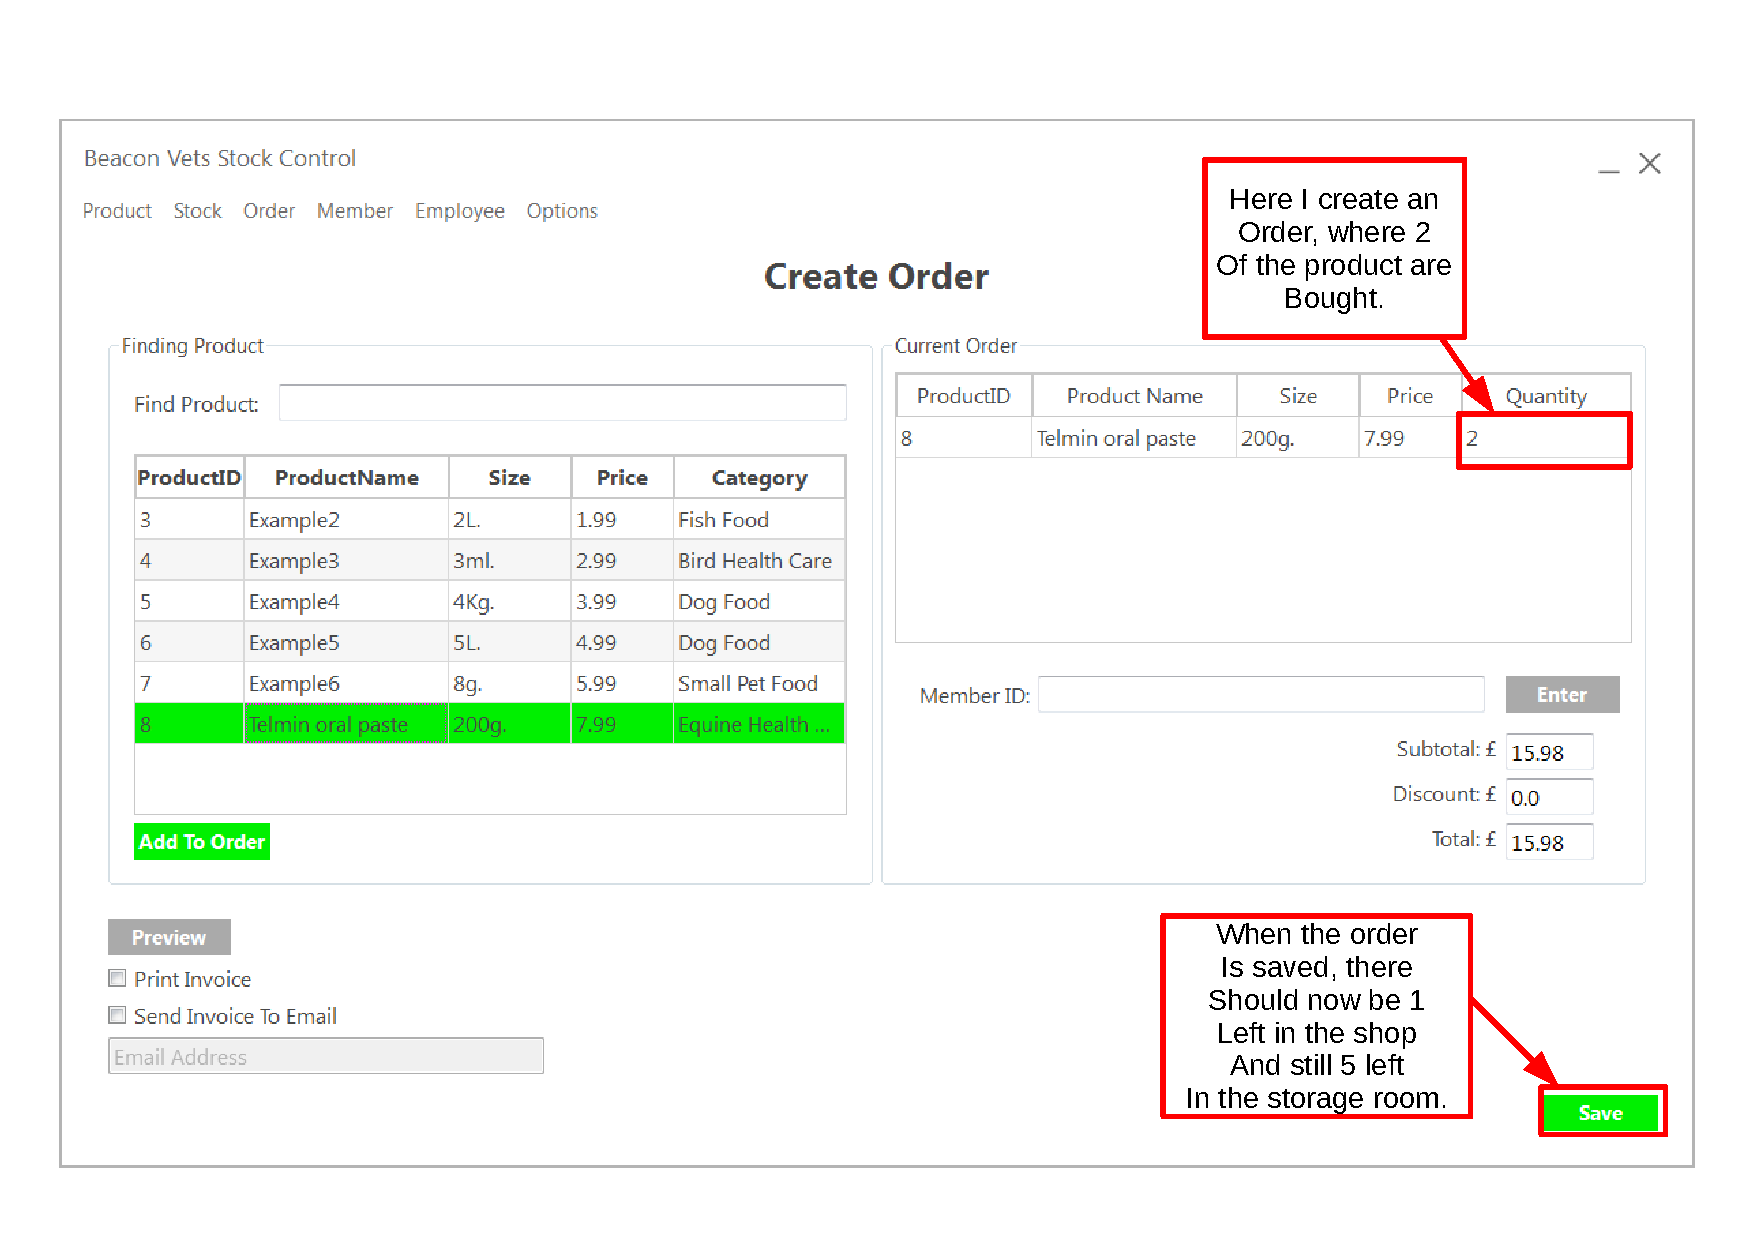
\includegraphics[width = \textwidth]{./Evaluationimages/evaluation-9-2.pdf}
\end{figure}

\begin{figure}[H]
\caption{Evidence that stock is updated automatically in the system.} \label{fig:evaluation-9-3}
\hfill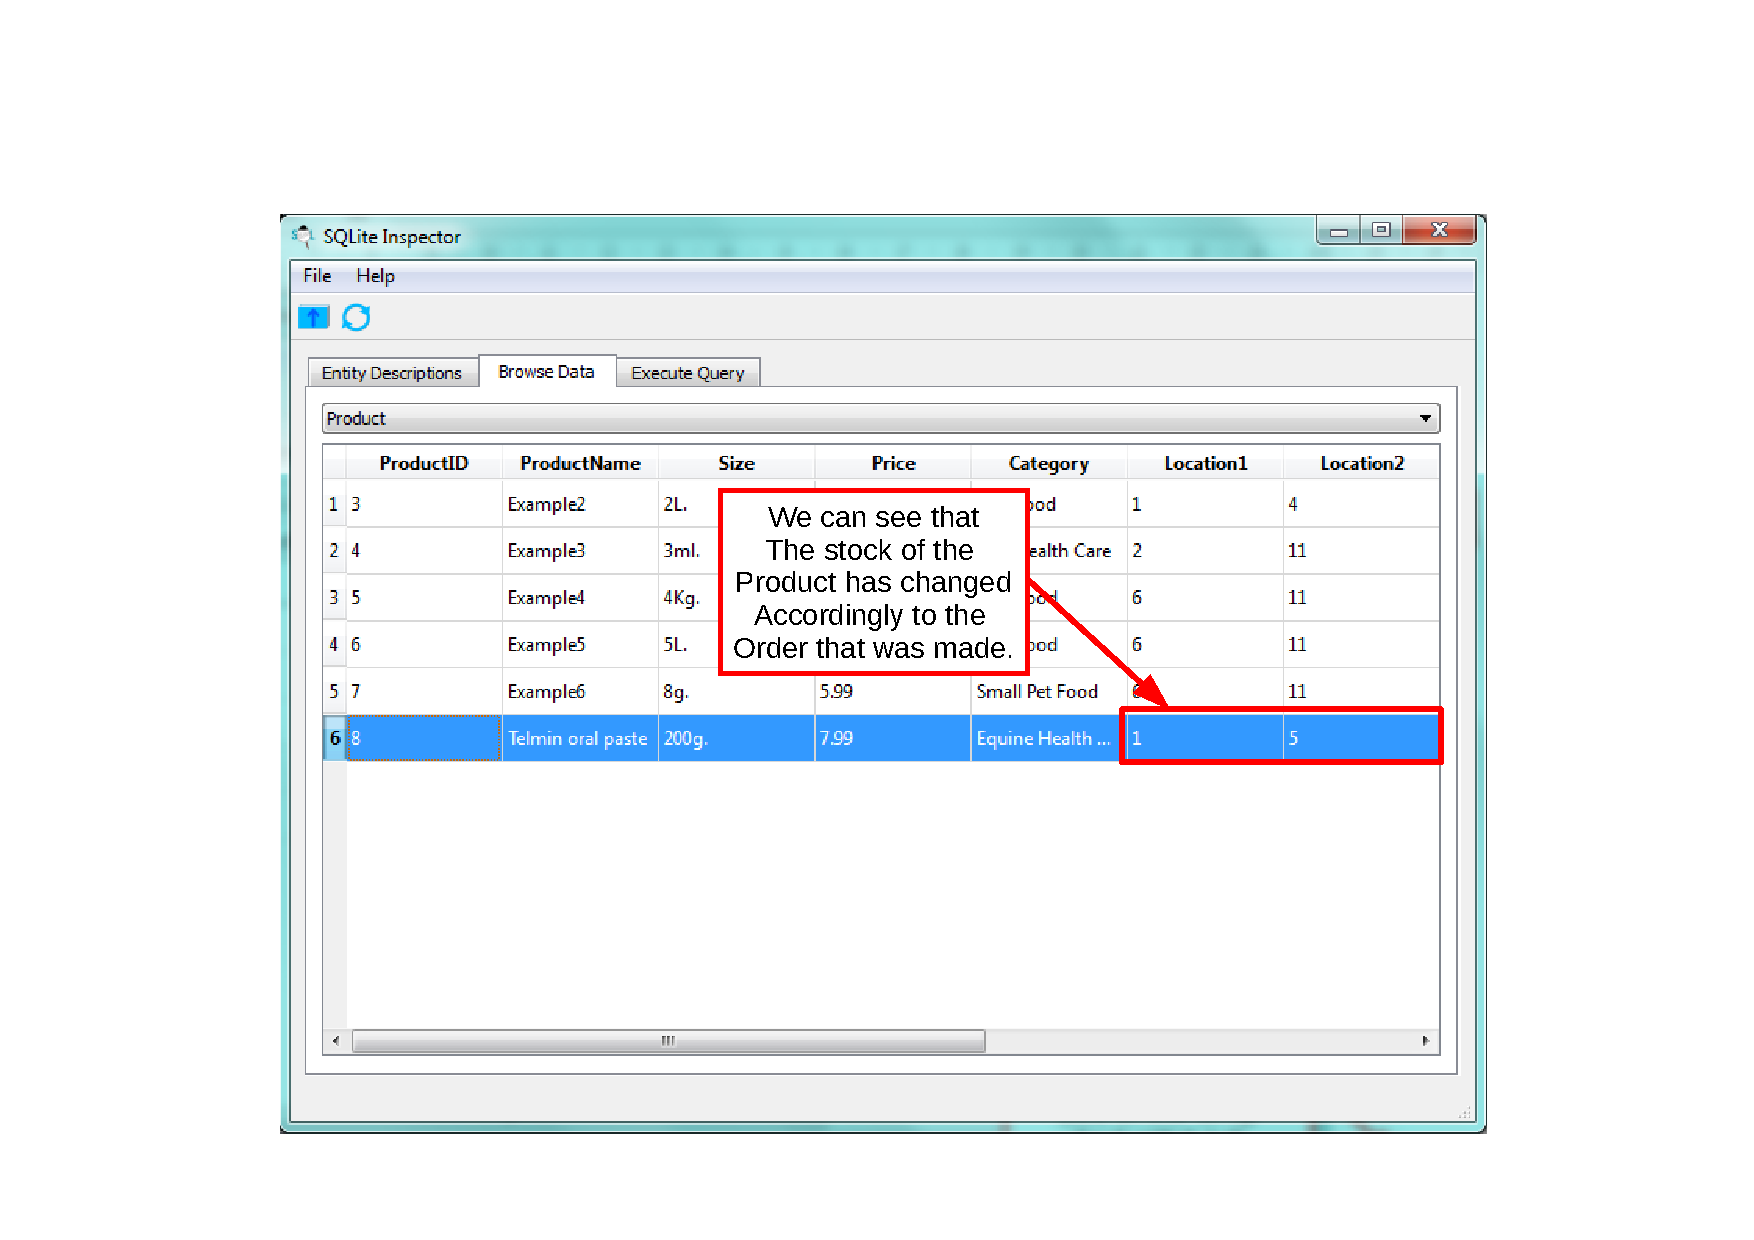
\includegraphics[width = \textwidth]{./Evaluationimages/evaluation-9-3.pdf}
\end{figure}

This objective was fulfilled during the Implementation and Testing stage whilst developing the system. During the implementation stage i ensured that the algorithm used to change the stock worked successfully and implemented the algorithm into my system. The user feedback on this area from the questionnaire was to ensure that it was working correctly and to find any problems, if any, with this area of the system. No problems were highlighted by the 7 users from my questionnaire, which strongly suggests this area functions correctly. Therefore, I have concluded that this objective has been fulfilled.



\pagebreak
\subsubsection{-For the new process of selling products to be quicker, to minimize the time for people queuing.}
\textbf{Was the Objective Fulfilled?} \newline

\textbf{\large{This objective was not fulfilled}}

This objective was not fulfilled because currently, my client uses a bar code scanner that automatically finds the product in the system and adds it to the order when the bar code is scanned. This objective has been poorly worded, as my system could not be any faster than the current system of selling products without using this method of adding products to an order. However, if you combine the time spent creating the order and time spent changing all the stock of the products, my system completes this process much faster than my clients current system, as currently my client has to change the stock of the products each day to match the sales made that day. This process is done automatically in my system which is evidenced in figure \ref{fig:evaluation-9-1}, \ref{fig:evaluation-9-2}, \ref{fig:evaluation-9-3}, on  page \pageref{automatic-stock-evidence}. \newline

\textbf{Evidence} \newline

Please refer to figure \ref{fig:evaluation-9-1}, \ref{fig:evaluation-9-2}, \ref{fig:evaluation-9-3}, on  page \pageref{automatic-stock-evidence} for evidence that the stock automatically changes when an order is made.

It was also raised that an additional feature should be to integrate the system to use with the bar code scanner. This point was raised in questionnaires 1 and 5 in question 15. This would greatly increase the speed of selling products. None of the users raised any issues in the questionnaire when creating an order in question 6 of the questionnaire, which concludes there are most likely no problems with this area of the system, which could cause creating orders longer than expected.




\pagebreak
\subsubsection{-For the current stock to automatically update when the products are bought}
\textbf{Was the Objective Fulfilled?} \newline

\textbf{\large{This objective has previously been fulfilled}}

This objective has already been fulfilled in the "-For the Stock control system to be integrated with the process of selling items''. This is so that the stock is automatically updated when a product is sold" objective.

\textbf{Evidence} \newline

Please refer to figure \ref{fig:evaluation-9-1}, \ref{fig:evaluation-9-2}, \ref{fig:evaluation-9-3}, on  page \pageref{automatic-stock-evidence} for evidence that the stock automatically changes when an order is made.



\pagebreak
\subsubsection{-For a reminder message to pop up when stock needs to be moved from storage to the front of the vets. }
\textbf{Was the Objective Fulfilled?} \newline

\textbf{\large{This objective has been fulfilled}}

When a user logs into the system, the system will check if any products need to be moved between locations or if any products need to be restocked. If there are less than 5 of a specific product in the Shop then the user will be told that stock needs to be moved form the storage room to the shop and if the total stock of the product is less than 5 then the user will be told that that product needs to be restocked.\newline

\textbf{Evidence} \newline

\begin{figure}[H]
\caption{Evidence that the employee is reminded when stock needs to be moved between locations.} \label{fig:evaluation-10-1}
\hfill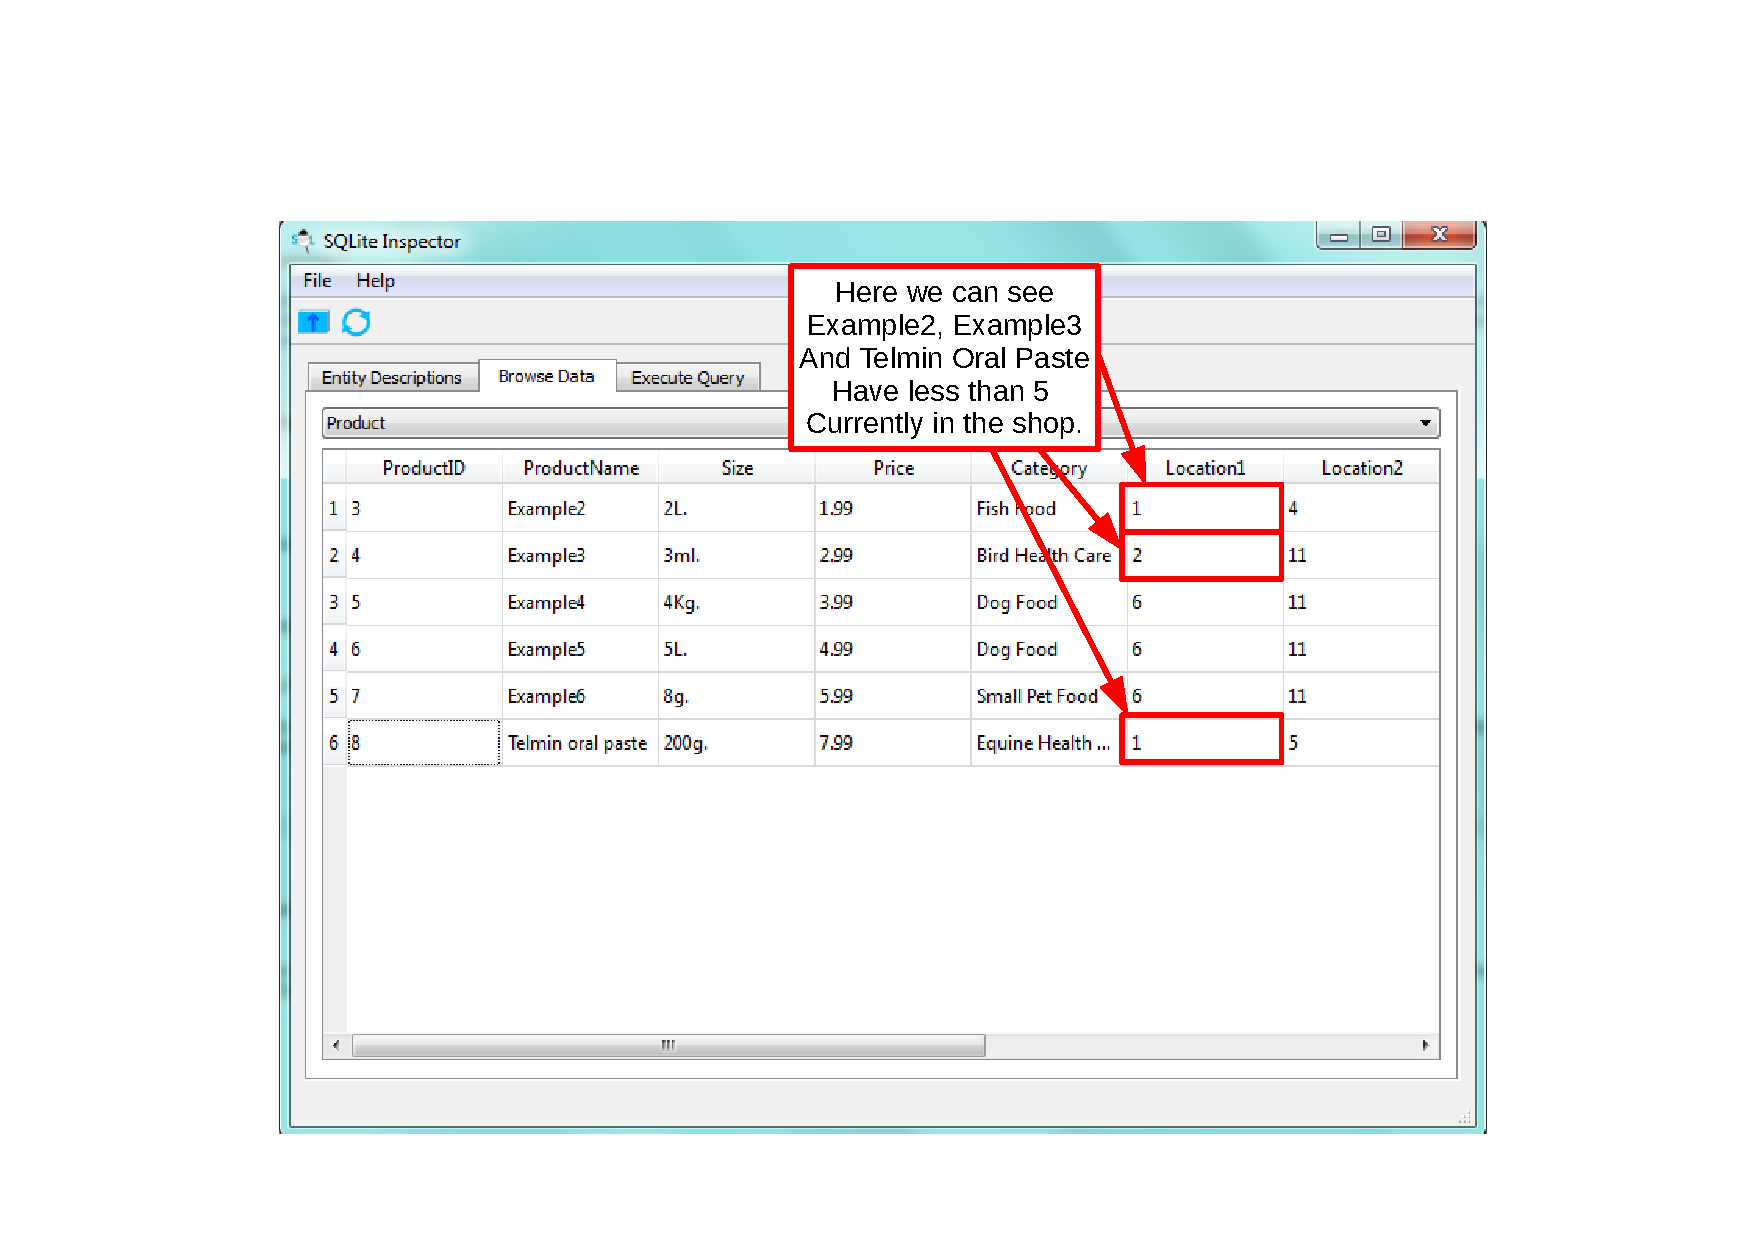
\includegraphics[width = \textwidth]{./Evaluationimages/evaluation-10-1.pdf}
\end{figure}

\begin{figure}[H]
\caption{Evidence that the employee is reminded when stock needs to be moved between locations.} \label{fig:evaluation-10-2}
\hfill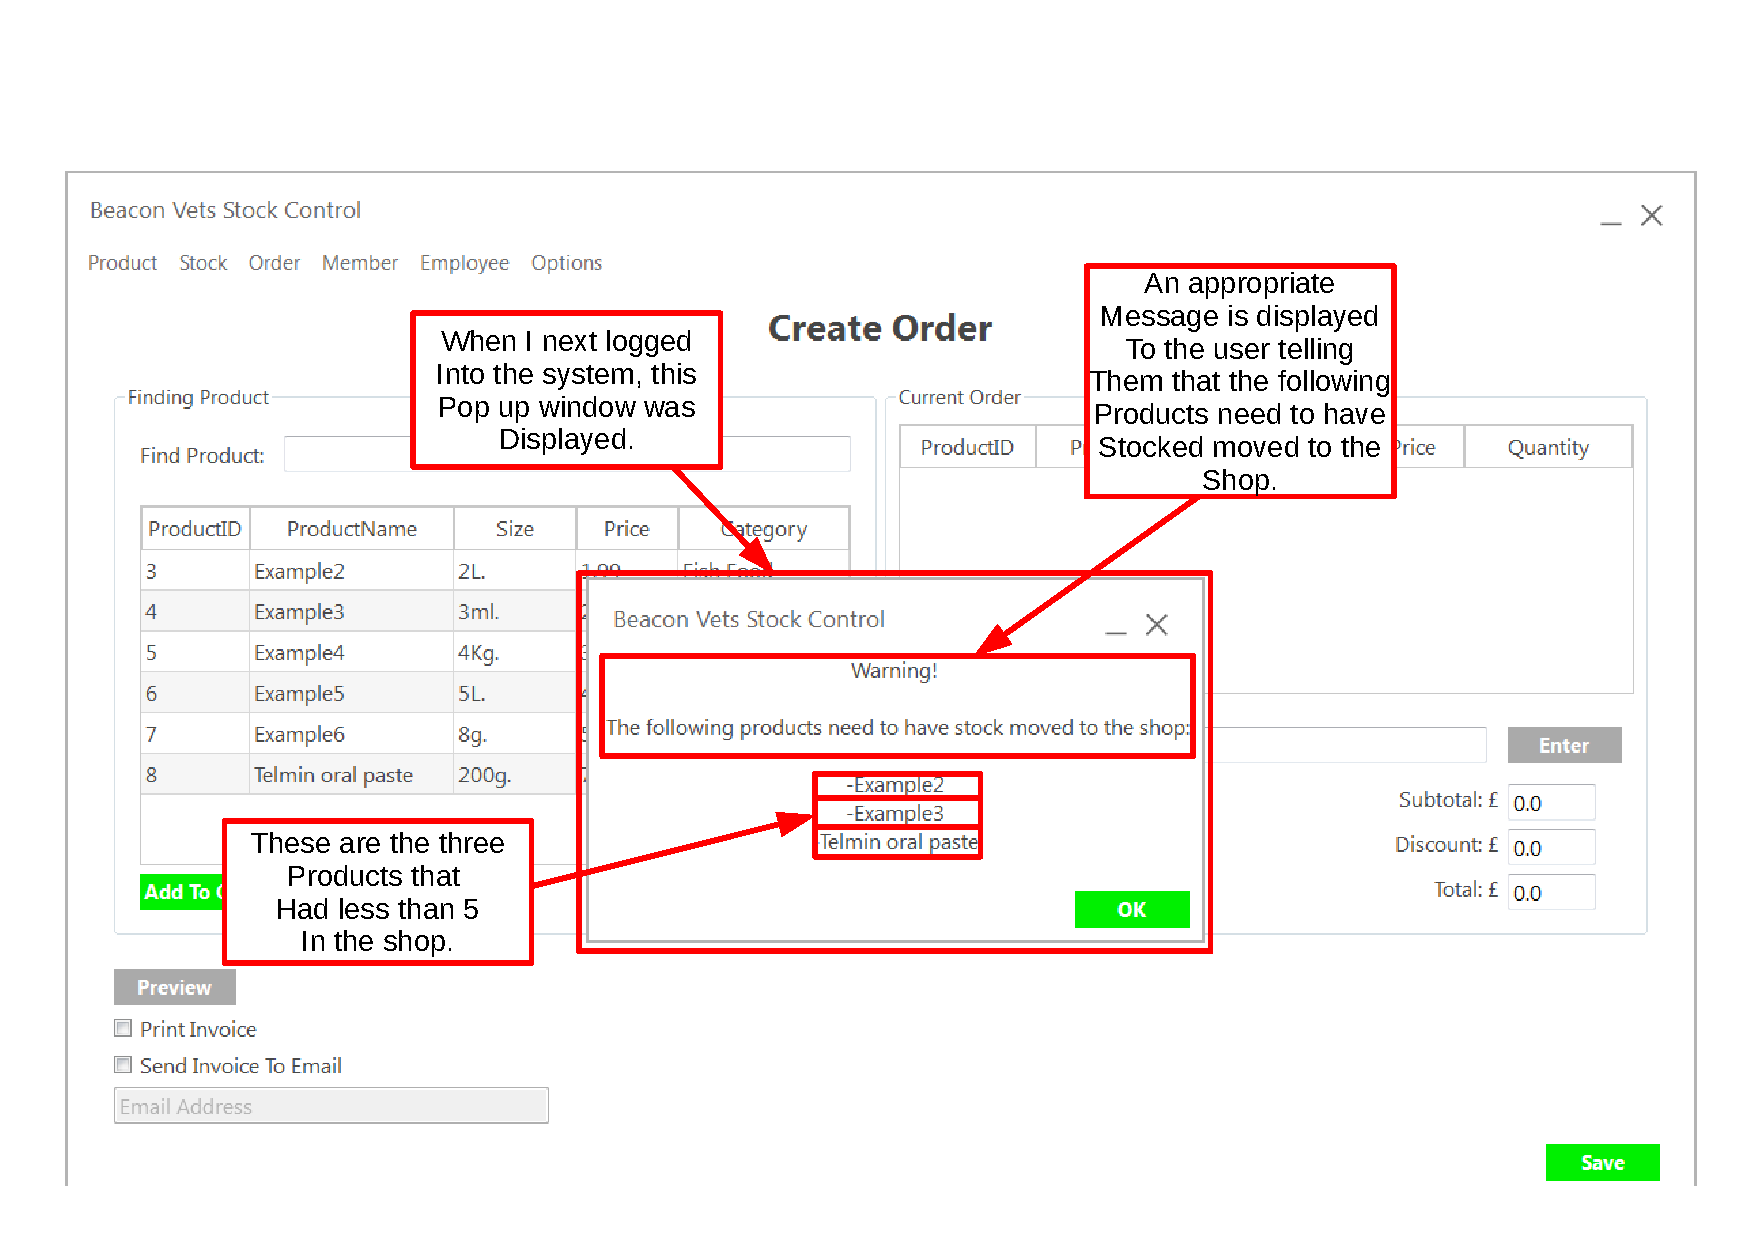
\includegraphics[width = \textwidth]{./Evaluationimages/evaluation-10-2.pdf}
\end{figure}

\begin{figure}[H]
\caption{Evidence that the employee is reminded when the total stock needs to be updated.} \label{fig:evaluation-10-3}
\hfill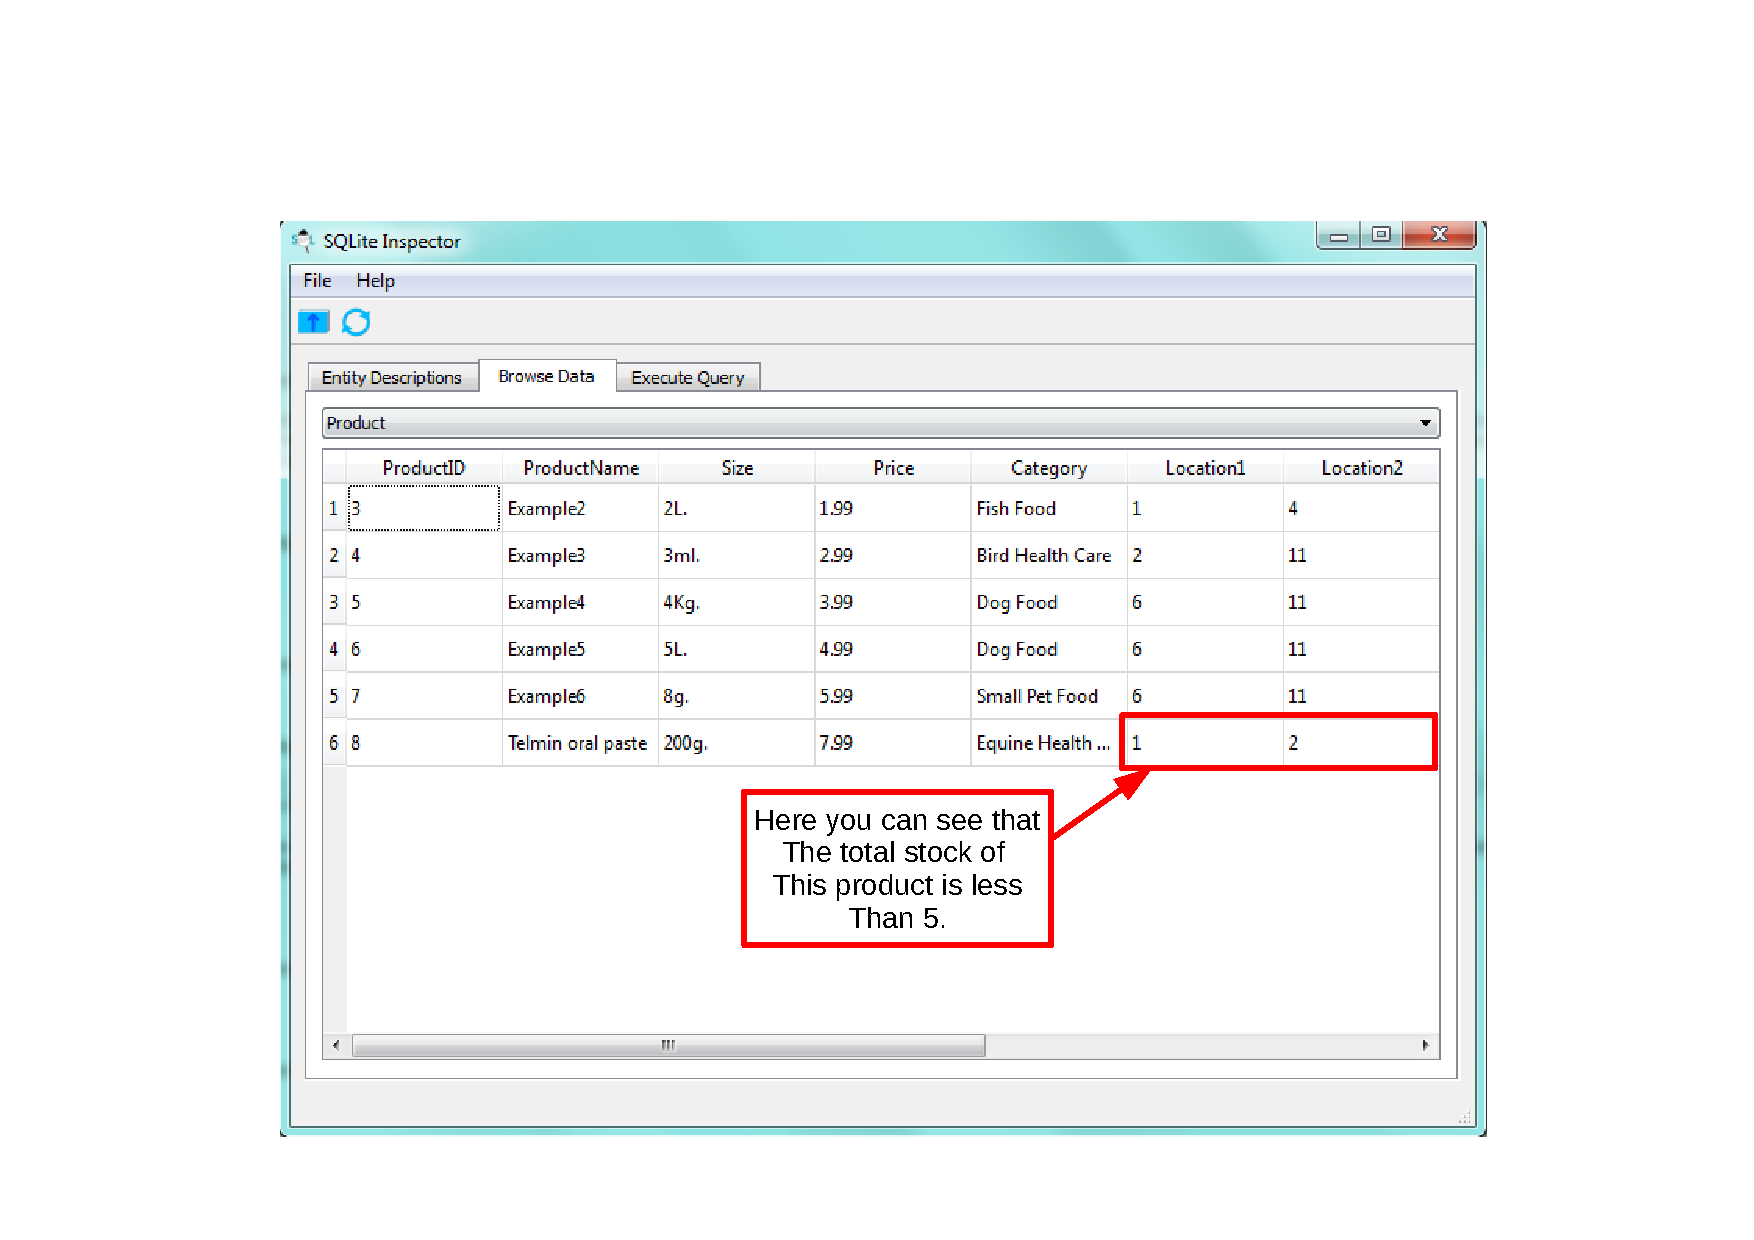
\includegraphics[width = \textwidth]{./Evaluationimages/evaluation-10-3.pdf}
\end{figure}

\begin{figure}[H]
\caption{Evidence that the employee is reminded when the total stock needs to be updated.} \label{fig:evaluation-10-4}
\hfill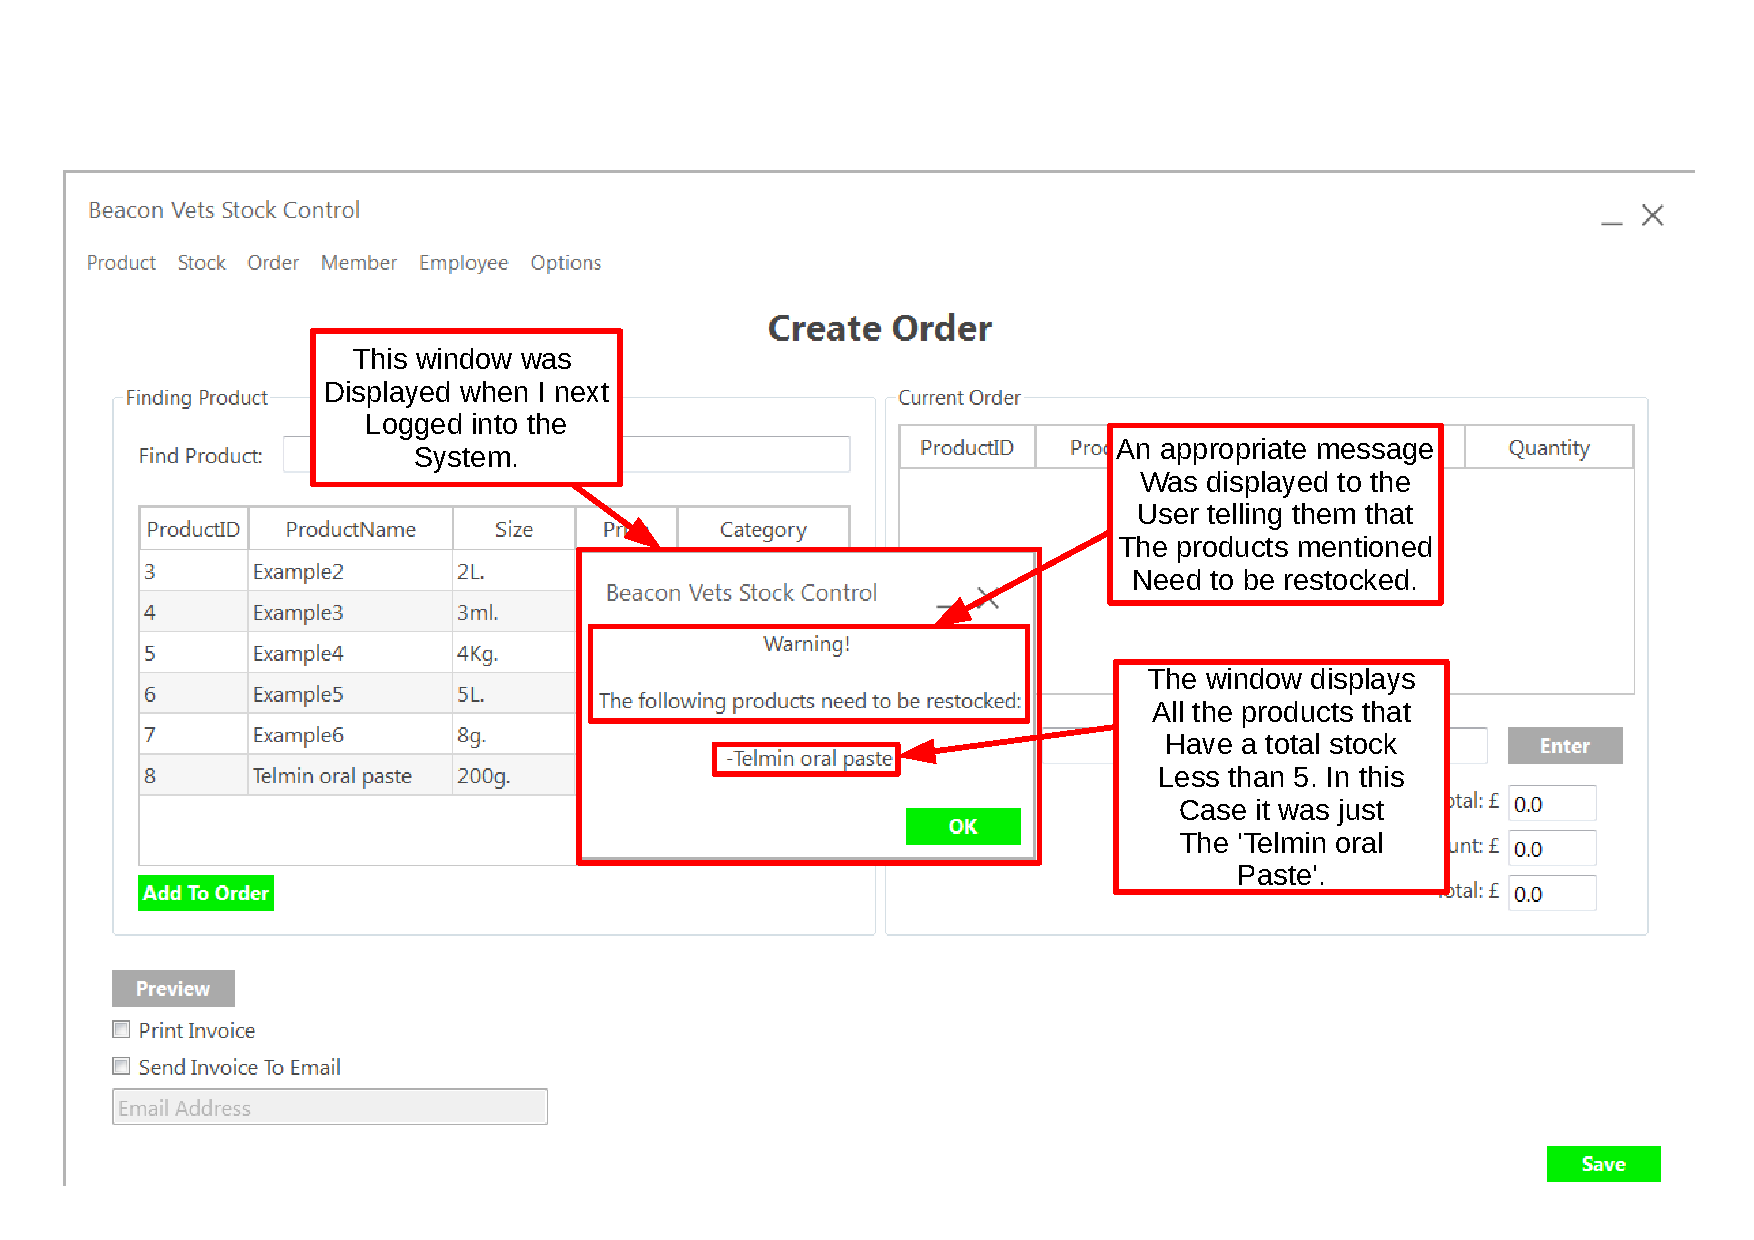
\includegraphics[width = \textwidth]{./Evaluationimages/evaluation-10-4.pdf}
\end{figure}

This feature was evaluated during the implementation and testing phase to ensure that it worked correctly. If there were any problems with this area, in which users may have come across that i did not, they could have highlighted it in Question 7 of the questionnaire. No problems were found during the implementation and no problems we raised by the users in the questionnaire, concluding that this area functions correctly, meaning this objective has been fulfilled.


\pagebreak
\subsubsection{-For each and every product to be categorised for easy identification is the Product Name and ID is unknown.}
\textbf{Was the Objective Fulfilled?} \newline

\textbf{\large{This objective has been fulfilled}}

This objective has been fulfilled when the user adds a product to the system they must choose from two drop down menus (QComboBox) in order to categorise the product. First they choose the animal the product is targeted at, i.e horse, dog, cat and whether the product comes under food or health care. When the user wants to search for all products under, for example, Dog Health Care, they can simply go to the search window and enter 'Dog Health Care' into the search field and the system will return all the products under that category.

\textbf{Evidence} \newline
\label{category-evidence}

\begin{figure}[H]
\caption{Evidence that the the products can be usefully categorised.} \label{fig:evaluation-11-1}
\hfill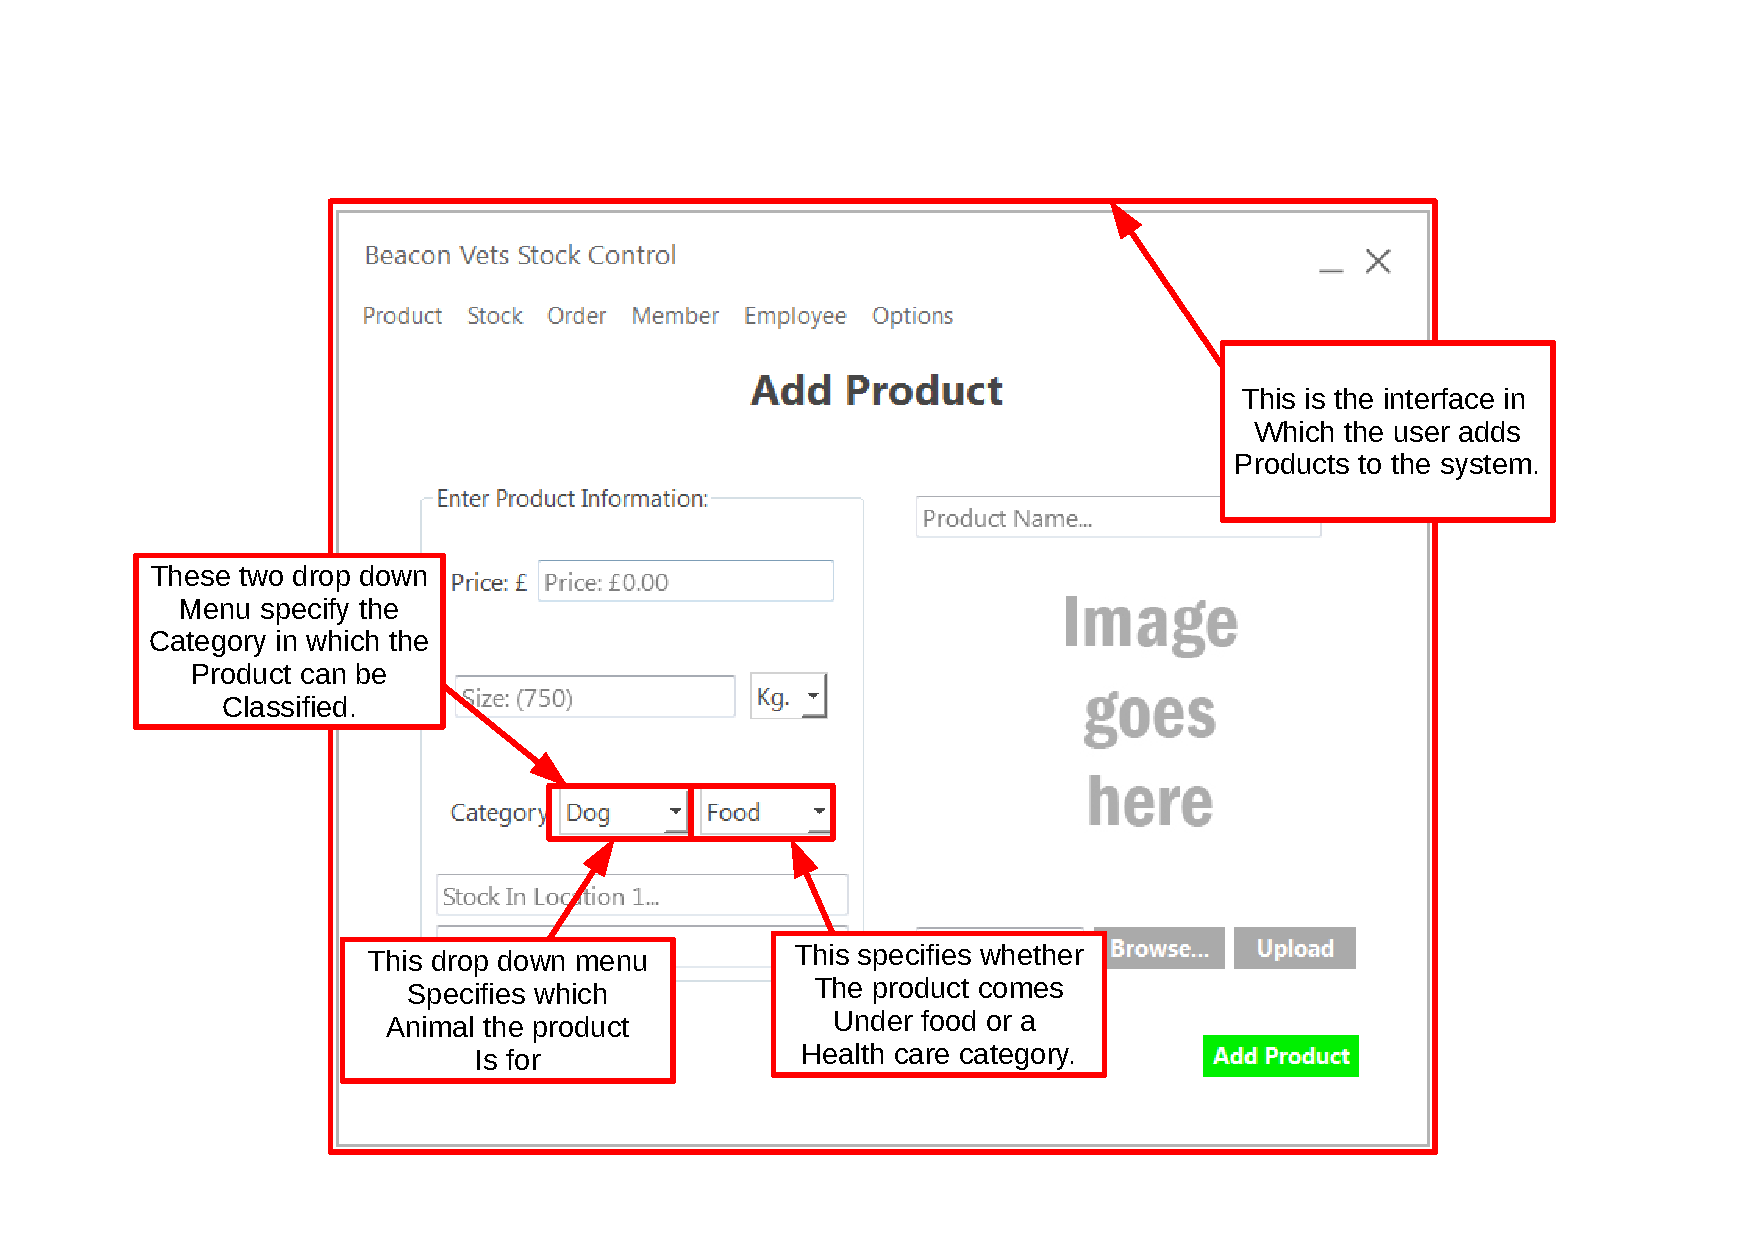
\includegraphics[width = \textwidth]{./Evaluationimages/evaluation-11-1.pdf}
\end{figure}

\begin{figure}[H]
\caption{Evidence that the the products can be usefully categorised.} \label{fig:evaluation-11-2}
\hfill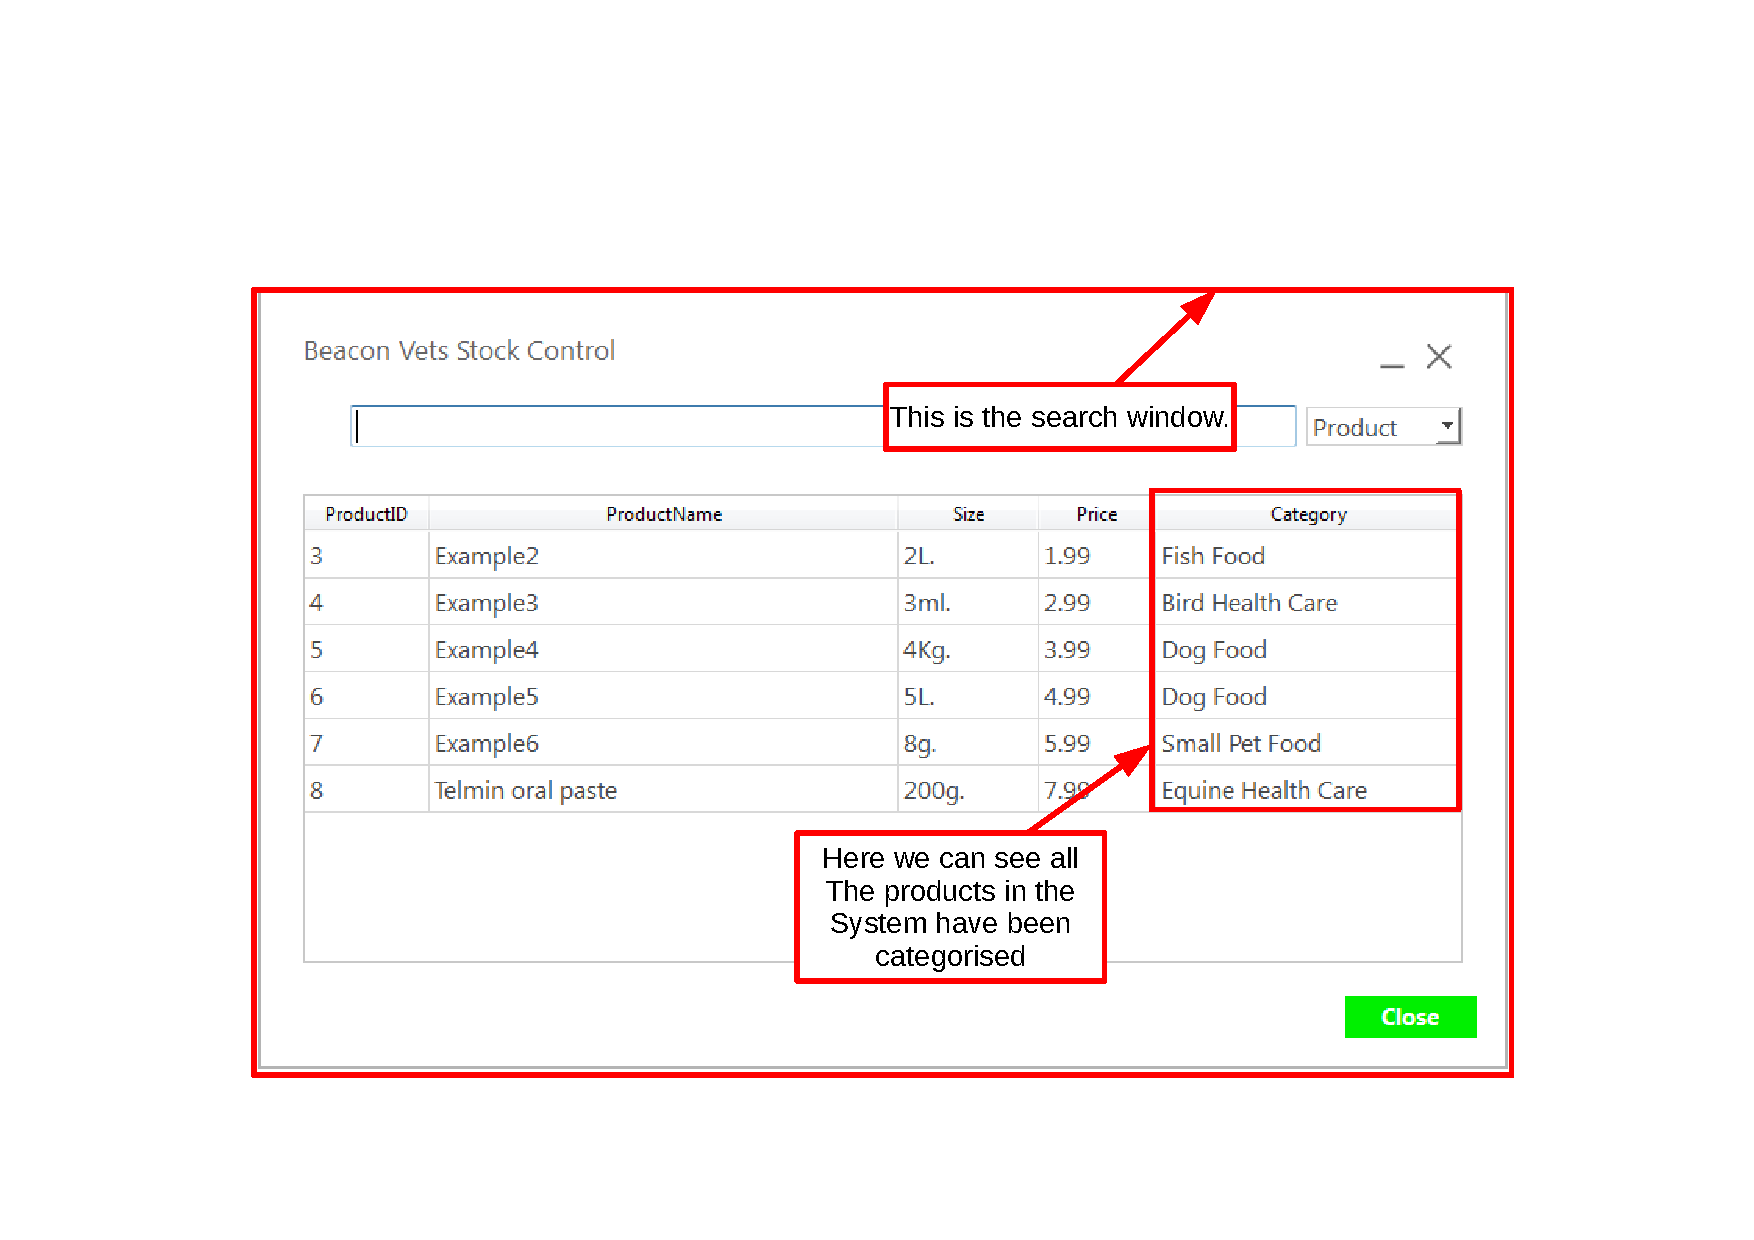
\includegraphics[width = \textwidth]{./Evaluationimages/evaluation-11-2.pdf}
\end{figure}

\begin{figure}[H]
\caption{Evidence that the the products can be usefully categorised.} \label{fig:evaluation-11-3}
\hfill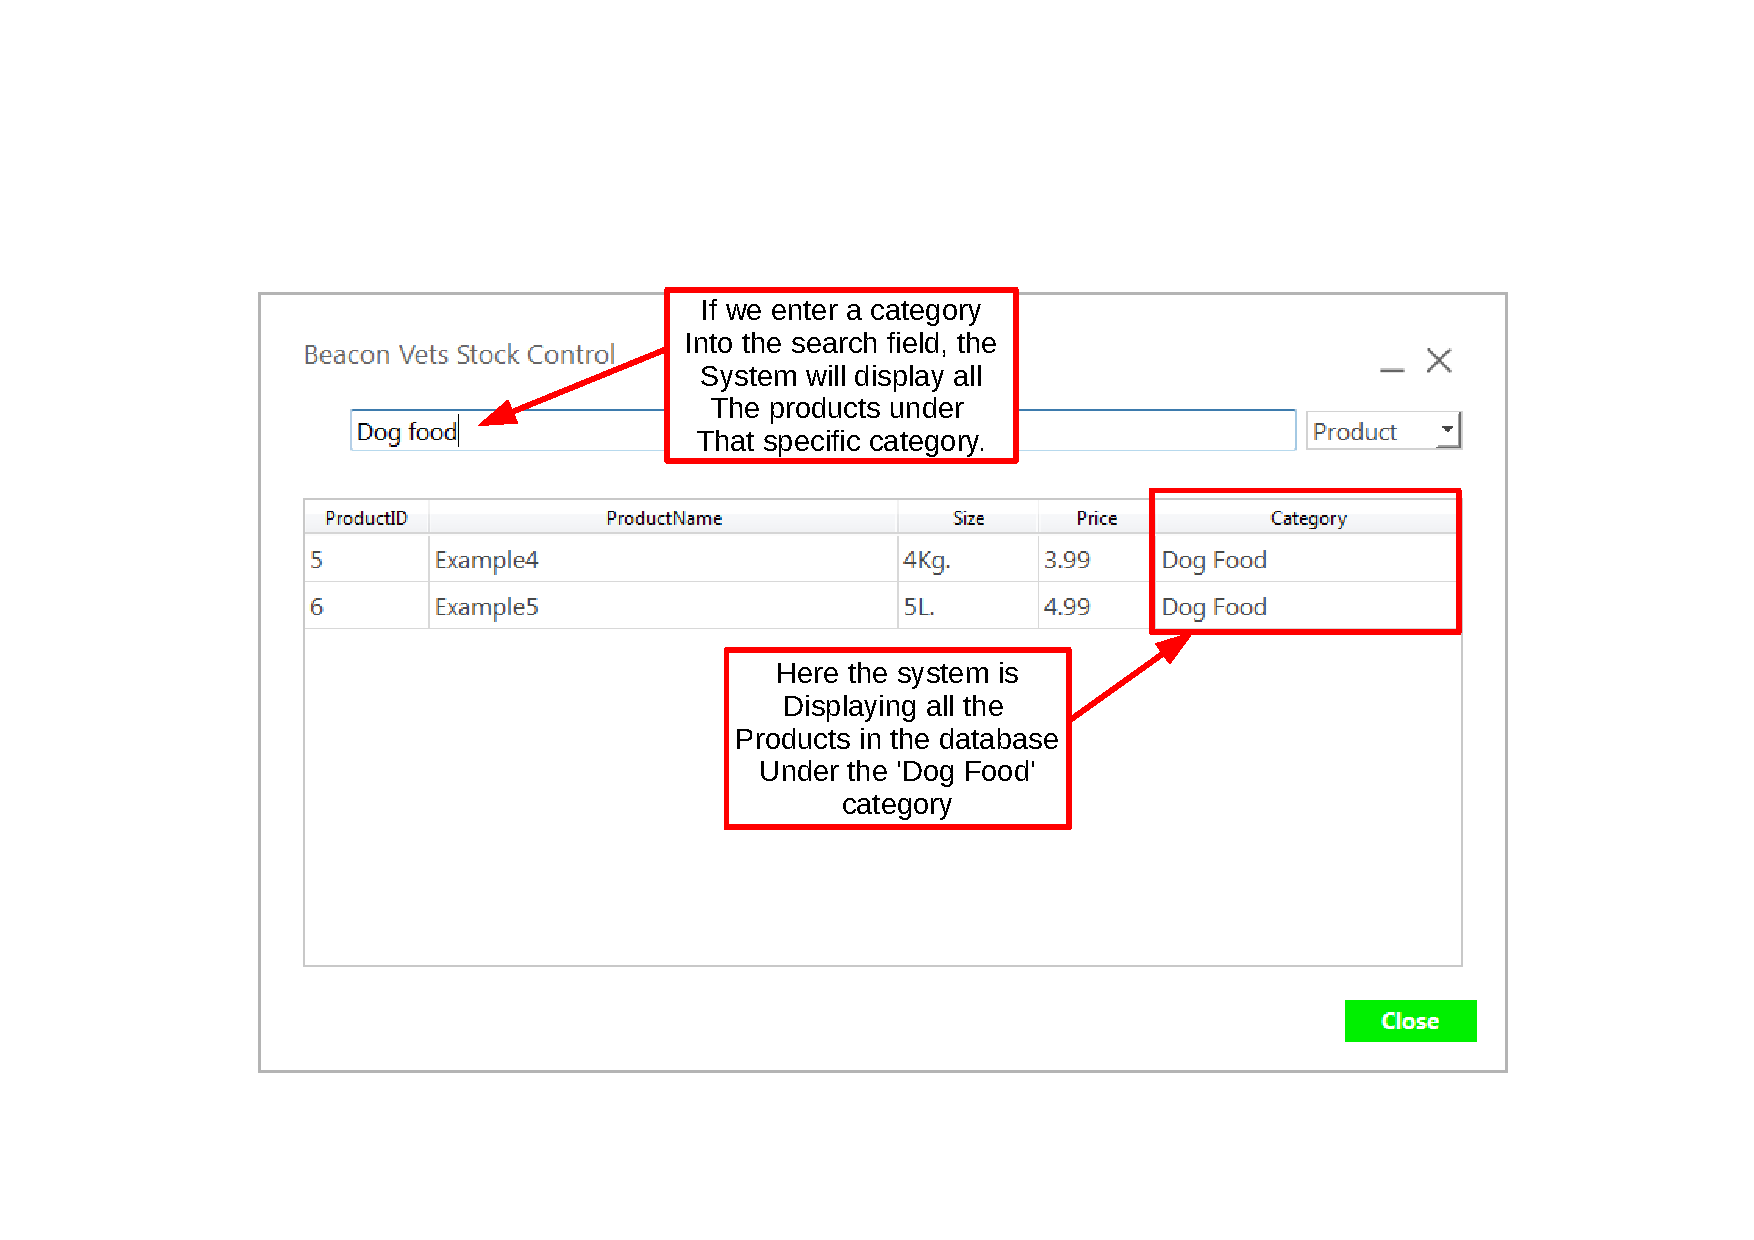
\includegraphics[width = \textwidth]{./Evaluationimages/evaluation-11-3.pdf}
\end{figure}

Again, this objective was evaluated during the Implementation and Testing stage. I ensured that the algorithm used to search for products functioned correctly and included a question (Question 8) in the questionnaire, in which the users could highlight any problems they came across when categorising products. None of the 7 users highlighted any problems with the categorisation process and no problems occured when testing the functionality which concludes that this area functions correctly, which fulfills this objective.




\pagebreak
\subsubsection{-To calculate how much stock will be required for next month.}
\label{stock-eval}
\textbf{Was the Objective Fulfilled?} \newline

\textbf{\large{This objective has been fulfilled}}


The system records the daily and weekly sales of each product. These sales are then plotted to a graph on the stock management interface, which is used to predict the sales for the up coming week. Predicting the sales from the daily sales usually produces are more accurate prediction.

\textbf{Evidence} \newline

\begin{figure}[H]
\caption{Graph displaying weekly sales of a product} \label{fig:graph-evidence-1.pdf}
\hfill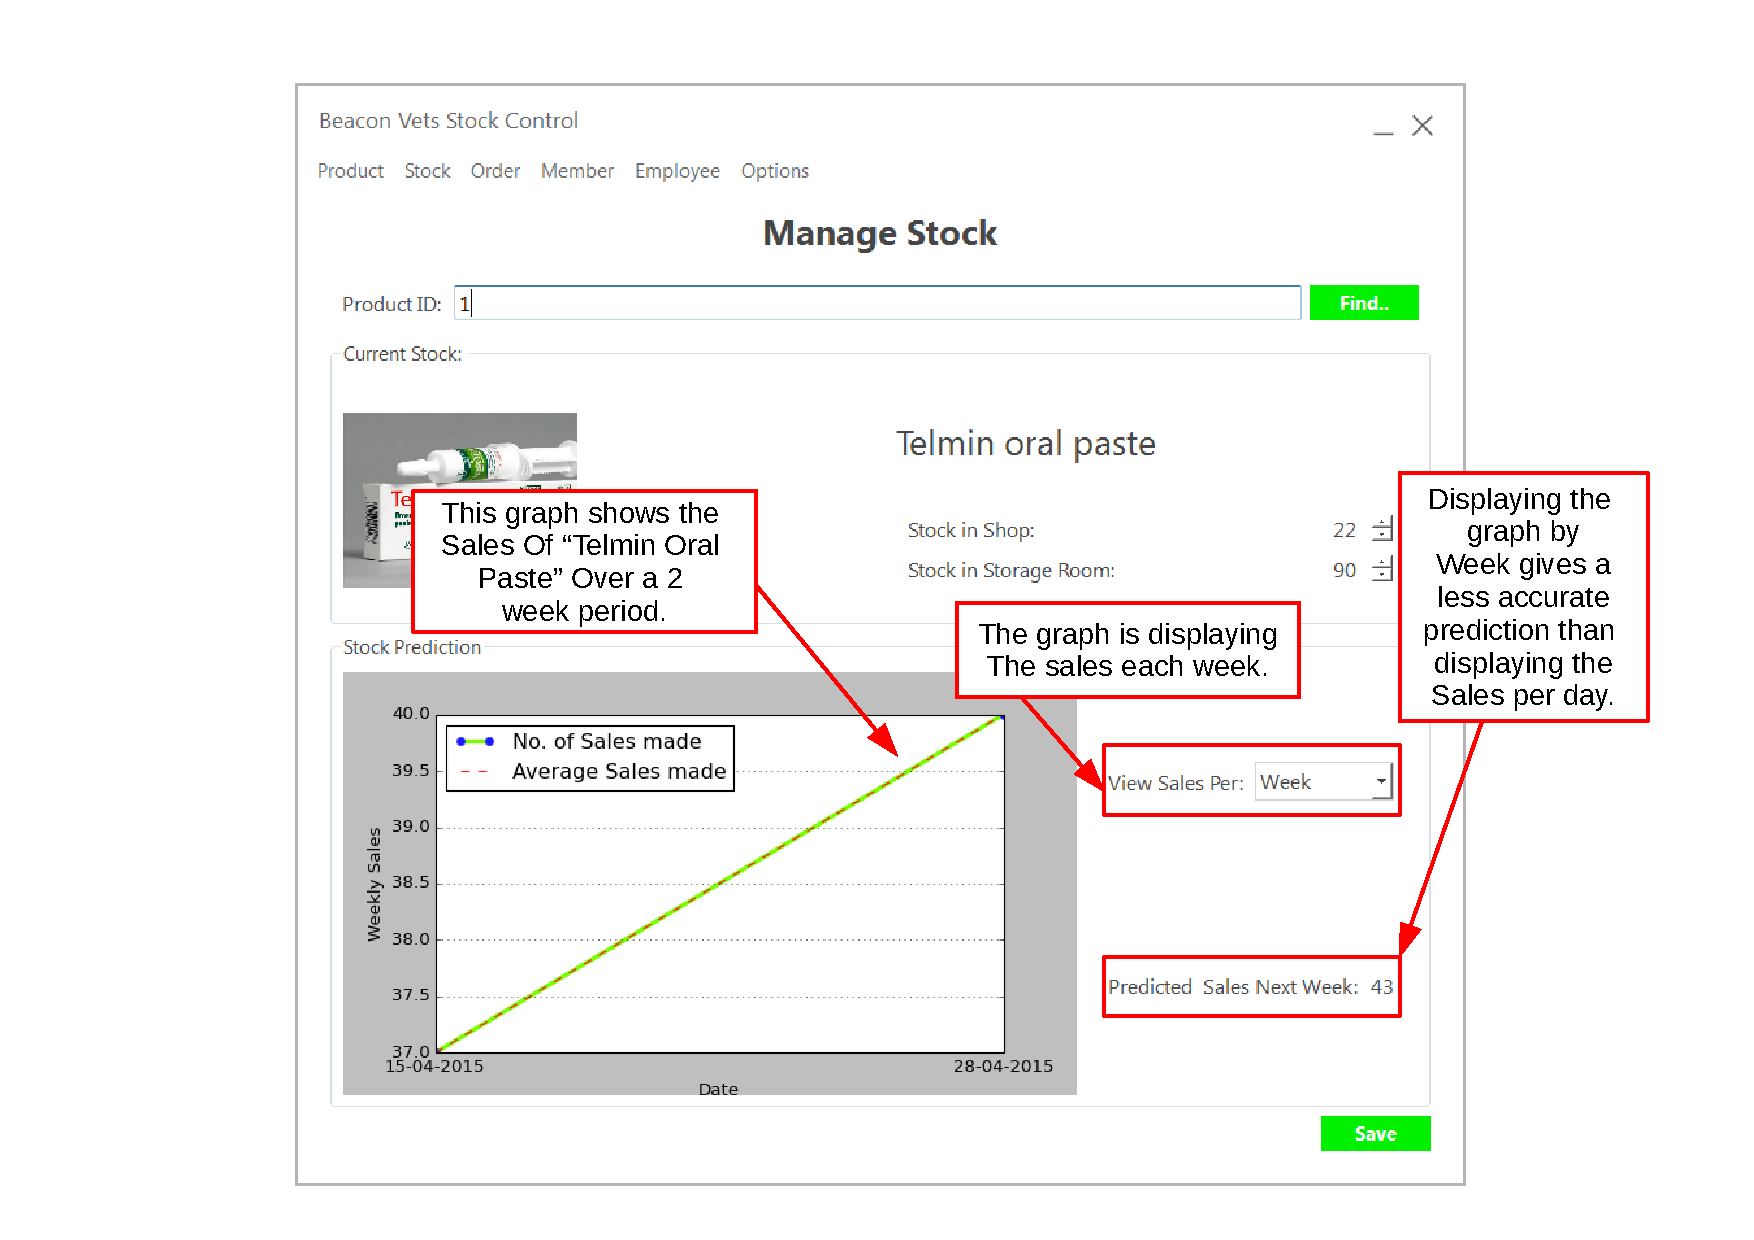
\includegraphics[width = \textwidth]{./Evaluationimages/graph-evidence-1.pdf}
\end{figure}

\begin{figure}[H]
\caption{Graph displaying daily sales of a product} \label{fig:graph-evidence-2.pdf}
\hfill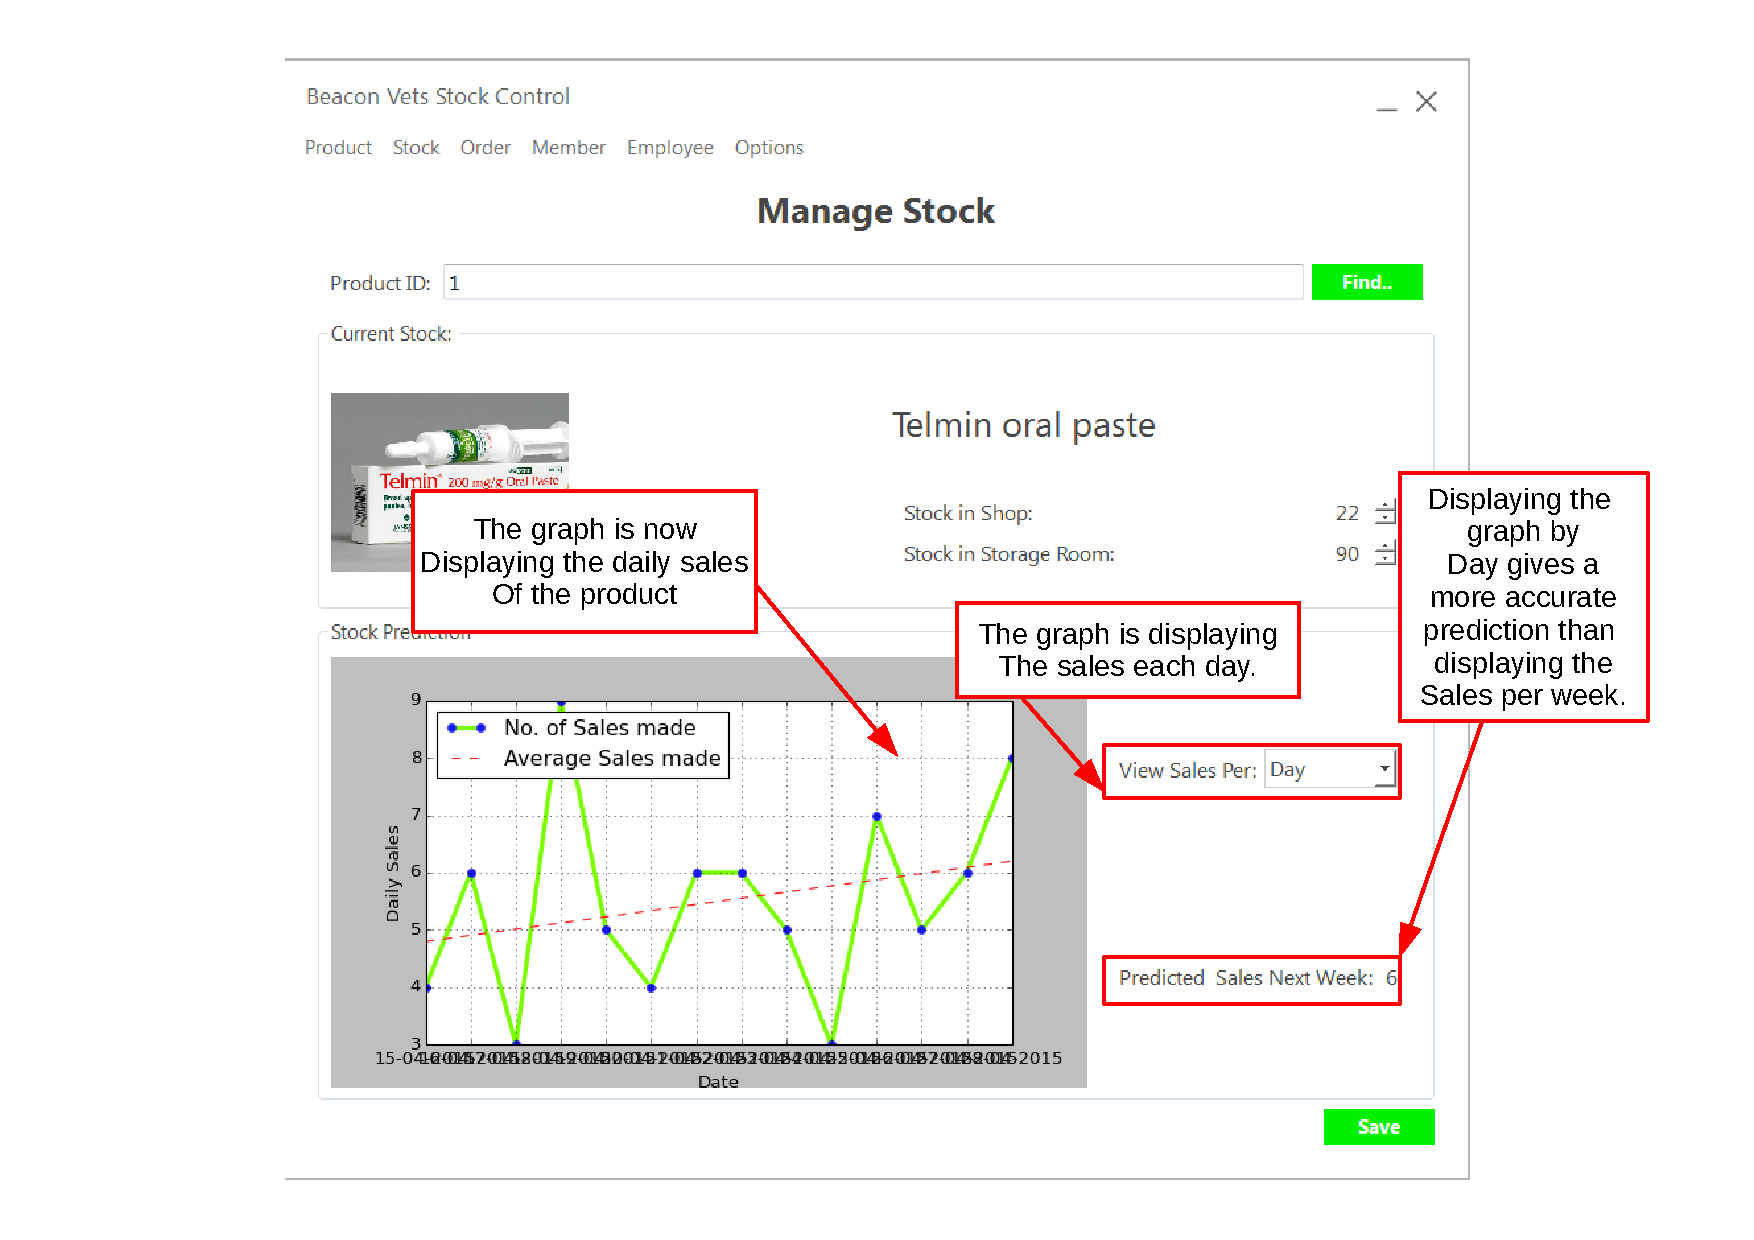
\includegraphics[width = \textwidth]{./Evaluationimages/graph-evidence-2.pdf}
\end{figure}




\pagebreak
\subsubsection{-For the MemberID to be entered and the identity of the client is confirmed to make sure they are a member.}

\textbf{Was the Objective Fulfilled?} \newline

\textbf{\large{This objective was fulfilled}}

When the user wants to edit a member in the system they must enter the MemberID of each member. If the member is in the system their information will be displayed to the user, if not, then the user is told that the Member is not currently in the system. This process is done automatically when the user enters a MemberID into the creating order interface, it will either apply a 10 percent discount if the Member is stored in the system and will not apply it if they are not in the system.

\pagebreak

\textbf{Evidence} \newline

\begin{figure}[H]
\caption{Evidence that the the MemberID is checked against the system to confirm they are a member} \label{fig:evaluation-12-1}
\hfill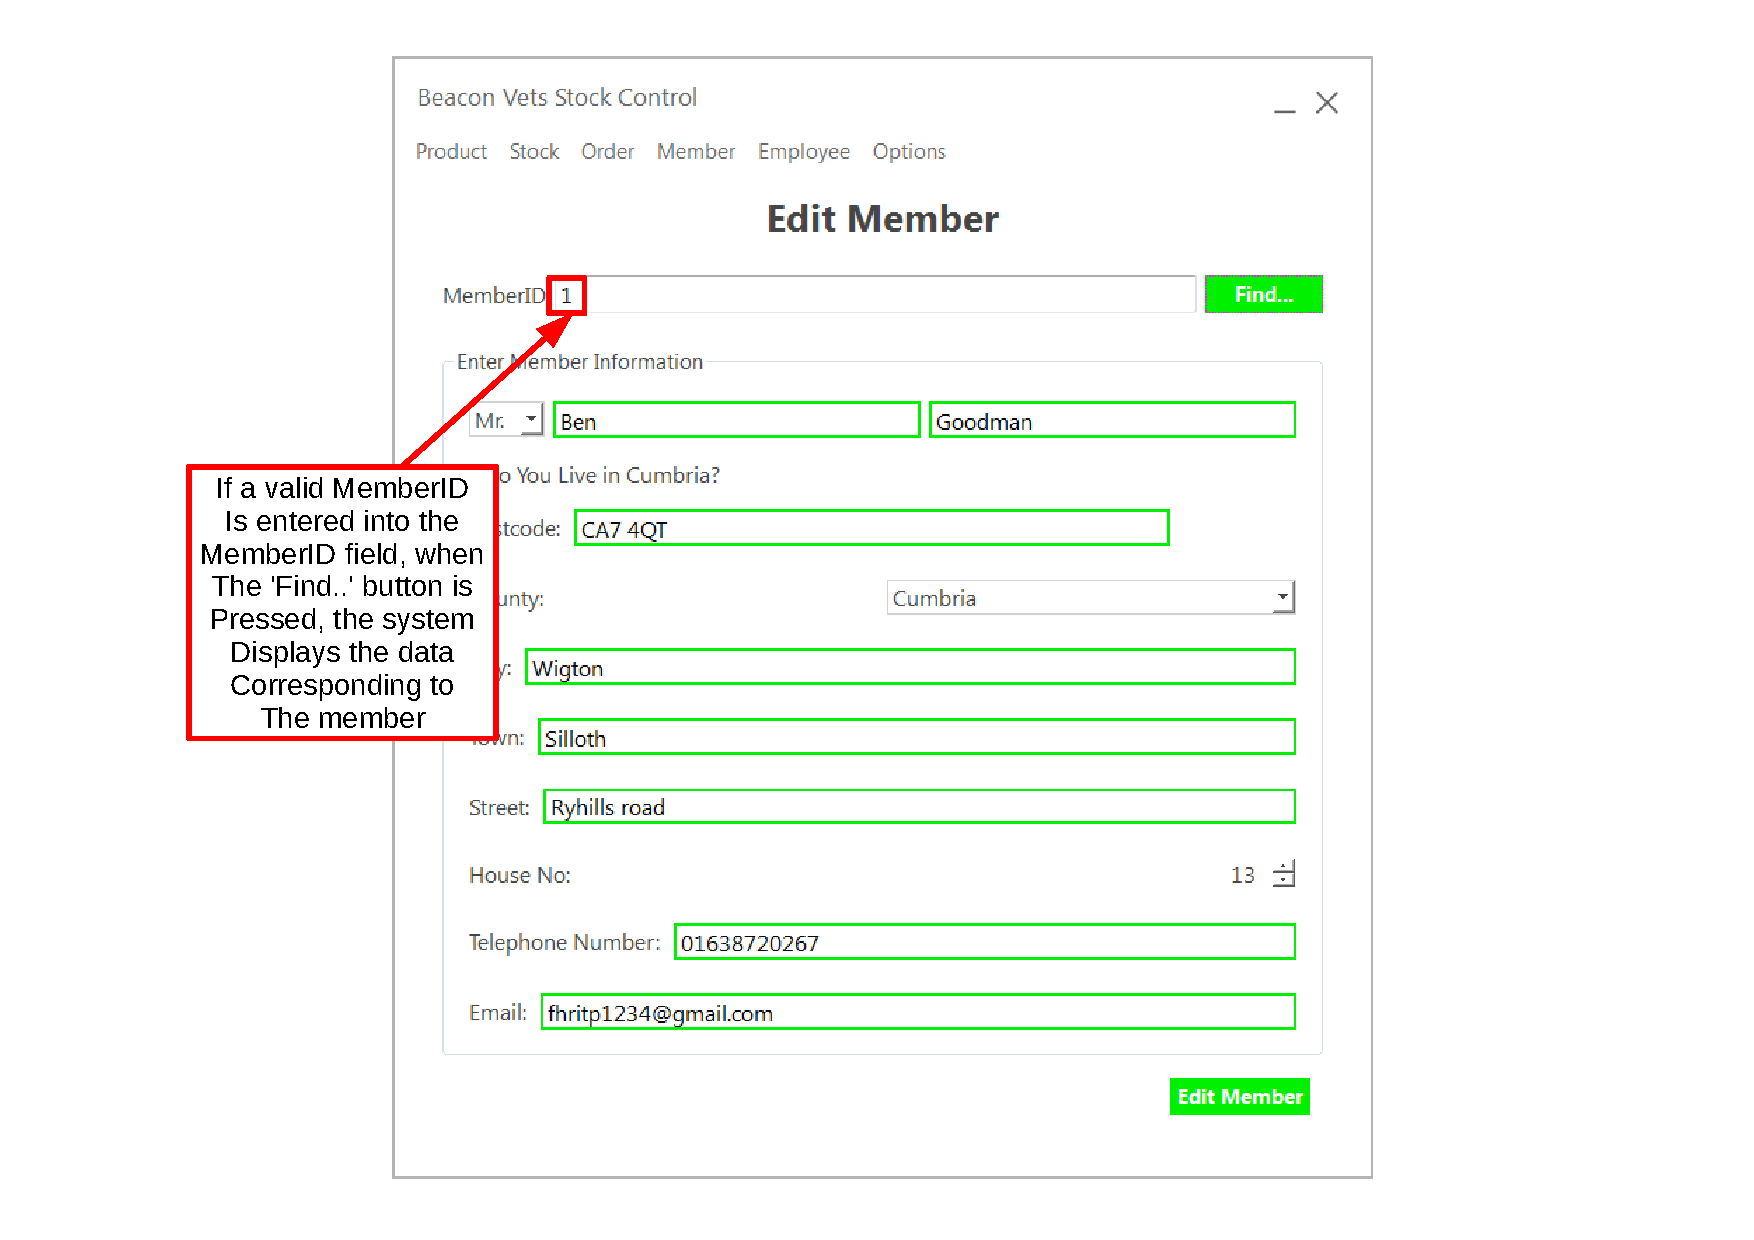
\includegraphics[width = \textwidth]{./Evaluationimages/evaluation-12-1.pdf}
\end{figure}

\begin{figure}[H]
\caption{Evidence that the the MemberID is checked against the system to confirm they are a member} \label{fig:evaluation-12-2}
\hfill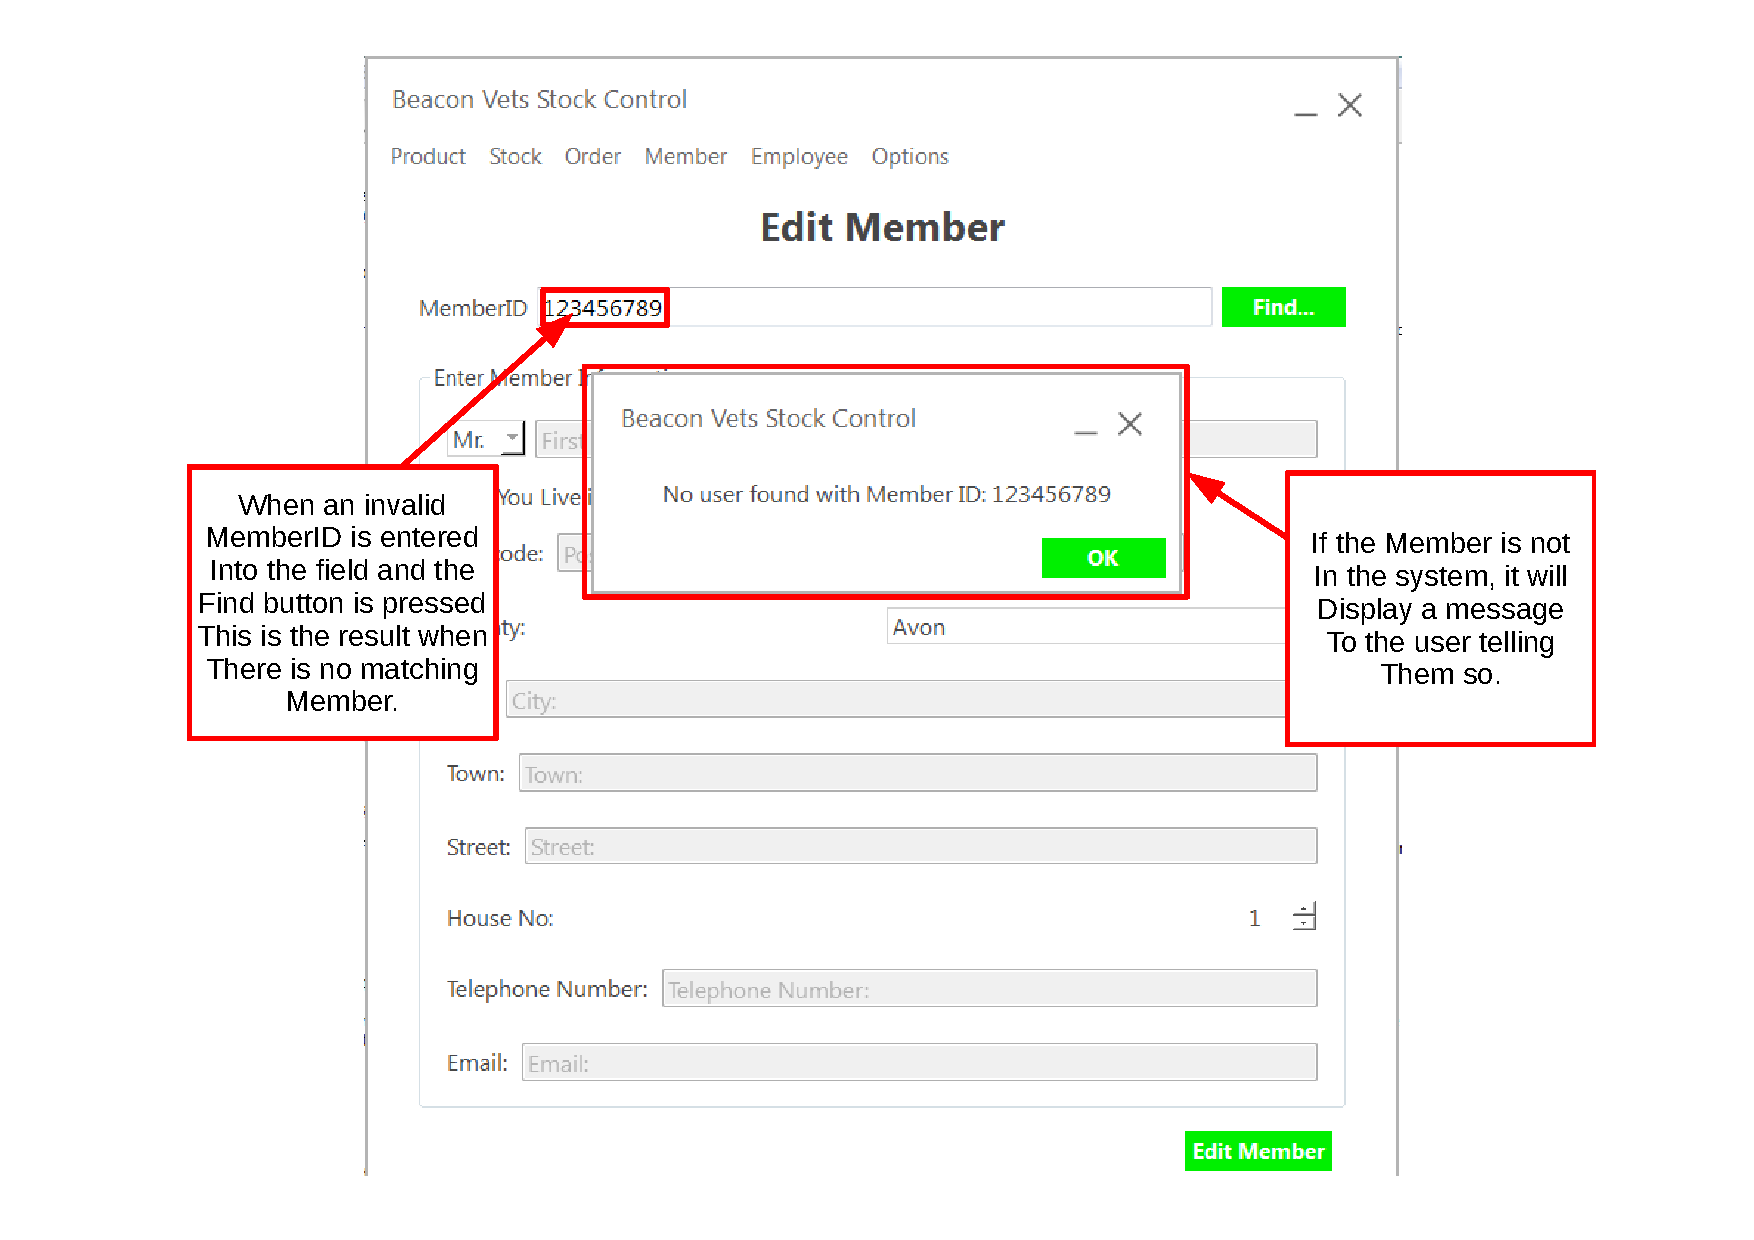
\includegraphics[width = \textwidth]{./Evaluationimages/evaluation-12-2.pdf}
\end{figure}






\pagebreak
\subsubsection{-For Keyboard Shortcuts to be available for the system to be accessed faster.}
\textbf{Was the Objective Fulfilled?} \newline

\textbf{\large{This objective has been fulfilled}}

A large variety of keyboard shortcuts have been produced for the system to make the flow of control much faster. The keyboard shortcuts use relevant keys, relating to there function. For example to \textbf{A}dd a product tot he system, the user can press CTRL and \textbf{A}. 

\textbf{Evidence} \newline

This objective was evaluated during the implementation stage. I ensured that the keyboard shortcuts functioned correctly, and gave the users the oppotunity to highlight any outlined issues in Question 10 of the questionnaire. None of the users said that there were any problems with the shortcuts, however, they did provide improvements that could be made. The main improvement highlighted by the users were that more keyboard shortcuts should be provided for other ares of the system. Question 10, regarding the keyboard shortcuts in the system, allowed me to see how many users actually used the keyboard shortcuts and how many did not.

The pie chart below shows the users that did and didn't use the keyboard shortcuts.

\begin{figure}[H]
\caption{Comparison between the users who did and did not use the keyboard shortcuts in my system} \label{graph4}
\hfill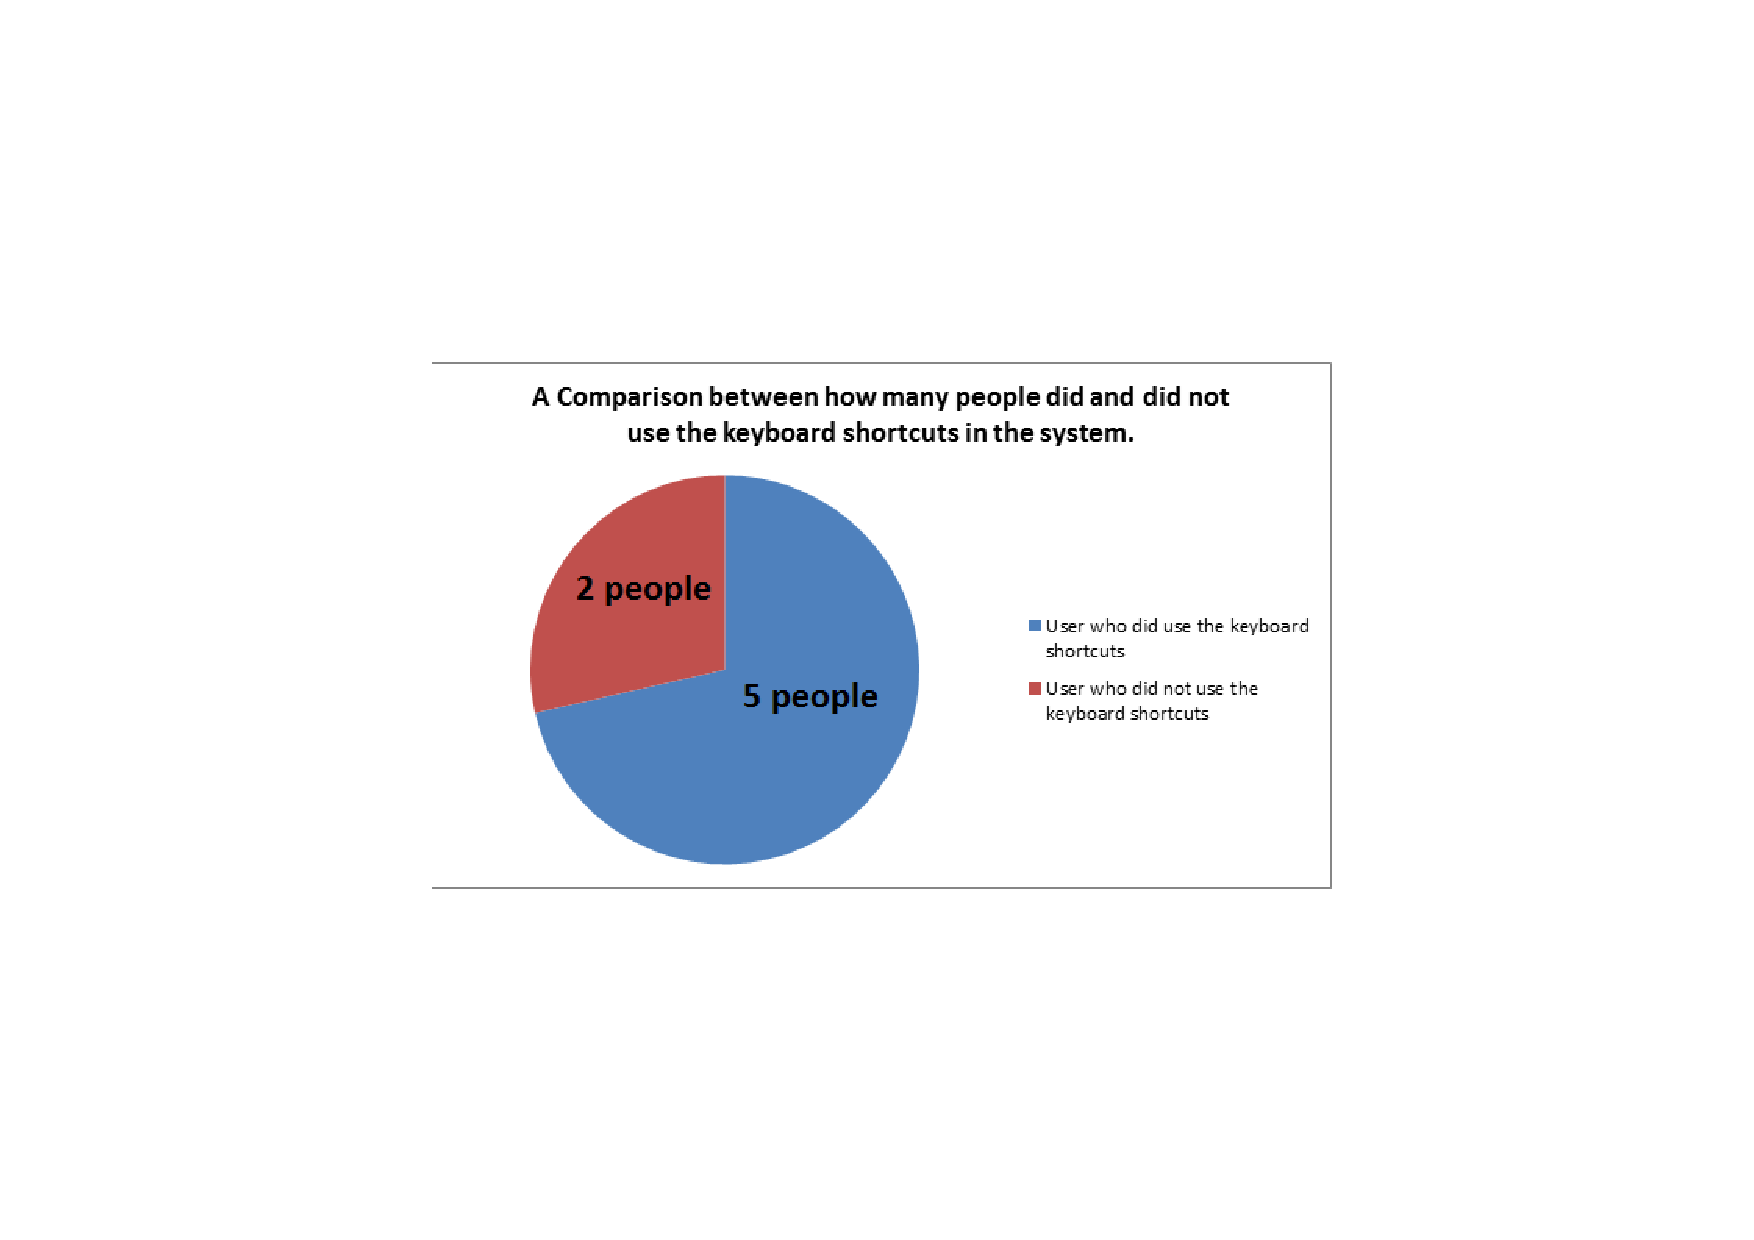
\includegraphics[width = \textwidth]{./Evaluationimages/graph4.pdf}
\end{figure}

From figure \ref{graph4} above, i can see that 5 users used the keyboard shortcuts and 2 users who did not. From this, i can conclude that the keyboard shortcuts were available for the users to use and gives some evidence that the other users of my system (other than my client), have a more than basic knowledge of computers. The 5 people who used the keyboard shortcuts evidences that they are available to use in the system, and by using the keyboard shortcuts myself, can conclude that they allow you to navigate the system a lot faster than using the mouse. Therefore, i can conclude this objective has been fulfilled.


\pagebreak
\subsubsection{-To Format a well structured receipt that is easy for the customer to read and to understand}
\textbf{Was the Objective Fulfilled?} \newline

\textbf{\large{This objective has been fulfilled}}

The invoice for an order has been created using HTML. The top left hand corner of the invoice displays the company logo and location and contact information. The invoice also displays the customer the invoice is due to along with all the products in the order along with their price. The invoice also creates a date and time the invoice was created and sent. The products are displayed in a table to make them easy to read for the customer.

\textbf{Evidence} \newline

The image below shows what the invoice looks like. The information in the top left hand corner is the company info and all the other information is unique to the invoice.

\begin{figure}[H]
\caption{Example of an invoice} \label{invoice}
\hfill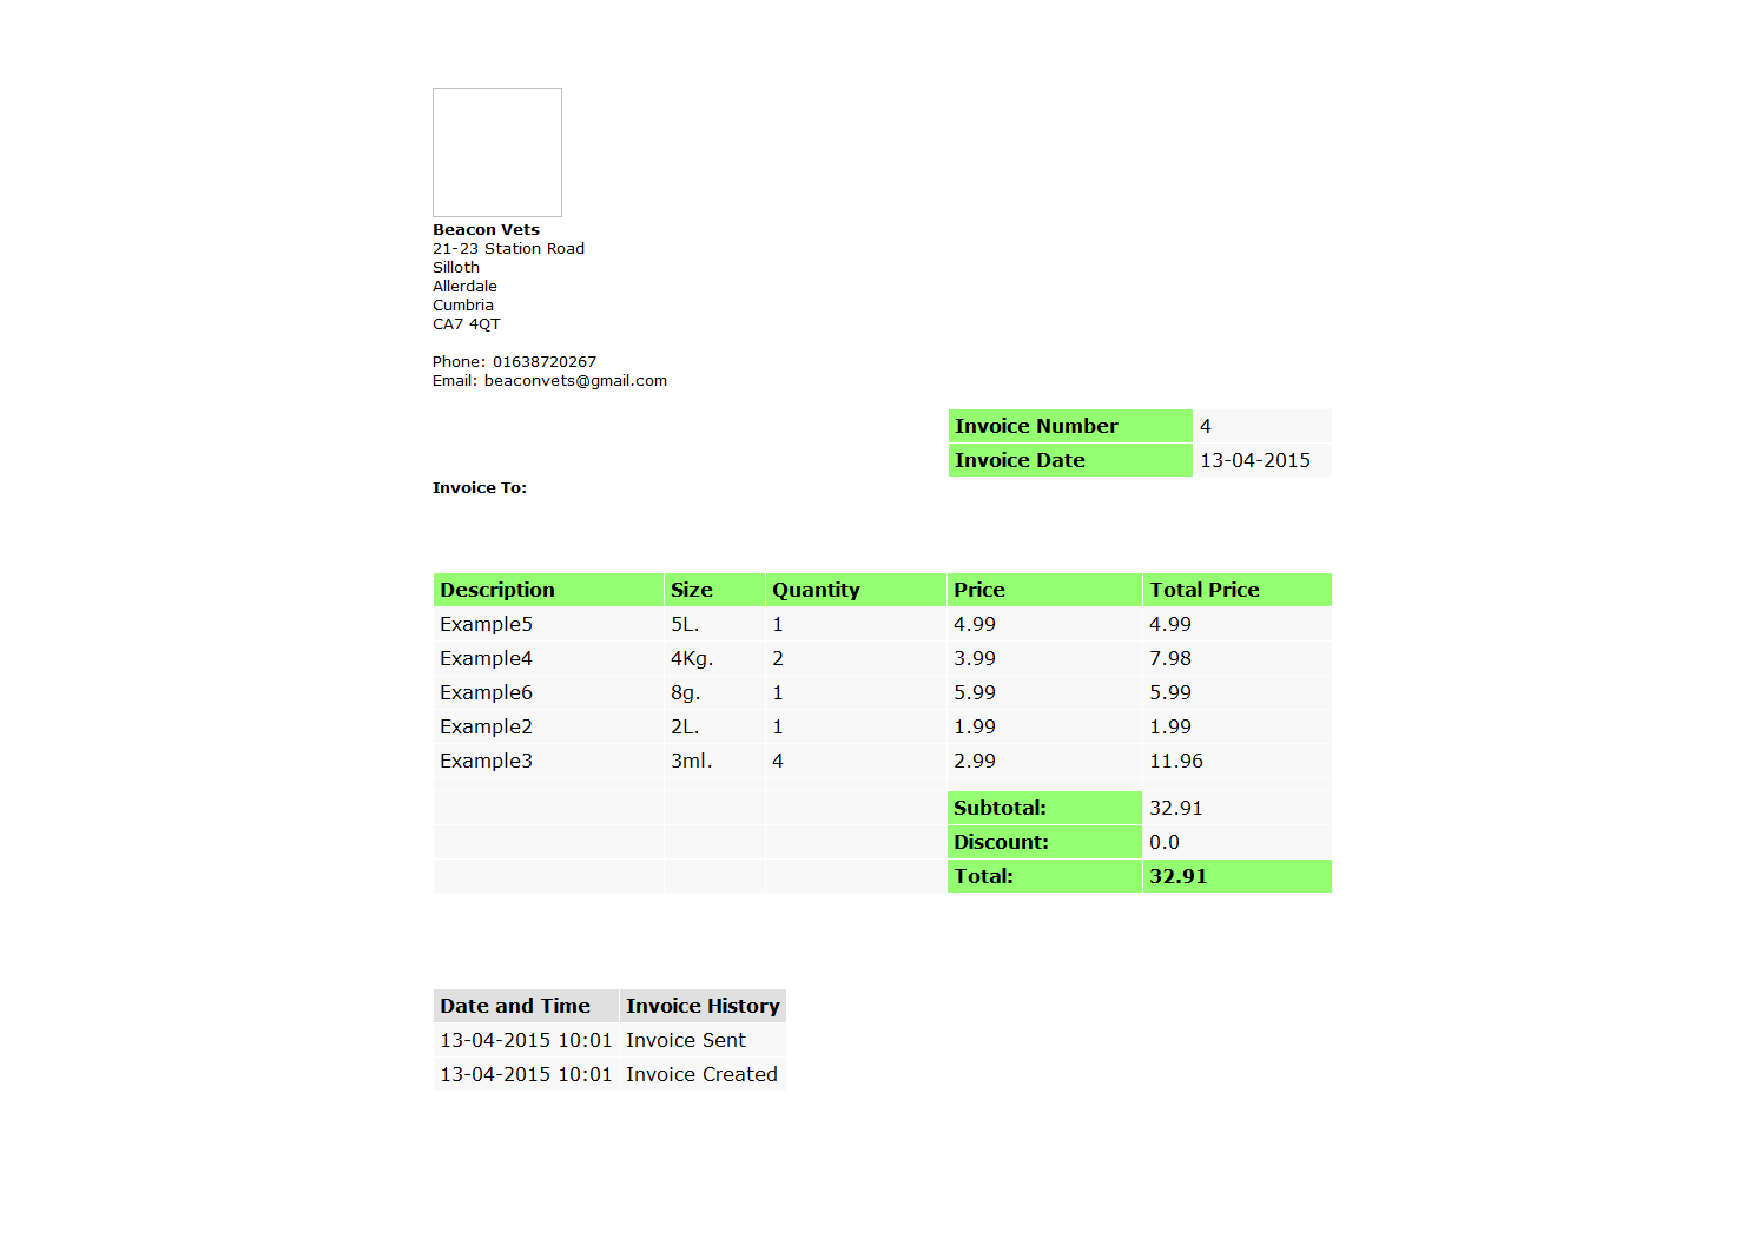
\includegraphics[width = \textwidth]{./Evaluationimages/invoice.pdf}
\end{figure}

\pagebreak

Question 11 of the questionnaire asked the users, "How well was the invoice structured" and had to choose an option between the range of 1 and 5 where 5 was exceptional and 1 was aweful. The graph below shows the results from the questionnaire.

 \begin{figure}[H]
\caption{A Graph to show the users opinion on the structure of my invoice} \label{graph5}
\hfill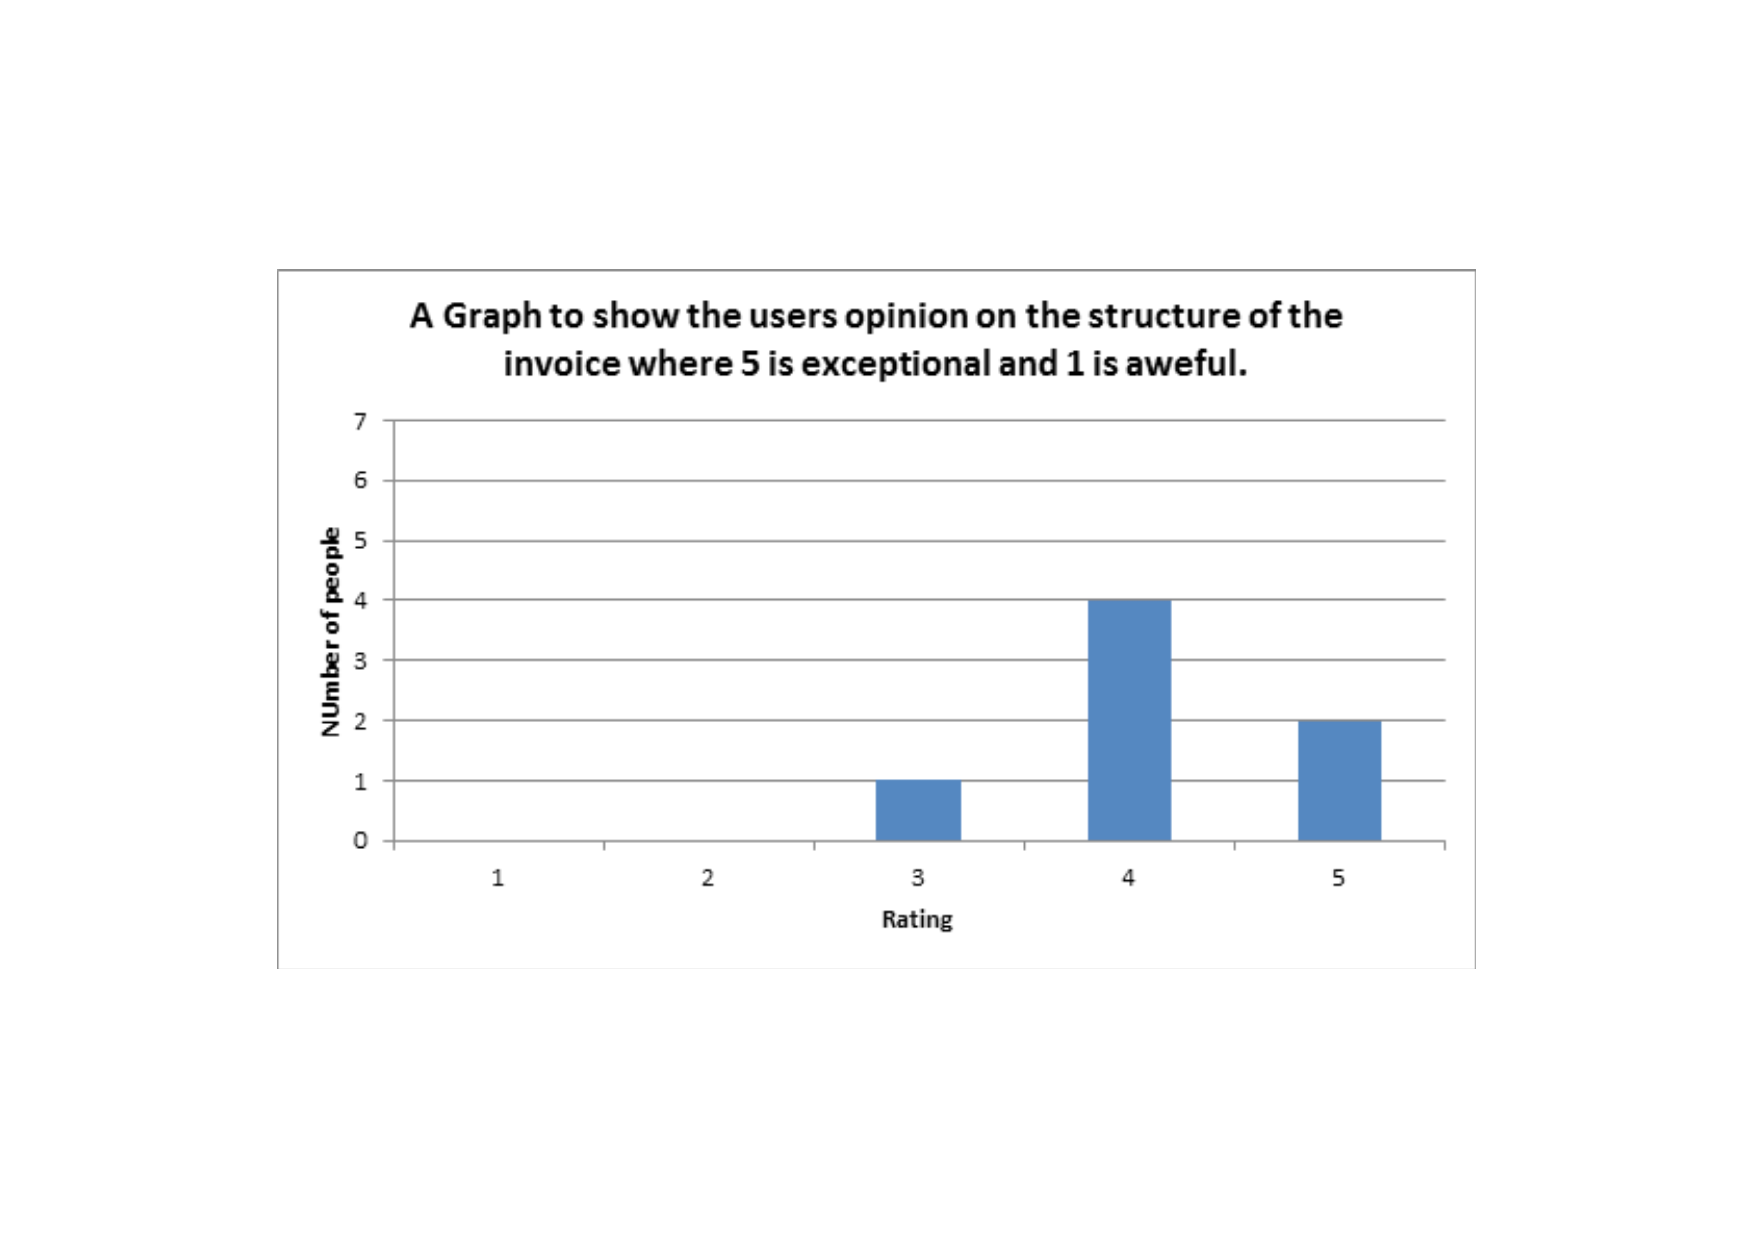
\includegraphics[width = \textwidth]{./Evaluationimages/graph5.pdf}
\end{figure}

From this graph, i can see that generally, the users of the system were happy with the structure of the invoice, 6 of the 7 users giving a rating of 4 or 5, meaning the structure is very good. The users were also asked in Question 11, any improvements that could be made to the invoice. Below i have listed the improvements suggested by all 7 users.

\begin{itemize}
	\item{ Make the Text easier to read}
	\item{ Make the font size larger}
	\item{ Change the colour scheme}
	\item{Implement the functionality to track the invoices}
\end{itemize}

These Improvements were suggested in Question 11, Question 14 and Question 15 in Questionnaire 1 on page \pageref{Client-Q1}, Question 14 and Question 15 in Questionnaire 3 on page \pageref{Questionnaire3}, Question 11 and Question 14 in Questionnaire 3 on page \pageref{Questionnaire3}. Question 11  in Questionnaire 5 on page \pageref{Questionnaire5}, Question 15  in Questionnaire 6 on page \pageref{Questionnaire6} and Question 11 and Question 15 in Questionnaire 7 on page \pageref{Questionnaire7}.


These changes could be made to the invoice in a future version of the system, to improve upon the structure of the invoice.

In the Questionnaire given to my client, I asked them; "To what extent do you agree that the objective has been met". My clients response can be found on page \pageref{Client-Q11}, however i have also provided a word process version in Figure \ref{response1} below, of the response, as my clients handwriting is difficult to interpret.

 \begin{figure}[H]
\caption{The Word Processed version of my clients response to Question 11 of the Questionaire} \label{response1}

\vspace{3mm}
\textit{\large{"I Partially agree as i can clearly understand the information on the interface, however, i do not like the colour scheme and the font should be changed so that it is easier to read"}}
\end{figure}
\vspace{3mm}

My client specifies that they can clearly understand the information on the interface, and also provided improvements that can be made. This evidence, along with the responses from the other users, can conclude that this objective has been fulfilled.


\pagebreak
\subsubsection{-Allowing the Order of the products in the database to be changed.(i.e. Max - Min Price, A-Z ect \ldots)}
\textbf{Was the Objective Fulfilled?} \newline

\textbf{\large{This objective has been fulfilled}}

On every table within my system. The user has the ability to click on a column heading and the contents of the table will be sorted by that column. For example, by default all the products will be sorted by their ProductID's. If the user clicks on the price column heading the products will be sorted by price, lowest to highest. If the user then clicks on the price column header again, it will sort the products by price highest to lowest.

This objective was fulfilled during the Implementation stage. During the Implementation stage i ensured the algorithm used to organise the items in the table functioned correctly. I provided the users with an area to provide feedback on any problems in Question 12 of the questionnaire. No users reported any problems when organising the data which implies that this area of the system functions correctly. This evidence concludes that this objective has been met.

\textbf{Evidence} \newline

\begin{figure}[H]
\caption{Default order of products in the search window.} \label{new-evaluation-1}
\hfill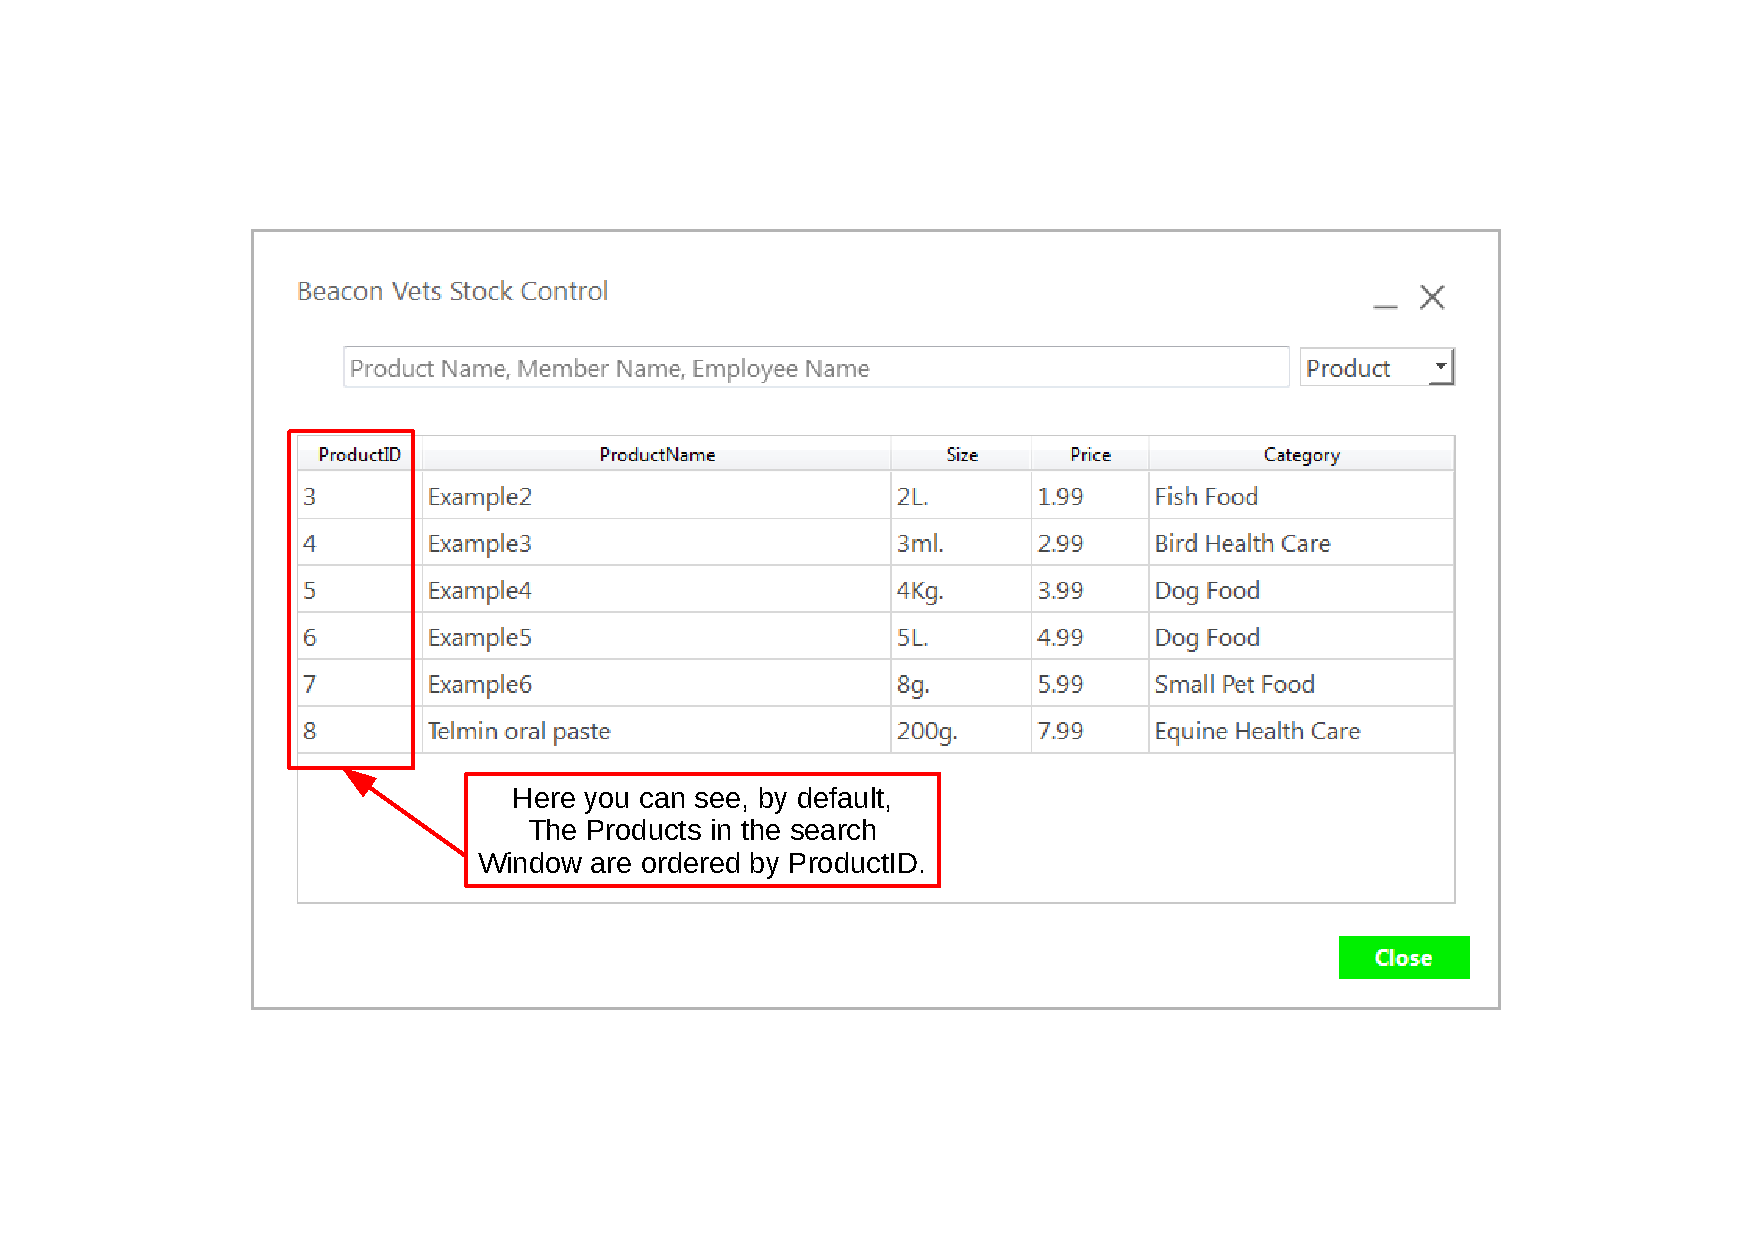
\includegraphics[width = \textwidth]{./Evaluationimages/new-evaluation-1.pdf}
\end{figure}

\begin{figure}[H]
\caption{Order of products in the search window by descending ProductID.} \label{new-evaluation-2}
\hfill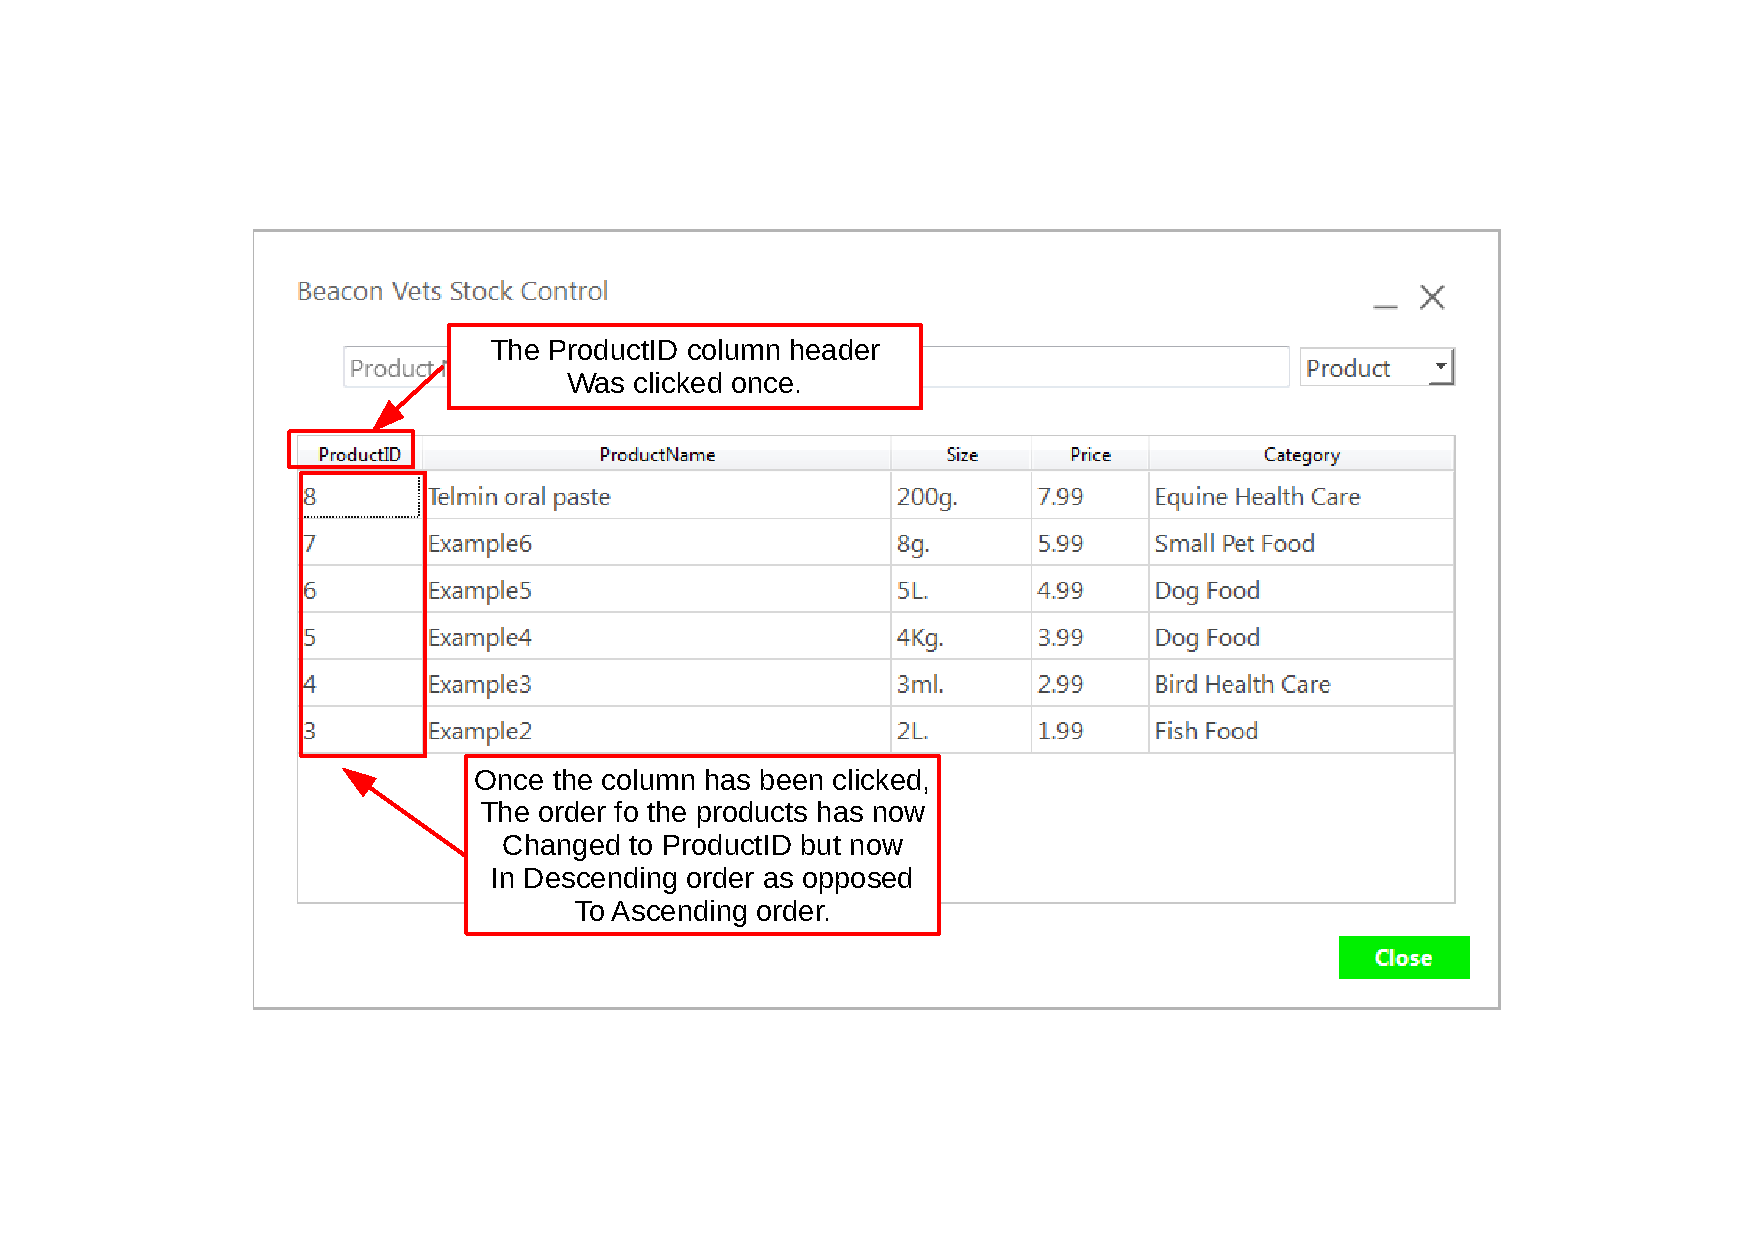
\includegraphics[width = \textwidth]{./Evaluationimages/new-evaluation-2.pdf}
\end{figure}

\begin{figure}[H]
\caption{Order of products in the search window by descending Ascending Price.} \label{new-evaluation-3}
\hfill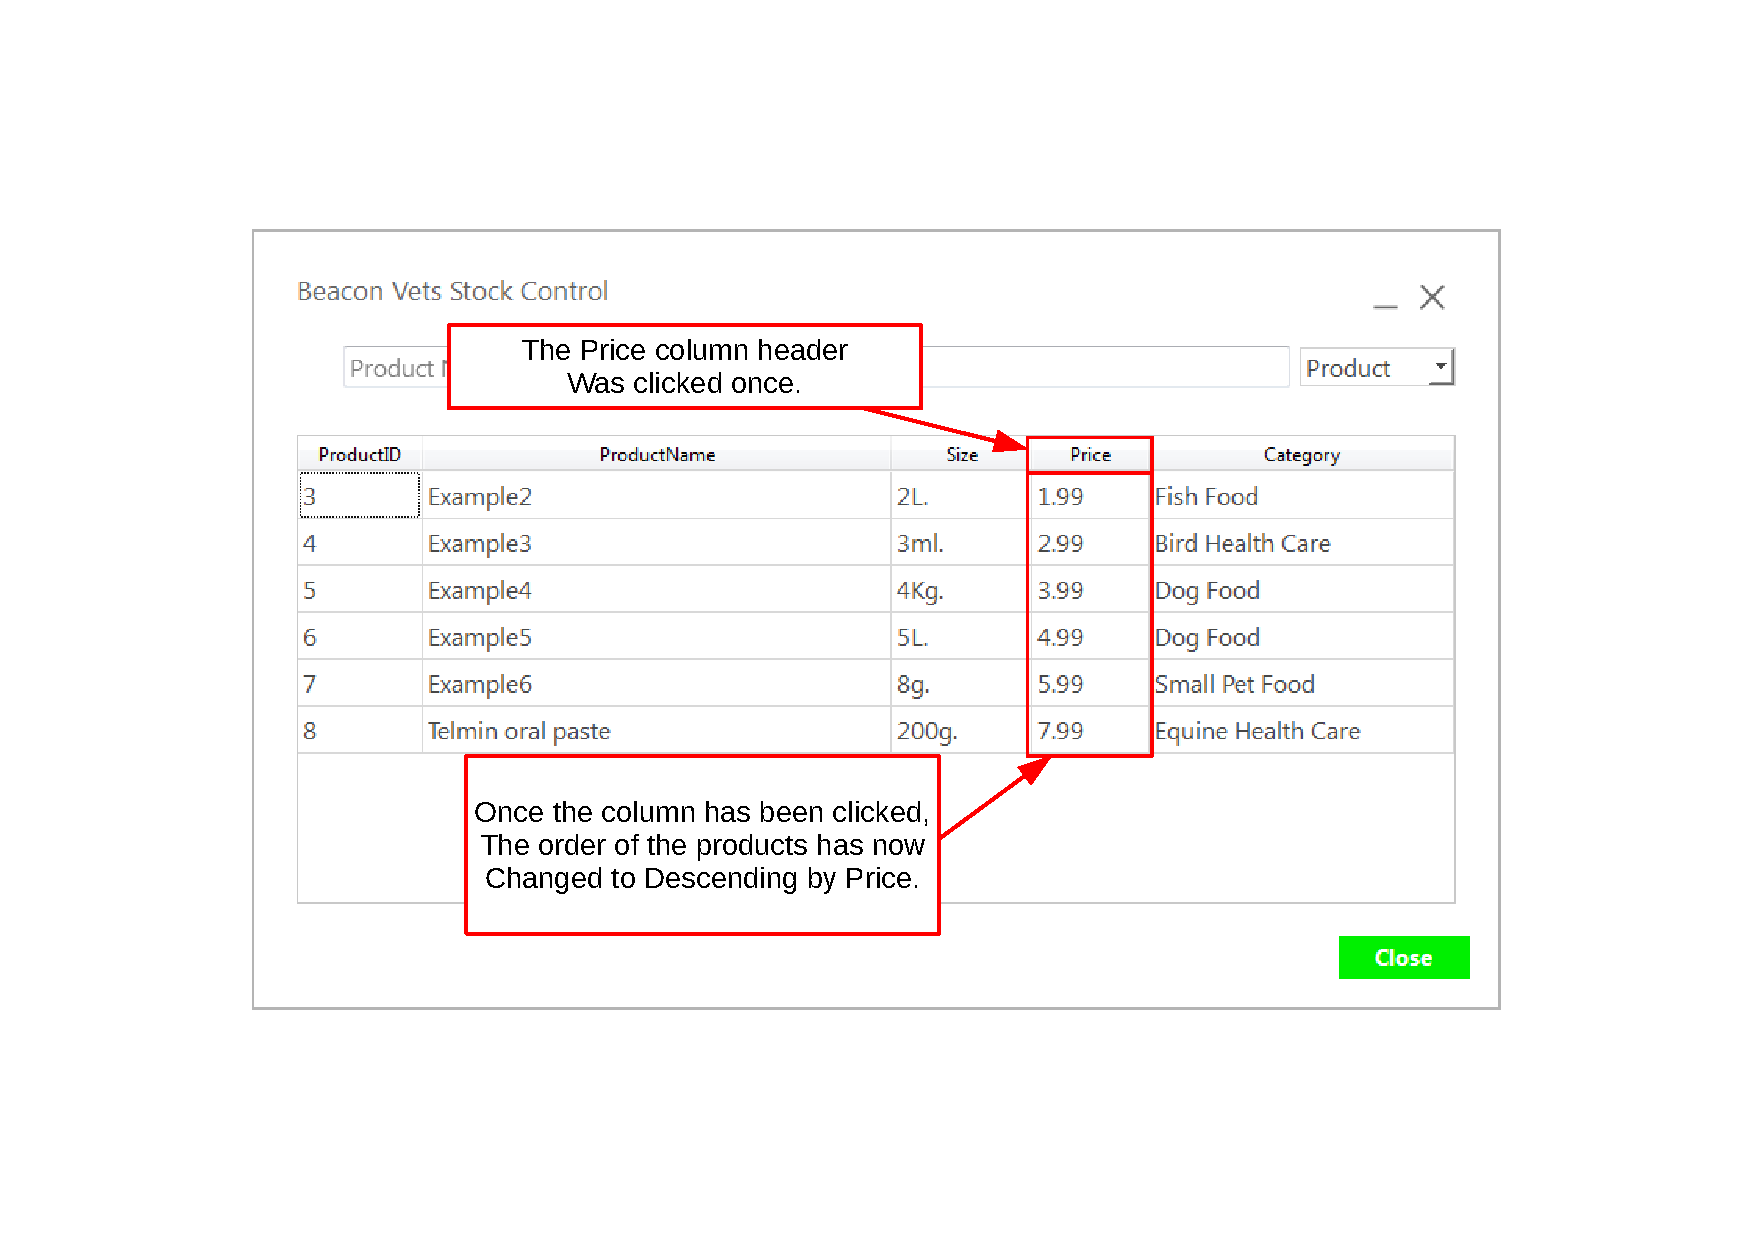
\includegraphics[width = \textwidth]{./Evaluationimages/new-evaluation-3.pdf}
\end{figure}

One of the Options in Question 12, was that the user could select whether or not they actually tried changing the order of the table. The pie chart below shows the people who did and did not use this feature.

\begin{figure}[H]
\caption{Graph to show the people who did and did not re-order the tables.} \label{graph6}
\hfill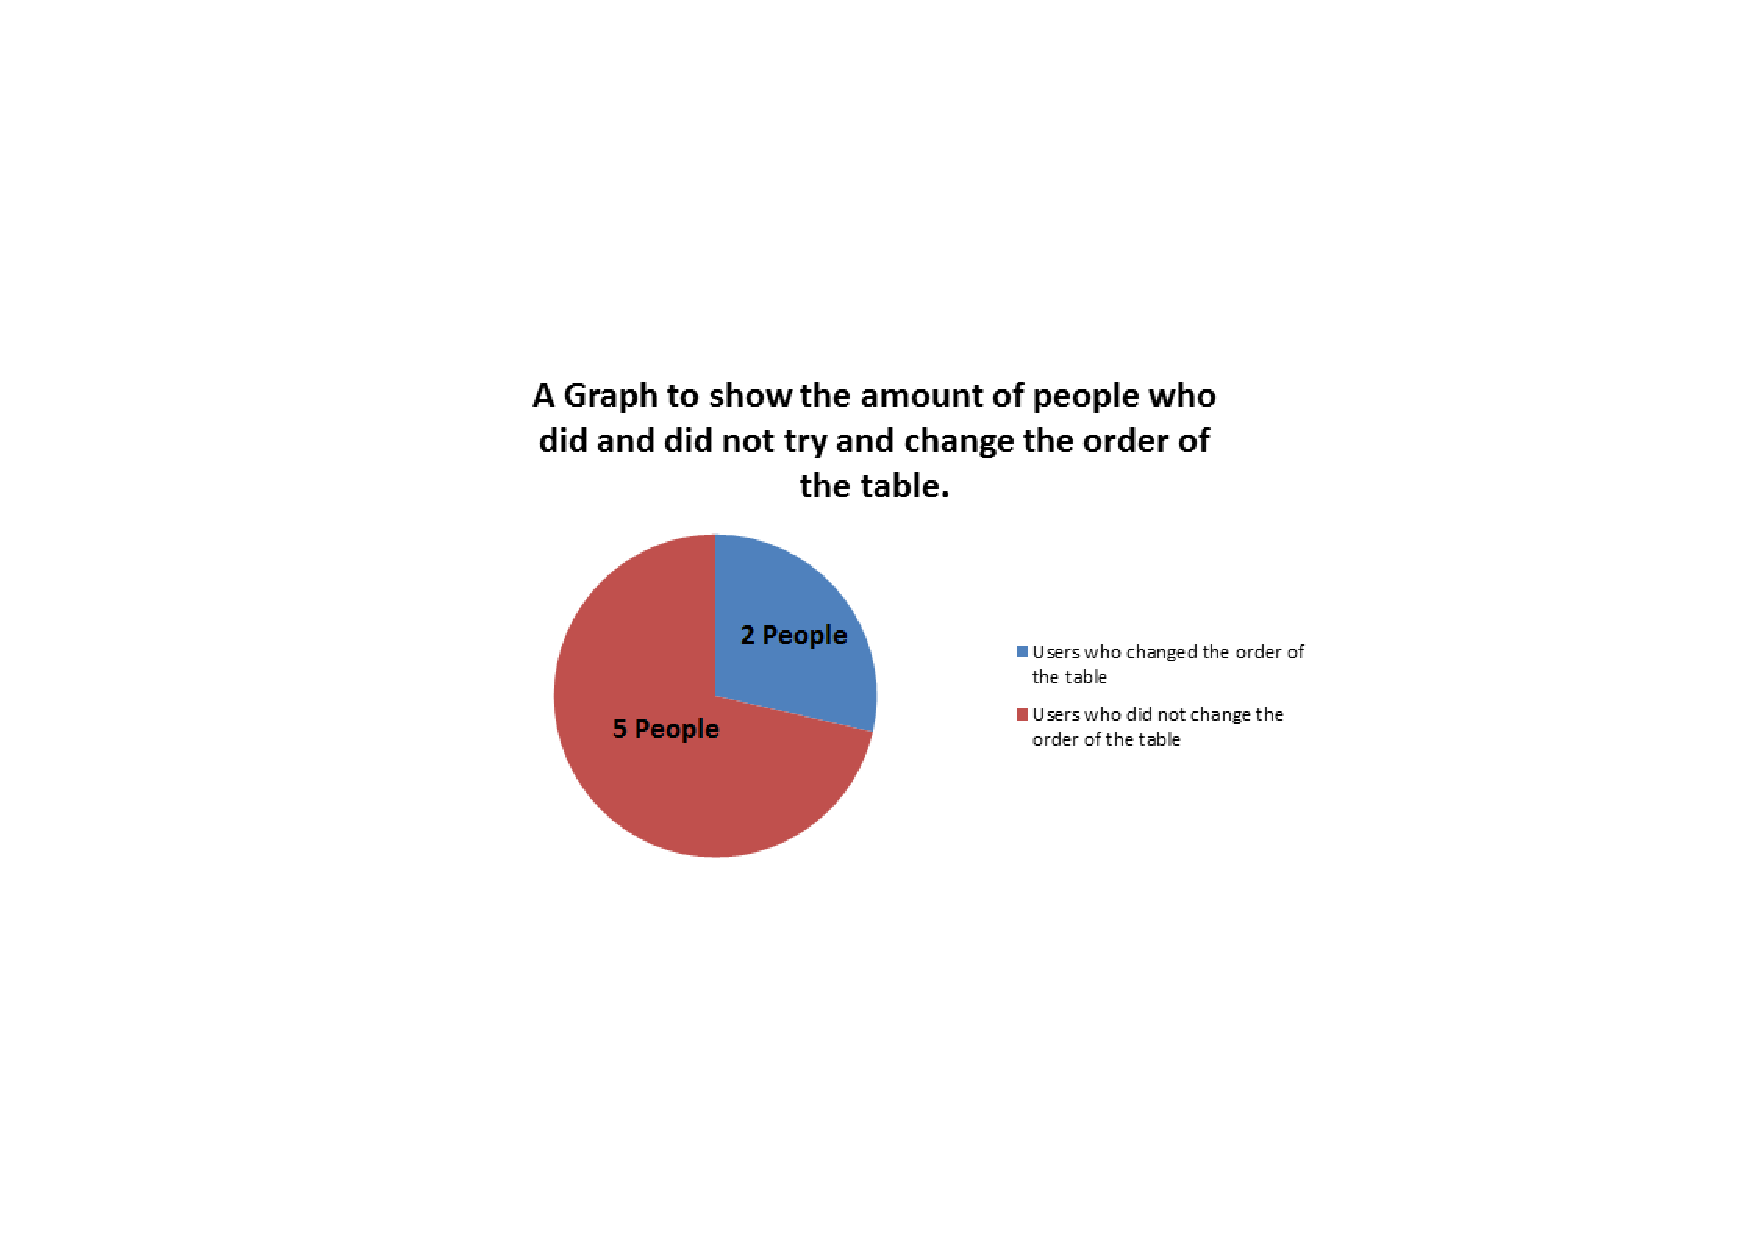
\includegraphics[width = \textwidth]{./Evaluationimages/graph6.pdf}
\end{figure}

This graph shows that only 2 of the 7 people actually changed the order of the table. This provides evidence, that if there are any problems with the ordering of the data that were not discovered during the testing phase, may still be present because very few people actually used this feature. However, this is quite unlikely as this was a fairly easy feature to implement with little margin for error.

The fact that 5 of the 7 users did not change the order of the table may be due to them not knowing the system could do it. This could have been improved by giving a more in-depth tutorial to each individual user. This would increase the chance of any unknown problems to be identified.

















\pagebreak
\section{Effectiveness}

\subsection{Effectiveness of General Objectives}

\vspace{10mm}

\subsubsection{-Data can added to the database easily}

\textbf{Effectiveness Criteria:}\newline
\begin{itemize}
	\item{The data fields should be organised and grouped together into a group box}
	\item{Validation should be clear so the user knows when data is or isn't valid}
	\item{Drop down menus will be available where possible to reduce the amount of erroneous data.}
	\item{Each data field and button should be self explanatory, for example, the 'Save' button should save the data.}
\end{itemize}
\textbf{Judgement and Evidence:} \newline

\textbf{\large{This objective has successfully been met}}

All of the data input fields have been organised inside group boxes and all of the data fields have been labelled to make them self explanatory and all the buttons are self explanatory. Below i have provided evidence of this:

I have used drop down menus where possible, for example for the Counties and Name Title when adding a member. The Validation displays a bright green boarder around the the data field which i feel is clear, however, my client may not know why the data is or is not valid.

Referring to the Question 1 of my questionnaire, all of the users who tested my system, did not find the process of adding data to the database hard. figure \ref{graph1} on page \pageref{Graph1} shows a bar graph of how easy each user found adding data to the system to be.

In the Questionnaire given to my client, i asked to what extent he agreed that this objective had been met. My client's response can be found on page 




\pagebreak
\subsubsection{-Data can be edited within the system easily.}

\textbf{Effectiveness Criteria:}\newline
\begin{itemize}
	\item{The data should be able to be found easily in the system.}
	\item{The data fields should be organised and grouped together into a group box}
	\item{Validation should be clear so the user knows when data is or isn't valid}
	\item{Drop down menus will be available where possible to reduce the amount of erroneous data.}
	\item{Each data field and button should be self explanatory, for example, the 'Save' button should save the data.}
\end{itemize}

\textbf{Judgement and Evidence:} \newline

\textbf{\large{My solution has been effective}}

 My edit data interfaces are very similar to my add data interfaces, therefore items 2-4 have been met. I feel I have partially met the criteria of "The data should be able to be found easily in the system." i have created a search window which allows the user to search for the data they want to edit. The user can also go straight to the edit interfaces from the search table, by right clicking the item they want to edit and clicking on the edit button from the right click drop down menu. However, I feel that a more effective solution to this objective could be to include a small drop down menu of all the members in the system where the user can simply select an existing member from the drop down menu. The results from my questionnaire have shown that my client and other users of the system found my current solution to be effective. For evidence, see question 2 of the Questionnaires found in the `Questionnaires' section.





\pagebreak
\subsubsection{-Easy to understand the layout of the information.}

\textbf{Effectiveness Criteria:}\newline
\begin{itemize}
	\item{All QLineEdits should have QLabel to explain what data should be displayed or input into the data field.}
	\item{The structure of each interface has been planned, so that the data has been grouped appropriately.}
	\item{All text is easy to read with ease, meaning the size of the font of all text is sufficient.}
\end{itemize}

\textbf{Judgement and Evidence:} \newline

\textbf{\large{My solution has been partially effective}}


Most but not all QLineEdits have been labelled, however some data fields use the place-holder text to describe what data should be entered. This is not the most effective method because the place-holder text cannot be seen once data has been entered into the field. I feel that my solution to the objective has been partially met. Minor changes can be made so that all data fields have a QLabel describing the data that should be entered into the QLineEidt.









\pagebreak
\subsubsection{-Easy to locate a product within the system.}
\label{fig:search-evidence}

\textbf{Effectiveness Criteria:}\newline
\begin{itemize}
	\item{The system should have an interface in which a user can search for a product member or employee in the system}
	\item{The interface should be simple to use, as it is being used by all users, not just my client.}
	\item{Searching for a product, employee or member should be a fast process.}
\end{itemize}

\textbf{Judgement and Evidence:} \newline

\textbf{\large{My solution has been effective}}

My solution, was to create a pop up window, that allowed the user to search the system for either a product, member or employee. The user can choose which one they would like to search for by selecting either `product', `member' or `employee' from a drop down menu. The table will display all of the products members or employees unless the user enters. The feedback in which I received from the questionnaire, showed that my client and all other users of the system found the process of locating a product either easy or very easy. This is shown from Question 3 in my questionnaire.


\subsubsection{-The system as a whole, should be clear and easy to use.}

\textbf{Judgement and Evidence:} \newline

\textbf{\large{My solution has been partially effective}}

From the feedback of my questionnaire, none of the users found the aspects asked about in the questionnaire to be difficult. Therefore, following the results of the questionnaire, i can say that this objective has been fulfilled. Minor improvements could be made which have been specified in Question 14 of the questionnaire. 3 of the users stated that the colour scheme could be improved. Improving the colour scheme will improve the way in which the user can see the data. 



\pagebreak
\subsection{Effectiveness of Specific Objectives}



\subsubsection{-For an image to be displayed when an item is searched for (identifying a product if the Product information is unknown}

\textbf{Effectiveness Criteria:}\newline
\begin{itemize}
	\item{An image is displayed to the user so that they can find products easier}
	\item{The image should be displayed when searching for a product.}
	\item{The image should be able to be changed in the Edit Product interface.}
\end{itemize}

\textbf{Judgement and Evidence:} \newline

\textbf{\large{My solution was not effective}}

I decided to remove this functionality from the system as I caused system instability and caused the system to become unresponsive. For the users who used the search window, they said that no image was displayed, from question 4 of the questionnaire which is as expected. 




\pagebreak
\subsubsection{-For the Stock control system to be integrated with the process of selling items. This is so that the stock is automatically updated when a product is sold.}
\label{stock-change-effectiveness}
\textbf{Effectiveness Criteria:}\newline
\begin{itemize}
	\item{The system should change the stock of each product once an order has been created.}
\end{itemize}

\textbf{Judgement and Evidence:} \newline

\textbf{\large{My solution has been effective}}

Evidence to show that this objective has been fulfilled can be found in figure \ref{fig:evaluation-9-1}, figure \ref{fig:evaluation-9-2} and figure \ref{fig:evaluation-9-3}. Referring to Question 5 of my Questionnaire feedback, 100\% of the users who created orders, found this feature helpful. Therefore, i can conclude that this objective has been met fully.




\pagebreak
\subsubsection{-For the new process of selling products to be quicker, to minimize the time for people queuing.}

\textbf{Effectiveness Criteria:}\newline
\begin{itemize}
	\item{Allow employee to add products to the order easily.}
	\item{for the total price of the order to be calculated automatically}
	\item{for the products to be found easily in the system}
	\item{The system must produce a well structured invoice for each order}
\end{itemize}

\textbf{Judgement and Evidence:} \newline

\textbf{\large{My solution is effective}}

Referring to Question 6 from my Questionnaire, the users did not say they had any problems when creating an order. This suggests that there are no major problems with the creating order interface. The system calculates the price of the order automatically, this is shown in figure \ref{fig:effectiveness-1}. Products being easily found within the system has already been evaluated on page \pageref{fig:search-evidence} and has proven that this objective has been fulfilled. Referring to Question 11 of the questionnaire, the users of the system said that the invoice was well structured. One common comment from the feedback was that the text size of the invoice could be larger and that I could also a different font, such that, the text is easier to read. Therefore, i would say that i have partially met this objective, where improvements to the structure of the invoice could be made to fully meet the objective.

\begin{figure}[H]
\caption{Evidence that the system automatically calculates the price of the order.} \label{fig:effectiveness-1}
\hfill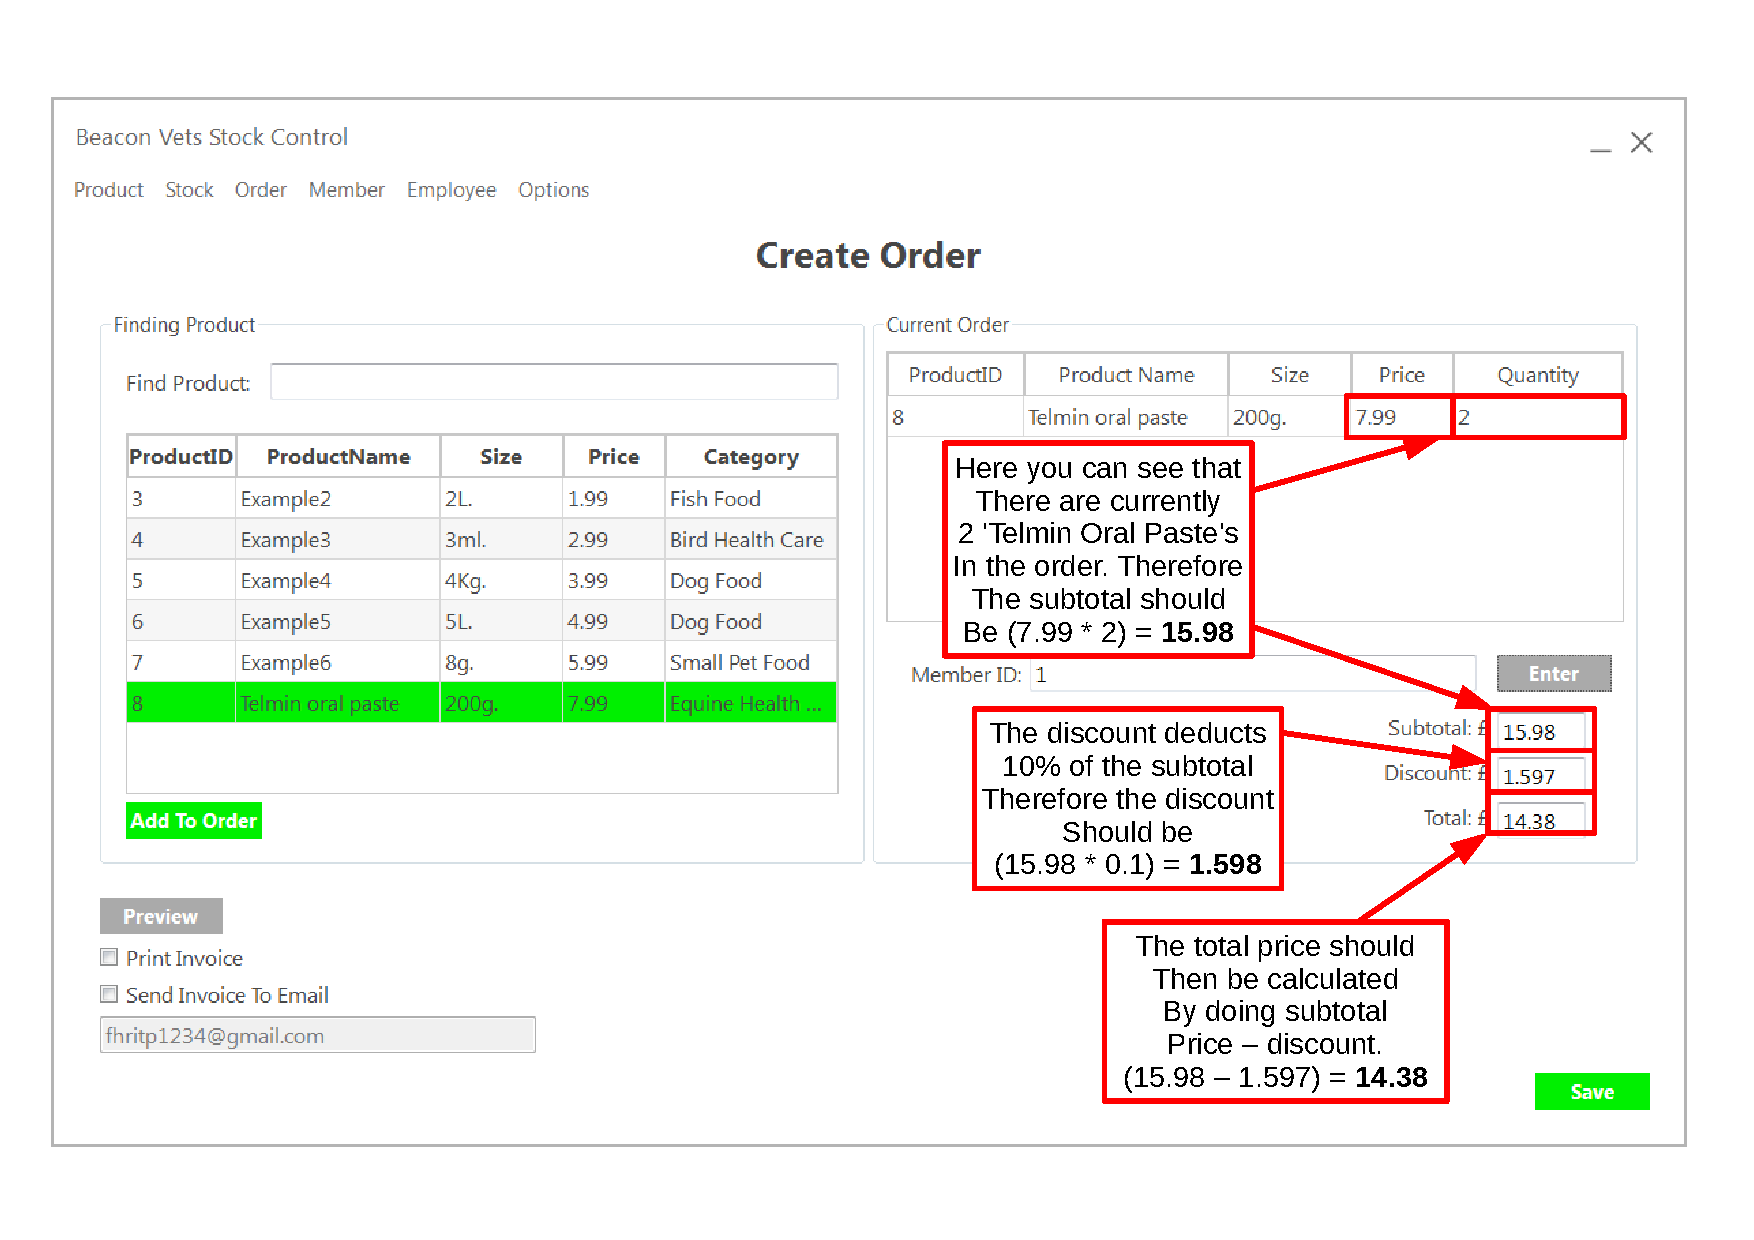
\includegraphics[width = \textwidth]{./Evaluationimages/effectiveness-1.pdf}
\end{figure}





\pagebreak
\subsubsection{-For the current stock to automatically update when the products are bought}

\textbf{Effectiveness Criteria:}\newline
\begin{itemize}
	\item{When a certain quantity of a product is bought, this deducted from the stock of the product when the order is created.}
\end{itemize}
\textbf{Judgement and Evidence:} \newline

\textbf{\large{My solution is effective}}

This objective has already been evaluated for its effectiveness on page \pageref{stock-change-effectiveness}. It was concluded that this objective had been fulfilled fully.



\pagebreak
\subsubsection{-For a reminder message to pop up when stock needs to be moved from storage to the front of the vets. }

\textbf{Effectiveness Criteria:}\newline
\begin{itemize}
	\item{The message should display if the stock of a product falls below a certain amount}
	\item{A message should display if stock needs to be moved between locations.}
\end{itemize}

\textbf{Judgement and Evidence:} \newline

\textbf{\large{My solution is partially effective}}

Referring to question 7 of the questionnaire the users of my client said that this feature functioned properly. I solution has been partially effective and has a large margin for improvement. This was not highlighted from user feedback in the Questionnaire, as i did not ask the user any improvements that could be made to this area of the system. I feel that an issue with my solution is that the user only gets told once they log into the system and cannot check once they have dismissed the pop up window. The only way to check would be to log out and back into the system again. An improvement could be to create a new interface in the system that displays a table of all the products that need to be restocked. Another improvement i feel could be made to my solution is to be able to change the stock required to display the message. For example, currently the system will tell the user that a product needs to be restocked if its total stock falls below 5. Some products may be sold very often in large quantities and the user may want to be warned when the stock falls below 40/50 for example.




\pagebreak
\subsubsection{-For each and every product to be categorised for easy identification is the Product Name and ID is unknown.}

\textbf{Effectiveness Criteria:}\newline
\begin{itemize}
	\item{Each Product must fit under one of the categories provided}
	\item{The user must be able to find all products under a specific category.}
\end{itemize}
\textbf{Judgement and Evidence:} \newline

\textbf{\large{My solution is effective}}

Referring to question 8 from the Questionnaire, the users that used the search window, said that they felt that the categorisation of products was a useful feature. Evidence of the categorisation of the products can be found on page \pageref{category-evidence} on figures \ref{fig:evaluation-11-1}, \ref{fig:evaluation-11-2} and \ref{fig:evaluation-11-3}. I feel that my solution has fulfilled this objective. 







\pagebreak
\subsubsection{-To calculate how much stock will be required for next month.}

\textbf{Effectiveness Criteria:}\newline
\begin{itemize}
	\item{The system must record the sales of each product}
	\item{The system must display a graph of the sales to the user}
	\item{The graph must be easily interpreted by the user.}
	\item{The system should give the option to display sales by day to give a better prediction of the future sales}
\end{itemize}

\textbf{Judgement and Evidence:} \newline

\textbf{\large{My solution is effective}}

The feedback from Question 9, most of the users found the data on the graph easy to interpret. However, one user found the data difficult to interpret because the dates on the graph overlapped. I noticed that this became a problem during the implementation stage, however, found it was a bug with matplotlib. I feel my solution to the predicting the future sales gives a good estimate, however does not provide a very accurate solution. The solution i chose was to take the line of best fit of all the points and use the gradient of the line to predict the future sales. The problem I found with this, is if the difference in sales between each day or week was is very large.







\pagebreak
\subsubsection{-For the MemberID to be entered and the identity of the client is confirmed to make sure they are a member.}

\textbf{Effectiveness Criteria:}\newline
\begin{itemize}
	\item{The system must check the database to see if the MemberID entered by the user matches any Members in the database.}
\end{itemize}

\textbf{Judgement and Evidence:} \newline

\textbf{\large{my solution is effective}}

I created a function that takes the MemberID entered by the user as a parameter and will populate a list if the MemberID entered matches a member in the system. This function is run every time the user wants to find a member account in the system. Therefore, I feel that this objective has been fulfilled.




\pagebreak
\subsubsection{-For Keyboard Shortcuts to be available for the system to be accessed faster.}

\textbf{Effectiveness Criteria:}\newline
\begin{itemize}
	\item{The keyboard shortcuts must be present for the most frequently used interfaces.}
	\item{The keyboard shortcuts must be related to their function where possible. I.e shortcuts involved with Members should involve the letter M.}
	\item{The keyboard shortcuts should not override the use of existing well known keyboard such as CTRL+C and CTRL+V.}
\end{itemize}

\textbf{Judgement and Evidence:} \newline

\textbf{\large{My solution is effective}}

I created the keyboard shortcuts so that they did not override the use of the following keyboard shortcuts that are also used in the system. CTRL+V, CTRL+C which can be used to copy and paste data into the system. I added a keyboard shortcut to add a Product, Member and Employee, a keyboard shortcut for the Search Window, a shortcut for logging off of the system and a shortcut for pop up windows. When creating the shortcuts, I ensured that each shortcut is relevant to their function. Looking at question 10 from the questionnaire, for the users that made use of the keyboard shortcuts,  they said that the keyboard shortcuts were useful. Comments in which the users made were to make more keyboard shortcuts for other interfaces, as I only created them for a few interfaces. This could be an improvement that can be implemented into future versions of the system.




\pagebreak
\subsubsection{-To Format a well structured receipt that is easy for the customer to read and to understand}

\textbf{Judgement and Evidence:} \newline

\textbf{\large{My solution i effective}}

Since the analysis, I decided to create an invoice as opposed to a receipt. Creating an invoice as opposed to a receipt allowed me to be able to introduce the ability for my system to print and email the invoices. Question 11 from my questionnaire feedback, asked the user on their opinion on the way in which the invoice is structured. The general feedback from the users of my system were that the invoice was structured well, however, the text of the invoice could have been improved. Improving the text in the invoice could be an improvement for future versions of the system. The invoice was created in HTML which allowed me to send the invoice over email and also allow them to be printed without me to having to change the format of the invoice. I feel that the my solution has successfully met this objective. This is because the invoice sends successfully over email and can also be printed and only has minor problems highlighted in my questionnaire by my client and the other users of my system.




\pagebreak
\subsubsection{-Allowing the Order of the products in the database to be changed.(i.e. Max - Min Price, A-Z ect \ldots)}\textbf{Evaluation Criteria:} \newline

\textbf{Judgement and Evidence:} \newline

\textbf{\large{My solution is effective}}

Looking at the results from Question 12 from my questionnaire, many of the users did not try to organise the search results. The users who did make use of the feature, found it to be useful when organising the search results from the search window. I feel i have fulfilled this objective as the ordering works correctly, however, i could have made it more obvious to the users that it was possible as it was only explained properly to the users that had the best computer knowledge as i felt they were the ones that would use this feature.



\section{Learnability}

During the Analysis stage, i discussed with my client his use of computer knowledge so that my system could be adapted to this. If my client had a very strong computer knowledge and also had a good knowledge of python, i may have been able to simply supply my client with source code and allow them to adapt it as they needed. However, my client has no knowledge of programming therefore i created a graphical user interface to make the system simple to use.

My client will not be the only user to be using the system, they explained that there shall also be other employees that can use it, who have varied amounts of knowledge related to computers. Therefore, i decided to design my system for people with a small knowledge of computers, so that all the users will be able to use the system easily.

To reduce the amount of time required to learn how to use the system, if any aspects of my system were not obvious how to use, i tried to relate it to something that is similar that they might have used prior to my system. For example, when adding a product image, I browsed the internet to find examples of how images are added to other programs. From my research I found that almost all the examples i looked at had a `Browse' button that allowed the user to find the image they want, an upload button in which the user can click to display the image and also a text box which displayed the path of the image in which the user selected. 

I tried to emulate this on the adding product interface by adding a `Browse' and `Upload' button. I also included a QLineEdit in which the user cannot edit, that displays the path of the file to the user. This is evidenced in the screenshot below.

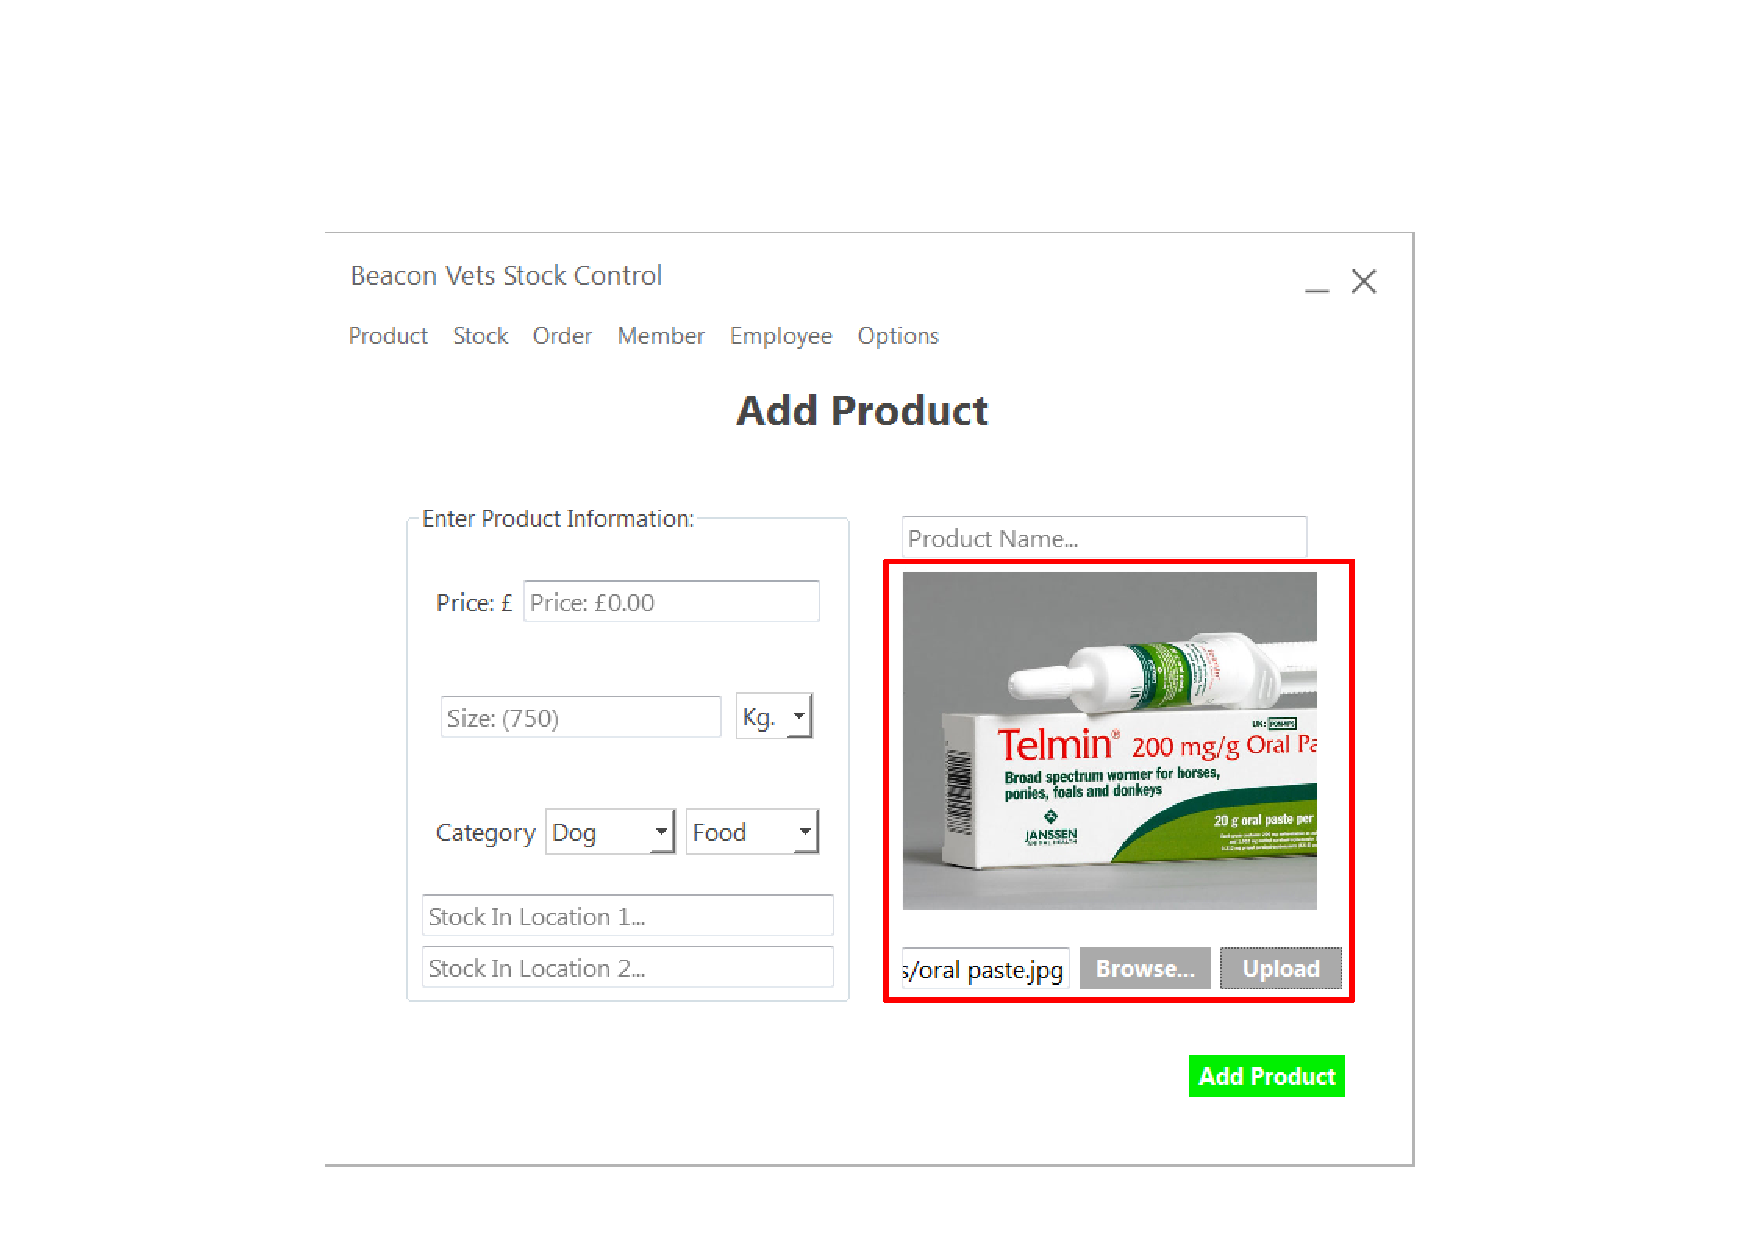
\includegraphics[width = \textwidth]{./Evaluationimages/learnability-1.pdf}

If someone is not obvious to the user, i tried to add a label that tells the user what to do. An example of this, can be found on the preferences interface.
In the screenshot below i used a QLabelt hat will display a message to the user when it is clicked. In this example, the system tells the user what the email address and password are used for.

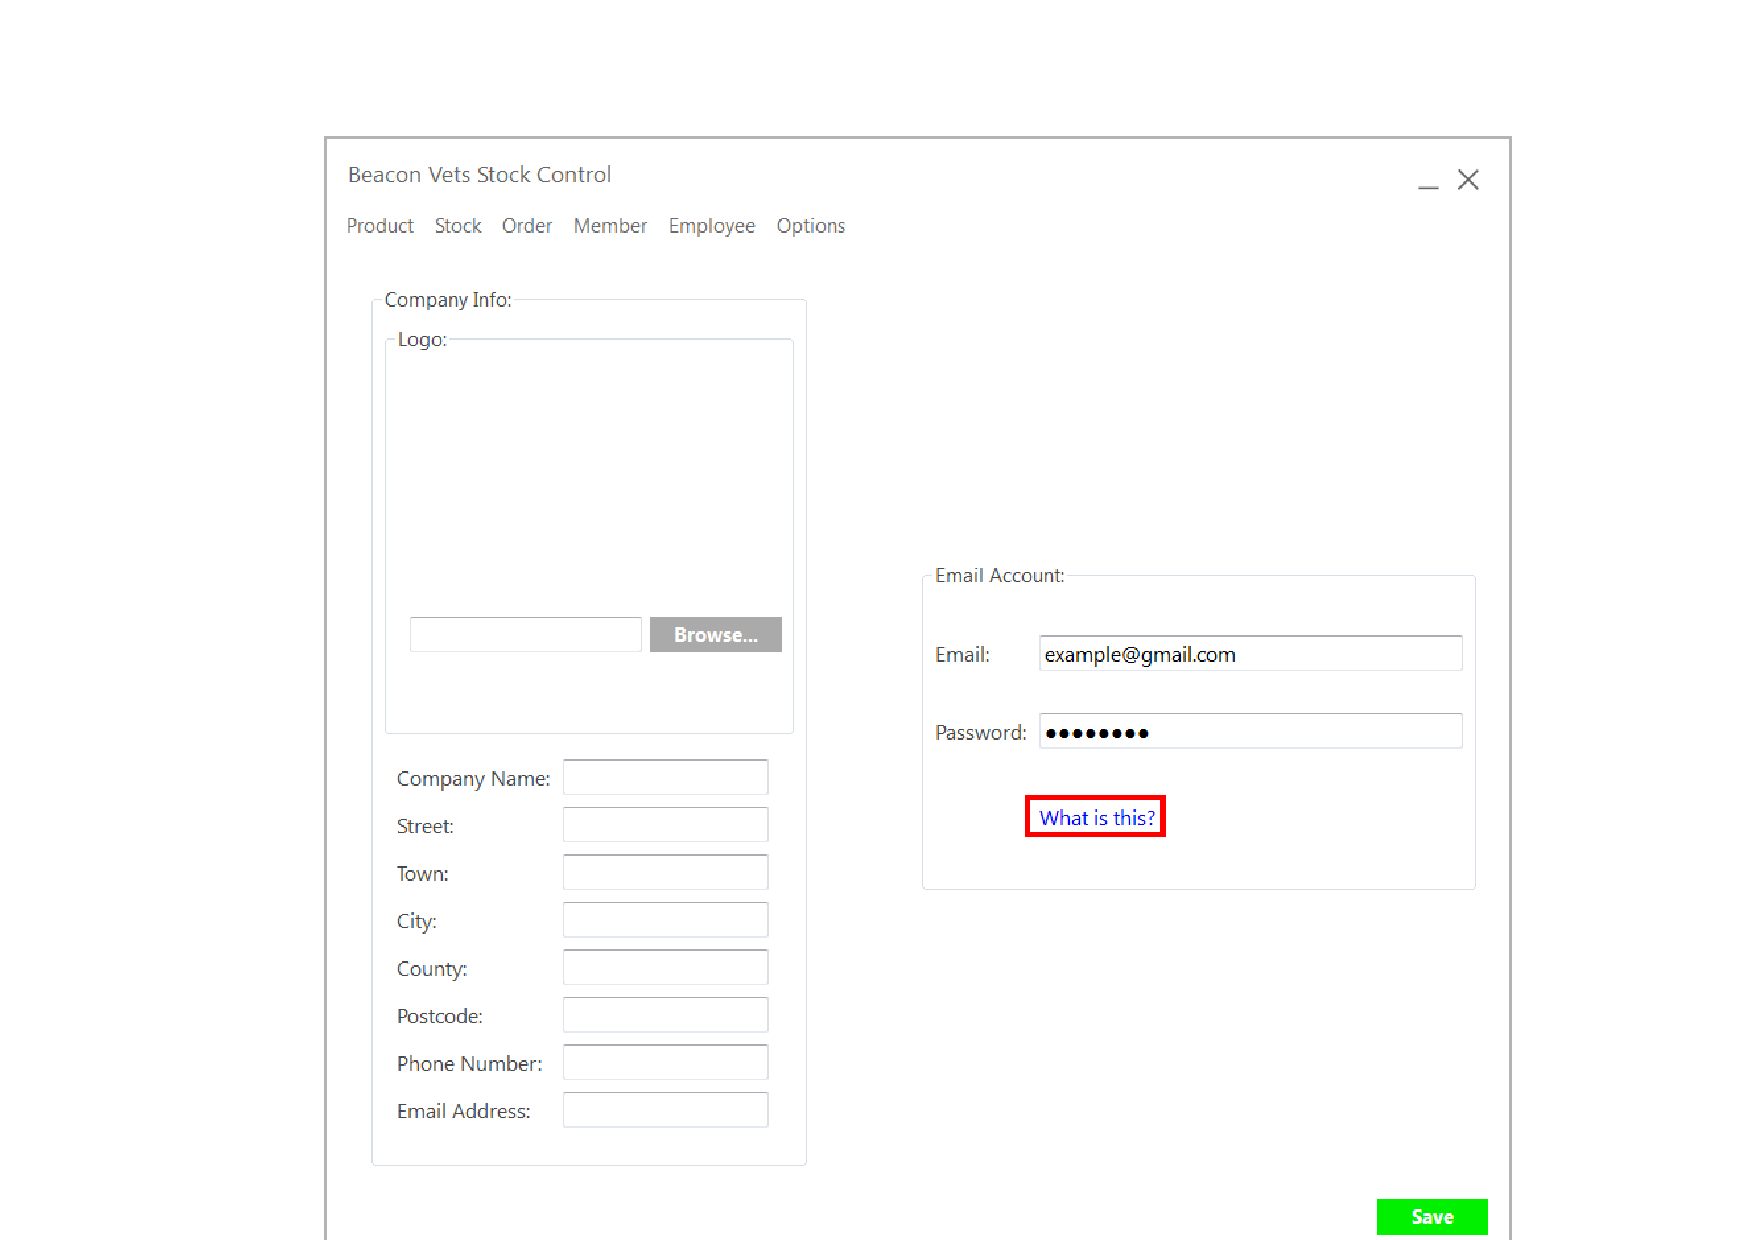
\includegraphics[width = \textwidth]{./Evaluationimages/learnability-2.pdf}

When deciding on the keyboard shortcuts, i tried to use shortcuts that may have a similar meaning in other programs in which the users have used. In a lot of word processors, the keyboard shortcut `CTRL+F' is usually used to find something in the document. My clients current system is done on Microsoft excel, which also uses this keyboard shortcut for searching for data within the spreadsheet. I felt this could be related to my system to access the search window, when the user wants to find something within my system. Therefore, i decided to assign the keyboard shortcut `CTRL+F' to access the search window.


\pagebreak
\section{Usability}

I designed my system to have the highest usability possible. The main points to consider when increasing the usability of a system are listed below.

\begin{itemize}
	\item{Target Acquisition Time}
	\item{Latency}
	\item{Readability}
	\item{Use of metaphors}
	\item{Navigability} 
\end{itemize}

\subsection{Target Acquisition Time}

When designing my system, i wanted to make use of Fitt's Law to increase the usability of my system. Fitt's law states that: ID=log2(2A/W) where ID is the index of difficulty, A is the distance to move and W is the size of the target.

Looking at the `Add Product' interface below, i feel i could have improved the target acquisition time of the interface.

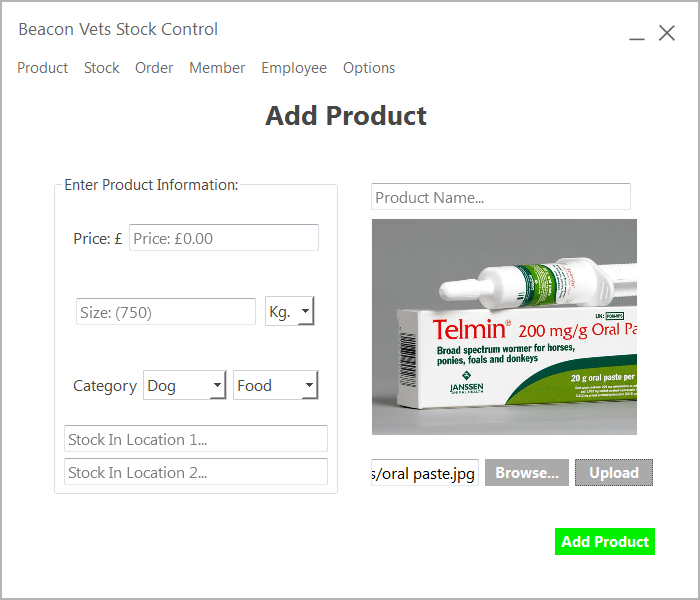
\includegraphics[width = \textwidth]{./Evaluationimages/learnability-1.png}

There is a large vertical space above and below the title of the interface. This will increase the distance the user has to move the mouse when wanting to access the Menubar. All the data fields within the `Enter Product information' have been grouped together as close as possible to reduce the index of difficulty as much as possible, to reduce the time it takes to enter the data into the data fields. The Add Product button is quite far away from the rest of the widgets within the interface and the index of difficulty could be reduced by reducing the spacing between the button and the other widgets.

Trying to maintain a low index of difficulty was hard for the creating order interface is it had to include a lot of different widgets. Below is a screenshot of the
creating order interface.

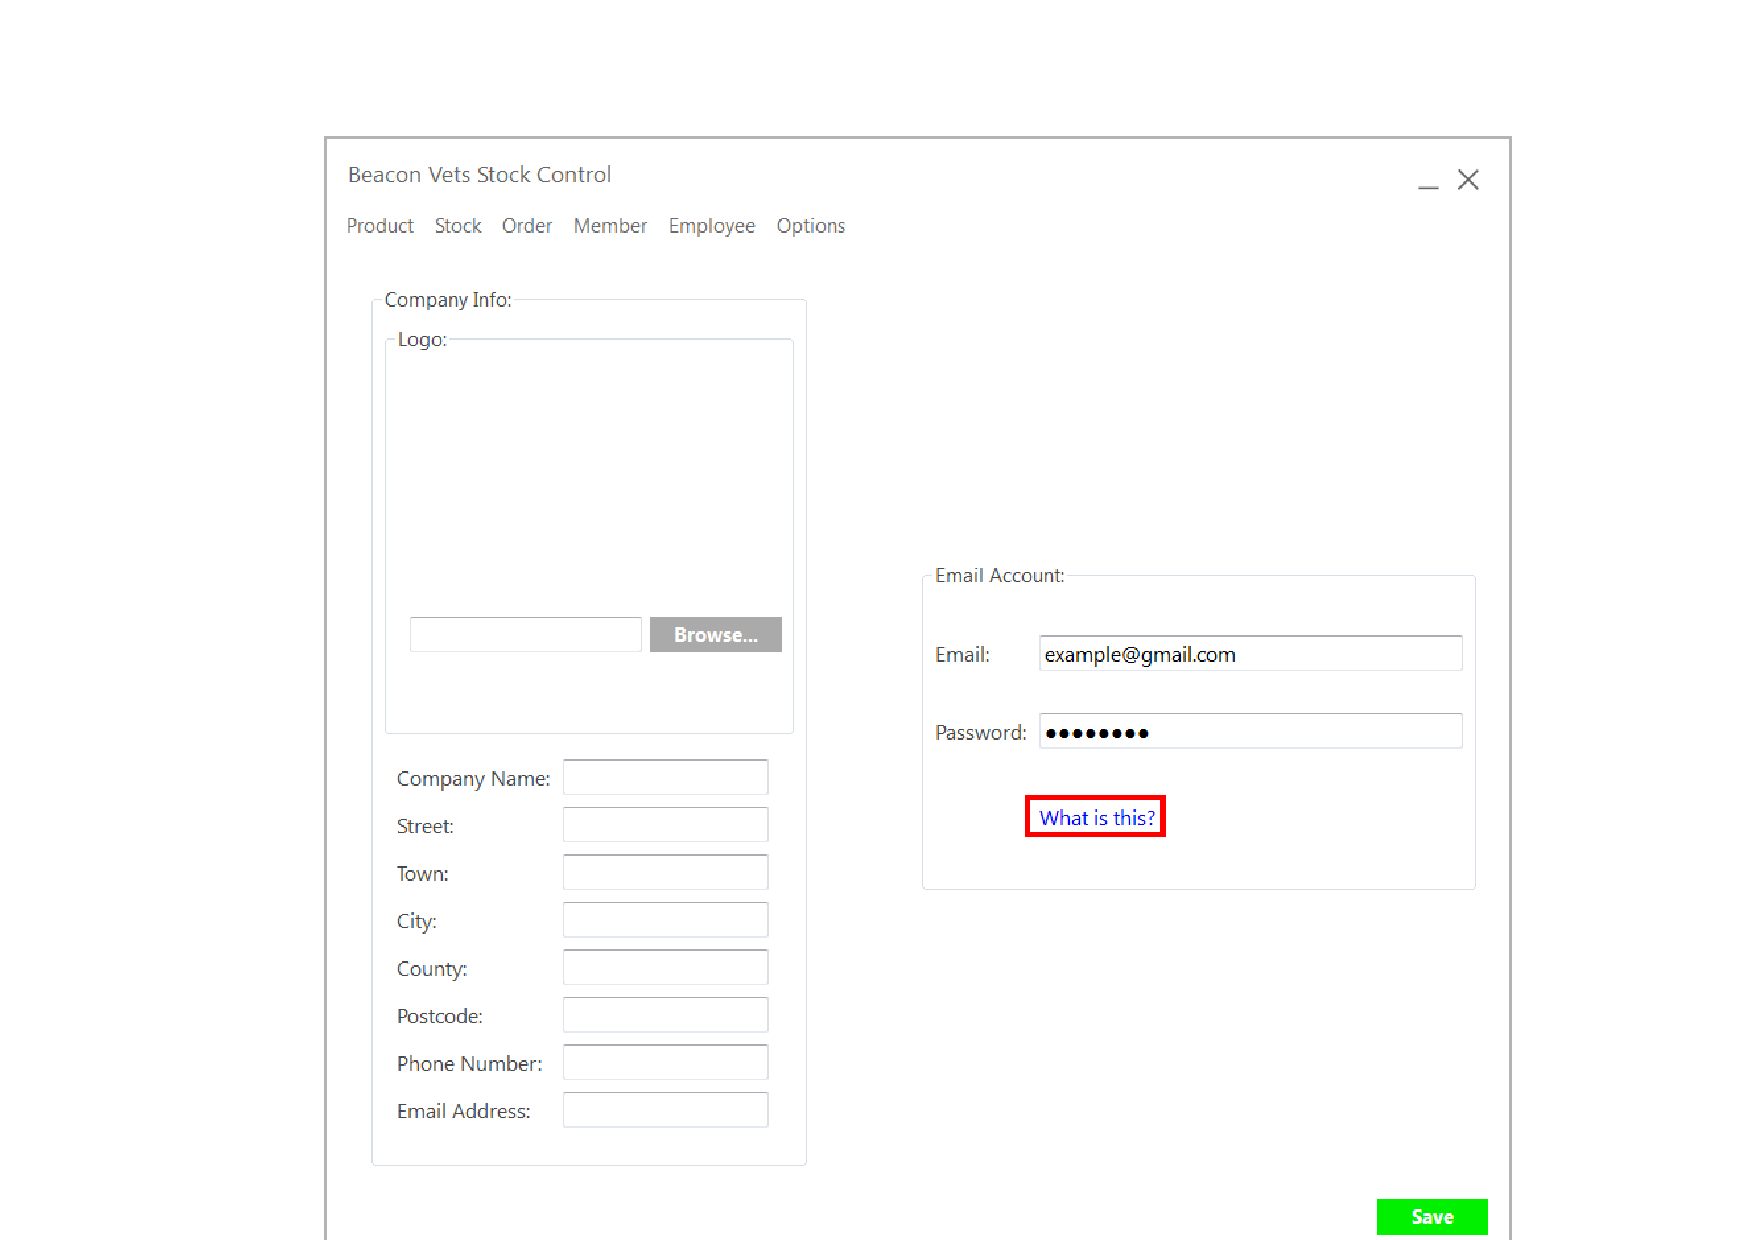
\includegraphics[width = \textwidth]{./Evaluationimages/learnability-2.png}

Because the creating order interface requires far more widgets than the other interfaces, i had to increase the size of the window compared to the other interfaces. I tried to make the size of the interface as small as possible without the widgets being too bunched together. I felt that the user would want to preview the invoices regularly so i made this button larger than the add to order button because i feel this button is less important because most users can double click on the product to add it to the order. Increasing the size of the button will decrease the difficulty index due to Fitt's Law.

In general, I increased the size of all the QPushButtons within the system to decrease the overall difficulty index. Aswell as having issues when the system is scaled, i decided to fix the size of the window because as the size of the window, the more my widgets would spread out, increasing the difficulty index.

\subsection{Latency}

All of the button clicks within my system take less than 50 milliseconds apart from one button. When the user wants to change their password, an email is sent to their account with a code which takes just over a second to send and change interface. An improvement to the system could be to change the cursor to an animated hour glass when this button is clicked to tell the user the system is still functioning correctly.

Before i removed the functionality of displaying an image in the search window. The process of displaying the images took roughly 10-15 seconds. Here i could have used a progress indicator so the user can see how far through the process the system is, and also include an audible sound when the system has completed the process. However, whenever the system tried to load the images they system became unresponsive so the user would not be able to see the progress bar.

\subsection{Readability}

The readability of the all QLabels and QLineEdits is very good as it is very dark grey text on a white background. I felt that black text on a white background contrasted too much so i decided to make the text a very very dark grey. I wanted to important buttons bright green so they are noticed by the user easily. However the dark grey text and light green button contrasted too much so i decided to make the text in the green buttons white. this made the text contrast much less and made it far more readable. I increased the size of the text and changed the font to, in my opinion, a font that is easier to read. I also decided to have alternating row colours in the tables to make data easier to read from the table.


\subsection{Use of metaphors}

Within my system i did not use any metaphors. All the other data fields are described using a QLabel with text to describe what to enter. Some examples of metaphors that could be used within my system are a magnifying glass could be used to represent the Search Window. The icon could be displayed in the Options menu in the drop down menu. Adding a product could be represented with the `+' symbol and deleting a product could be represented by the `x' symbol. 

\subsection{Navigability} 

The user can navigate the system easily using the Menubar at the top of the system. The menubar is displayed whenever the user is currently logged into the system, it is shown in the screenshot below of the creating order interface.

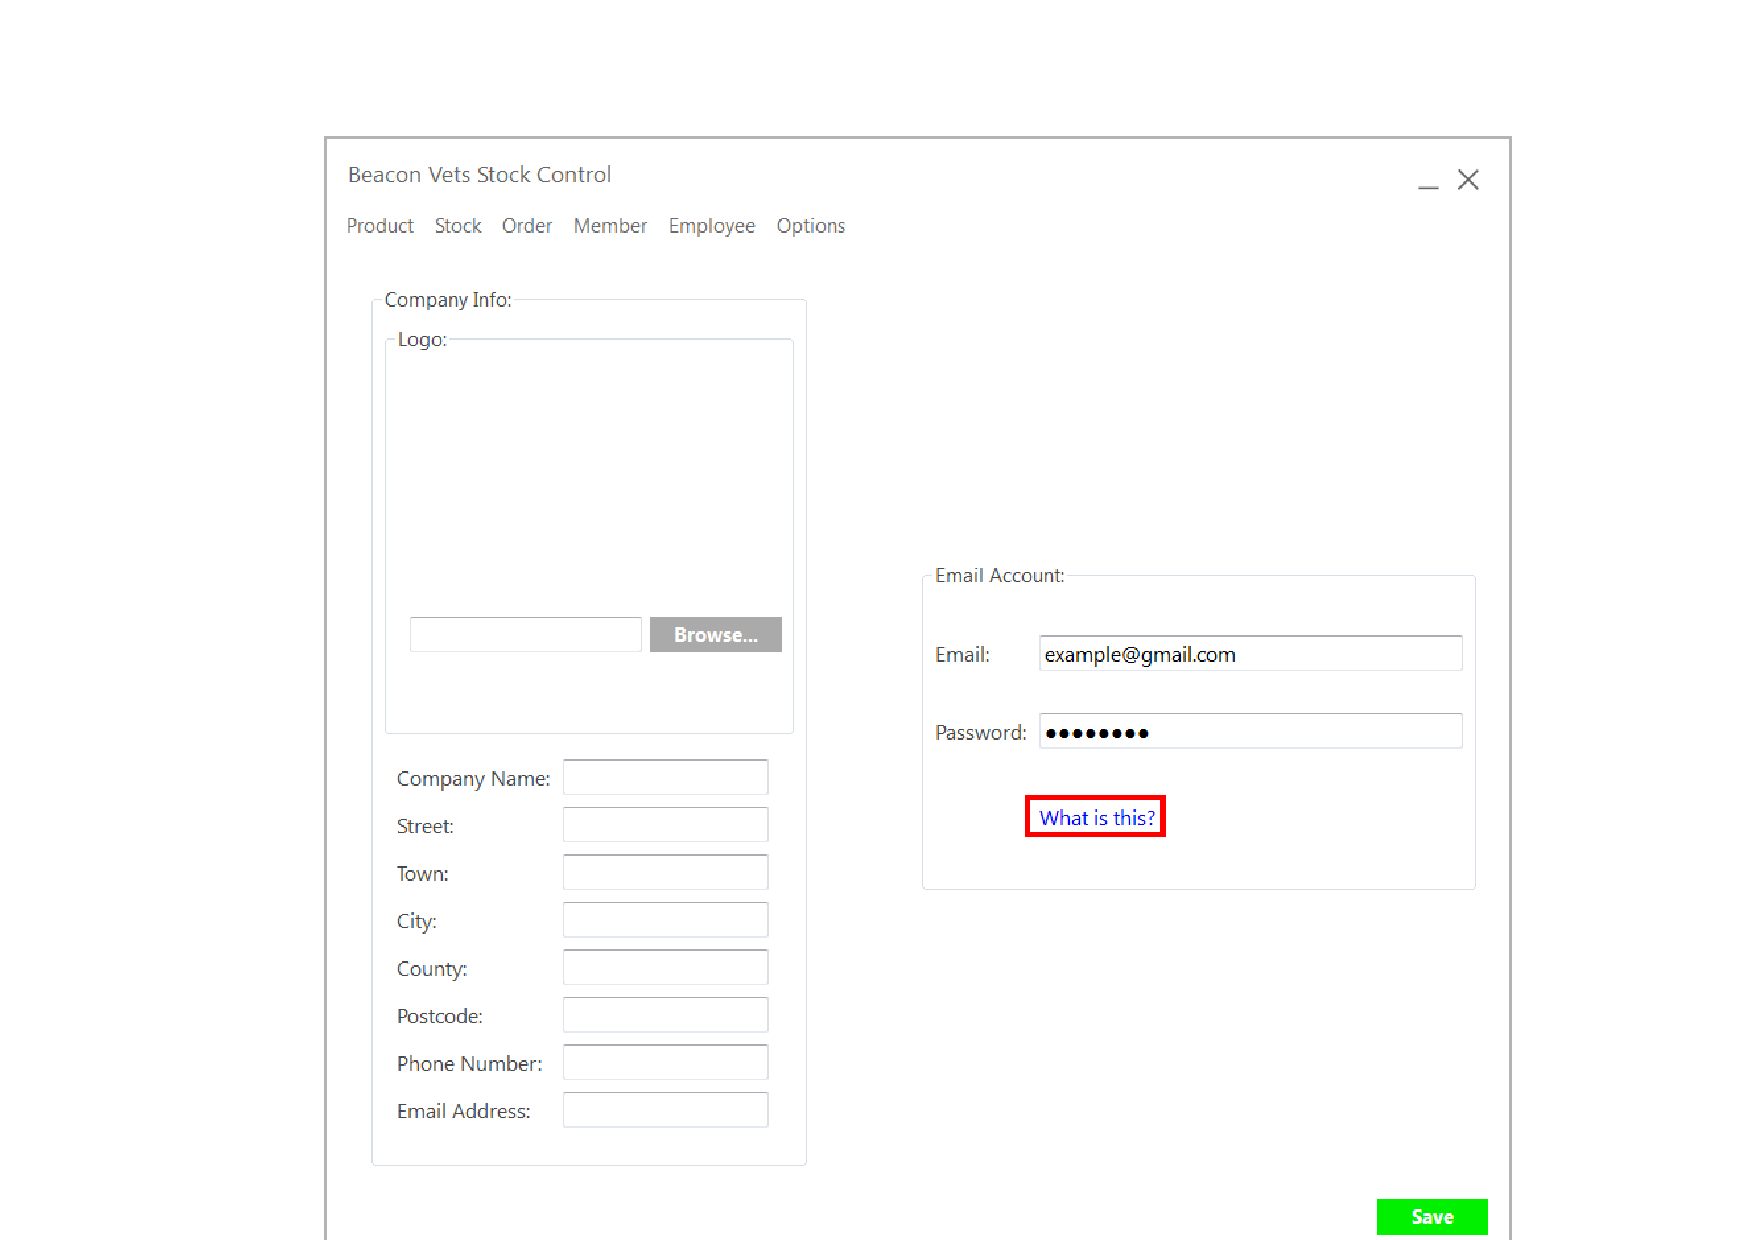
\includegraphics[width = \textwidth]{./Evaluationimages/learnability-2.png}

Before the user logs into the system, the user cannot access the Menubar. This is to prevent the user from being able the user to access the system before they log in. Below the log in interface is shown.

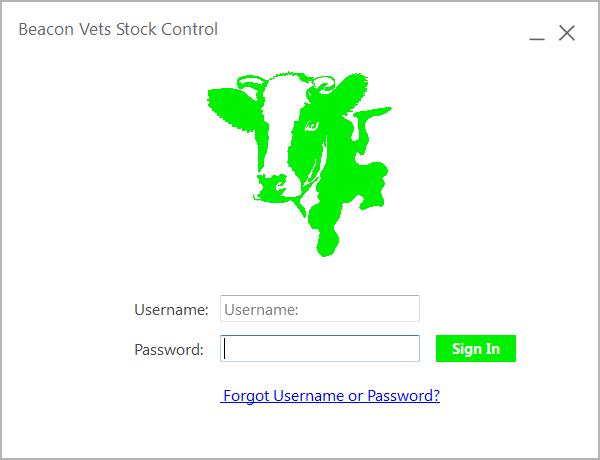
\includegraphics[width = \textwidth]{./Evaluationimages/learnability-3.png}

If the user clicks on the `Forgot Username and Password' label, the user is taken to another interface. This interface has a button that allows the user to return to the log in interface if they accidentally clicked on the button.This is shown in the screenshot below.

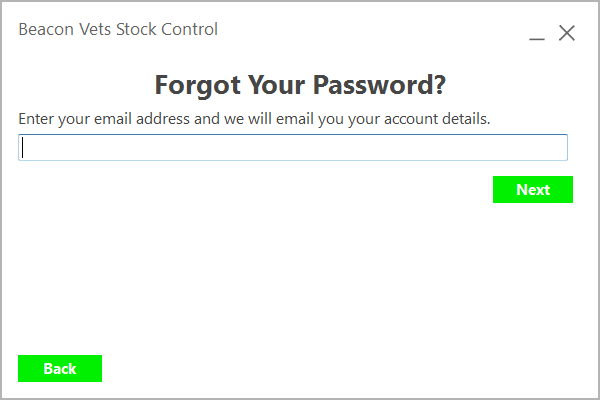
\includegraphics[width = \textwidth]{./Evaluationimages/learnability-4.png}

Currently, the system has now ay to undo the changes made once they have been made. However before adding, editing or deleting a product member or employee the user is presented with a confirmation window to ensure they want to add edit or delete the product member or employee. This reduces the chance of changes being made accident by accidentally clicking buttons. If the user accidentally clicks the add product button, they can simply click `No', when asked if they're sure they want to add the product.

\pagebreak
\section{Maintainability}

\subsection{Changing Parameters}

In the current system, all members get 10\% off. My client may want to increase or decrease this discount in the future, which means i would have to change the current discount rate which is currently 0.1 (10\%). In a future version of the system, i could add this as a preference under the preferences menu where the user could tell the system the percentage the discount should be.

When the stock of a product falls below 5, the system tells the user that the product needs to be restocked. Some products may sell in large quantities, in which case the user might want to be warned when stock falls below 50/40 for example. This could be modified in a future version of the system, so that another column is added to the Product table, storing the value in which the user should be warned if the stock falls below. this value could then be changed by the user in the manage stock interface.

When the system is first run, an admin account is first created with the first name Tom, last name Henderson and username Thenderson1. This is the name of my client, who will be the administrator of the system. This account cannot be edited in the system. If i were to distribute the system to a different client, the first name, last name and username would have to be changed accordingly. This could be resolved in a future version of the system where the user must enter their first name and last name upon the first start up, which will then be used to create the admin account.

\subsection{Responding to new Requirements.}

In the future, when the company starts to sell more and more products, trying to find a product in the system may take a long time. Integrating the use of a bar code scanner will mean the user does not have to find a product in the system and the product can automatically be added to the order. this will rapidly decrease the time it takes to create an order.

The company may also want to sell a different type of product that may need to store data. For example the veterinary centre could sell medication, which may need to store the size of each dose, the time between each dose application ect. This would require me to create a new data field to store the dose size and time between each application.

If the company changes their logo, i have given the user the option to be able to change it on the invoice that is sent out to the customer, however, the logo used on the log in screen has been hard coded. A small change could be made so that the logo used on the invoice is also used on the log in screen, so that the system can be used for other clients.

\pagebreak
\section{Suggestions for Improvement}

From the feedback from question 14 of the questionnaire, several users suggested that the user should be able to change the colour scheme of the system as they felt some of the green buttons were too bright. A future version of the system could include a new option in the preferences interface where the user can select the colour scheme of the system. 

Another suggestion from the user feedback from question 10 of the questionnaire was that more keyboard shortcuts should be implemented. The users that made use of the keyboard shortcuts could then navigate the system faster, which is the main concept of the keyboard shortcuts. The problem that could be encountered implementing new keyboard shortcuts is that, it may become hard to remember all of the shortcuts and their functions, especially for new users to the system.

Implementing more keyboard shortcuts would also mean the shortcuts would have less meaningful shortcuts as the meaningful ones have already been used. This would also increase the learning curve for users with little computer knowledge.

An improvement suggested by a user from the feedback in the questionnaire, is that the system should display the recent sales of each product. Currently the graph only displays the sales of previous weeks and day not the current week or day. This could easily be implemented intot he system as the current weekly and daily sales are already being recorded by the system, however, they are not displayed tot he user.

\pagebreak
\section{End User Evidence}

\pagebreak
\subsection{Questionnaires}

The questionnaire given to my client differed slightly to the questionnaire given tot he other users. I had more time to discuss the problems with the system, with my client compared to the other users of the system, which i did not have time to discuss the problems. Therefore, the questionaire given to my client, contains more detail, and gives a better evaluation of the system objectives compared to the other users.

\subsubsection{Questionnaire 1 (Client)}

\label{Client-Q1}
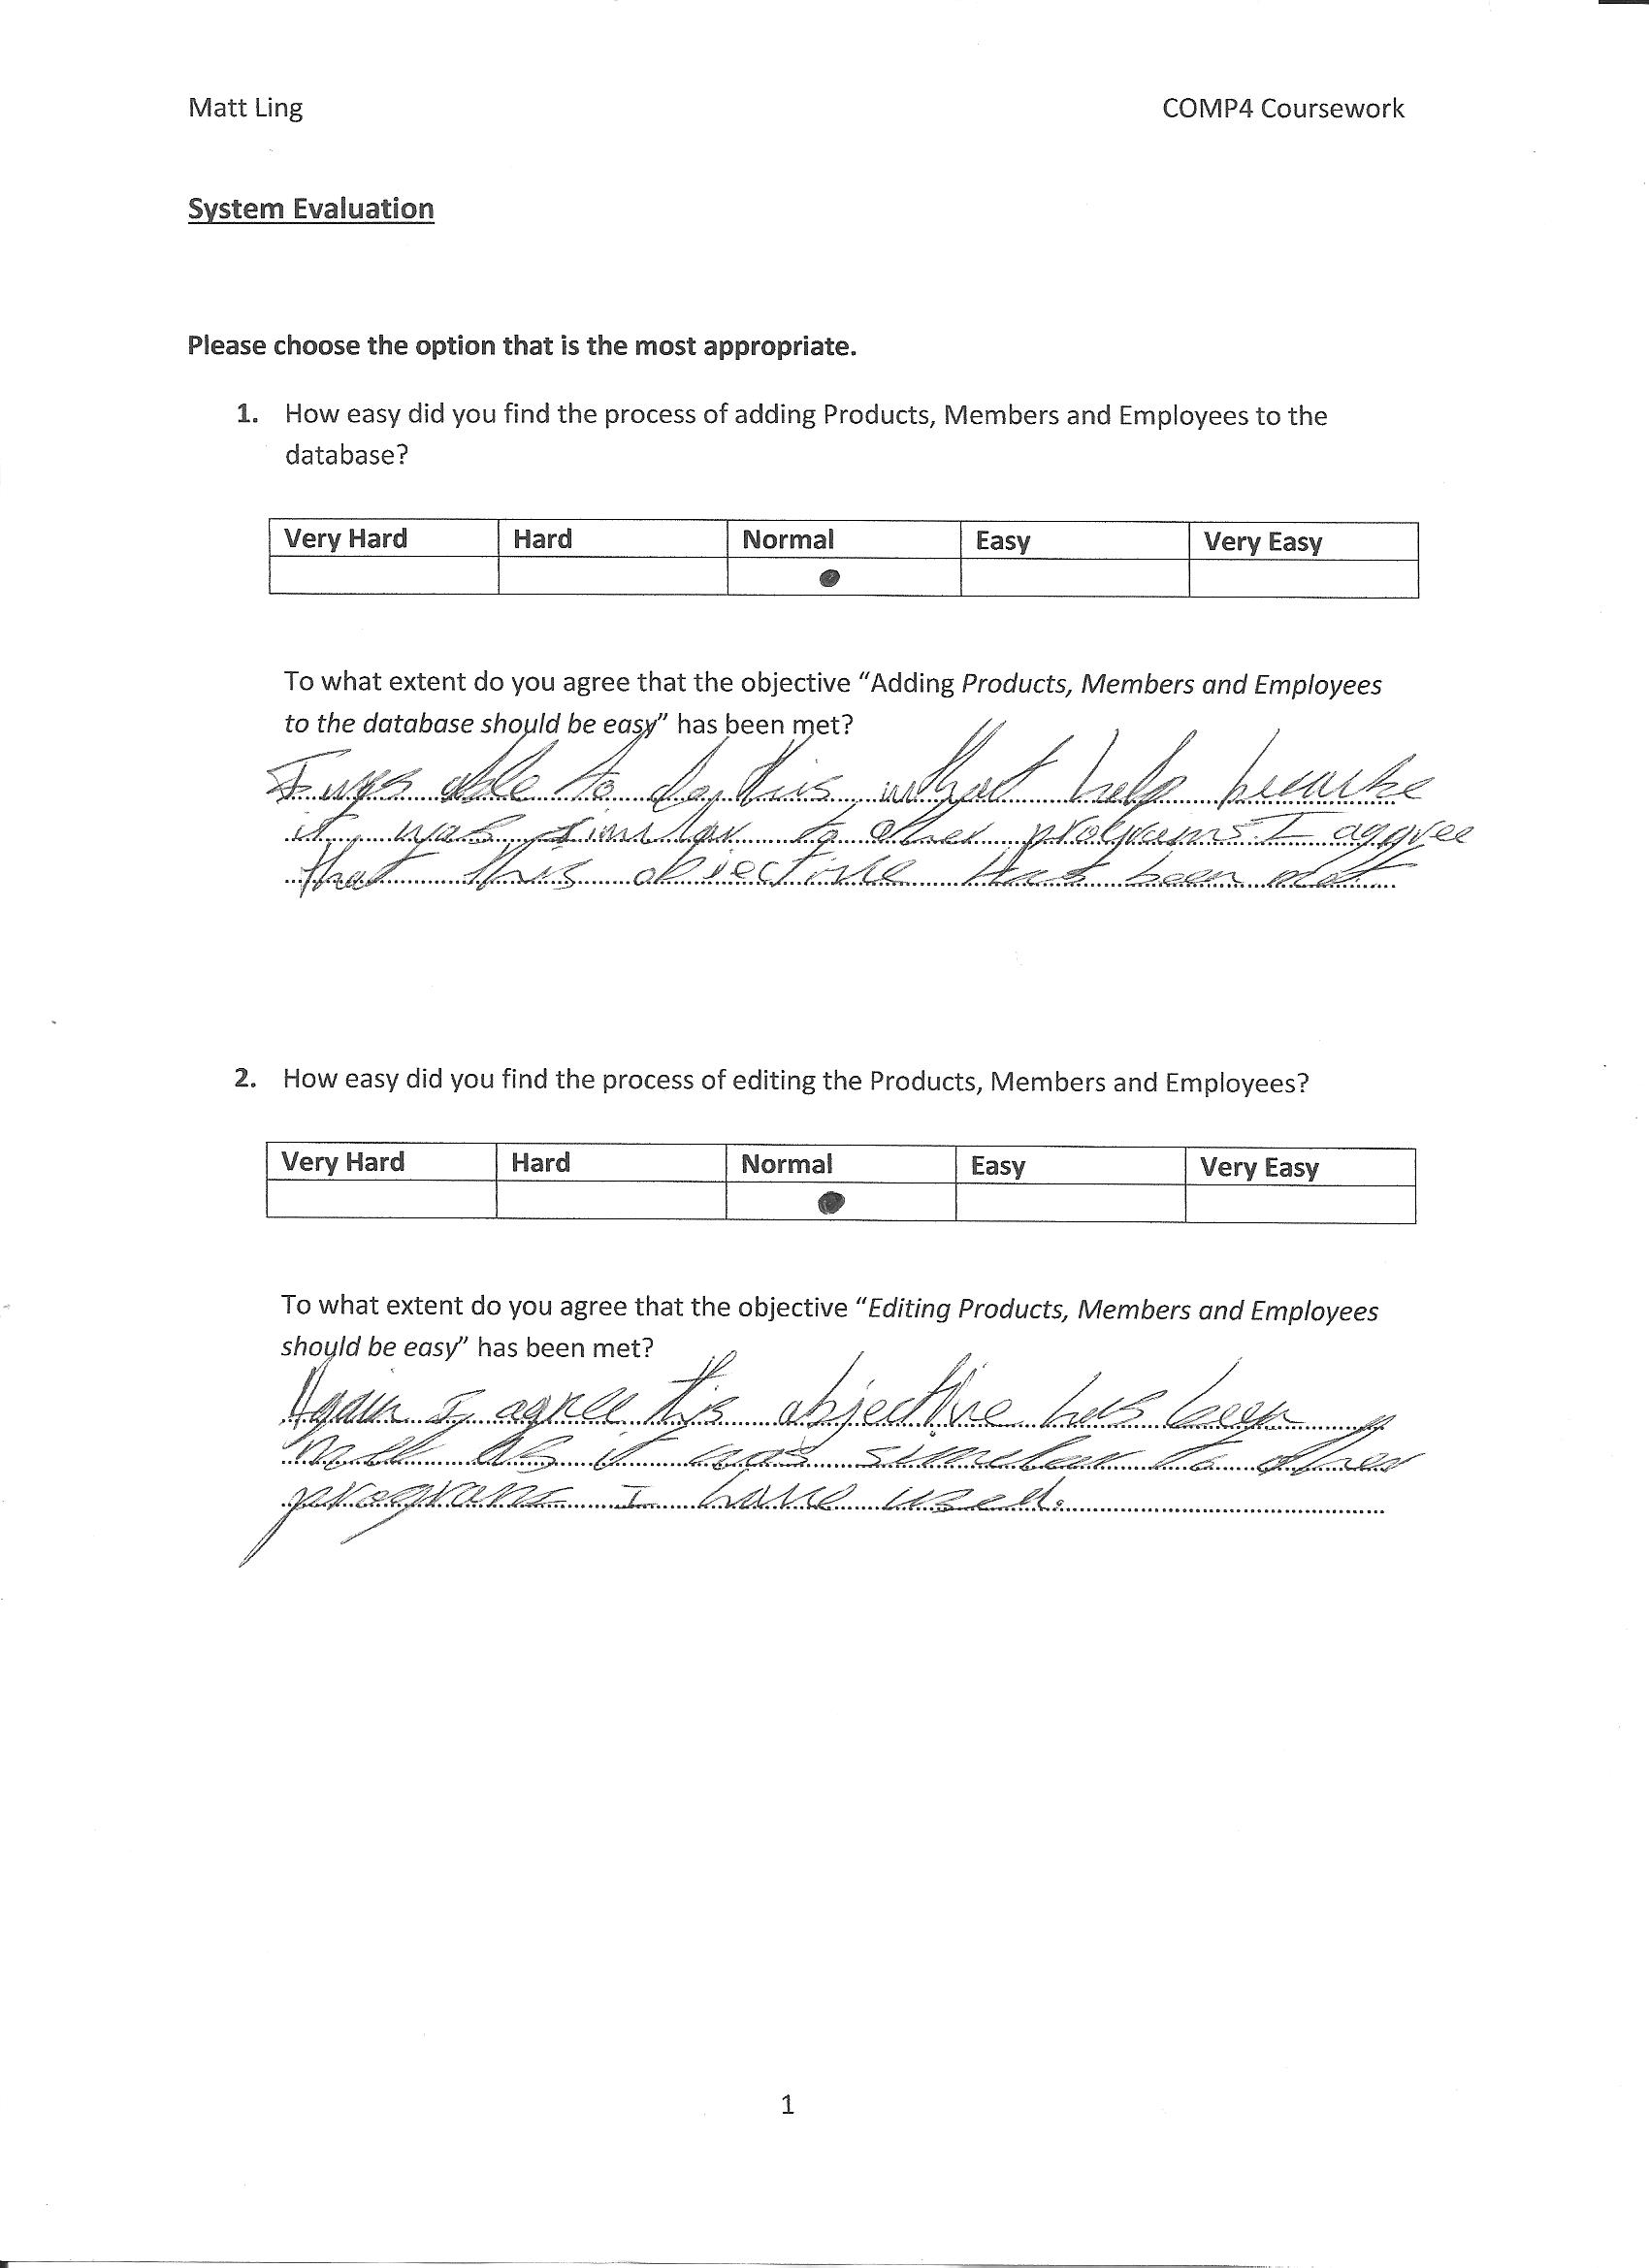
\includepdf{./EvaluationImages/tom-1.jpeg}
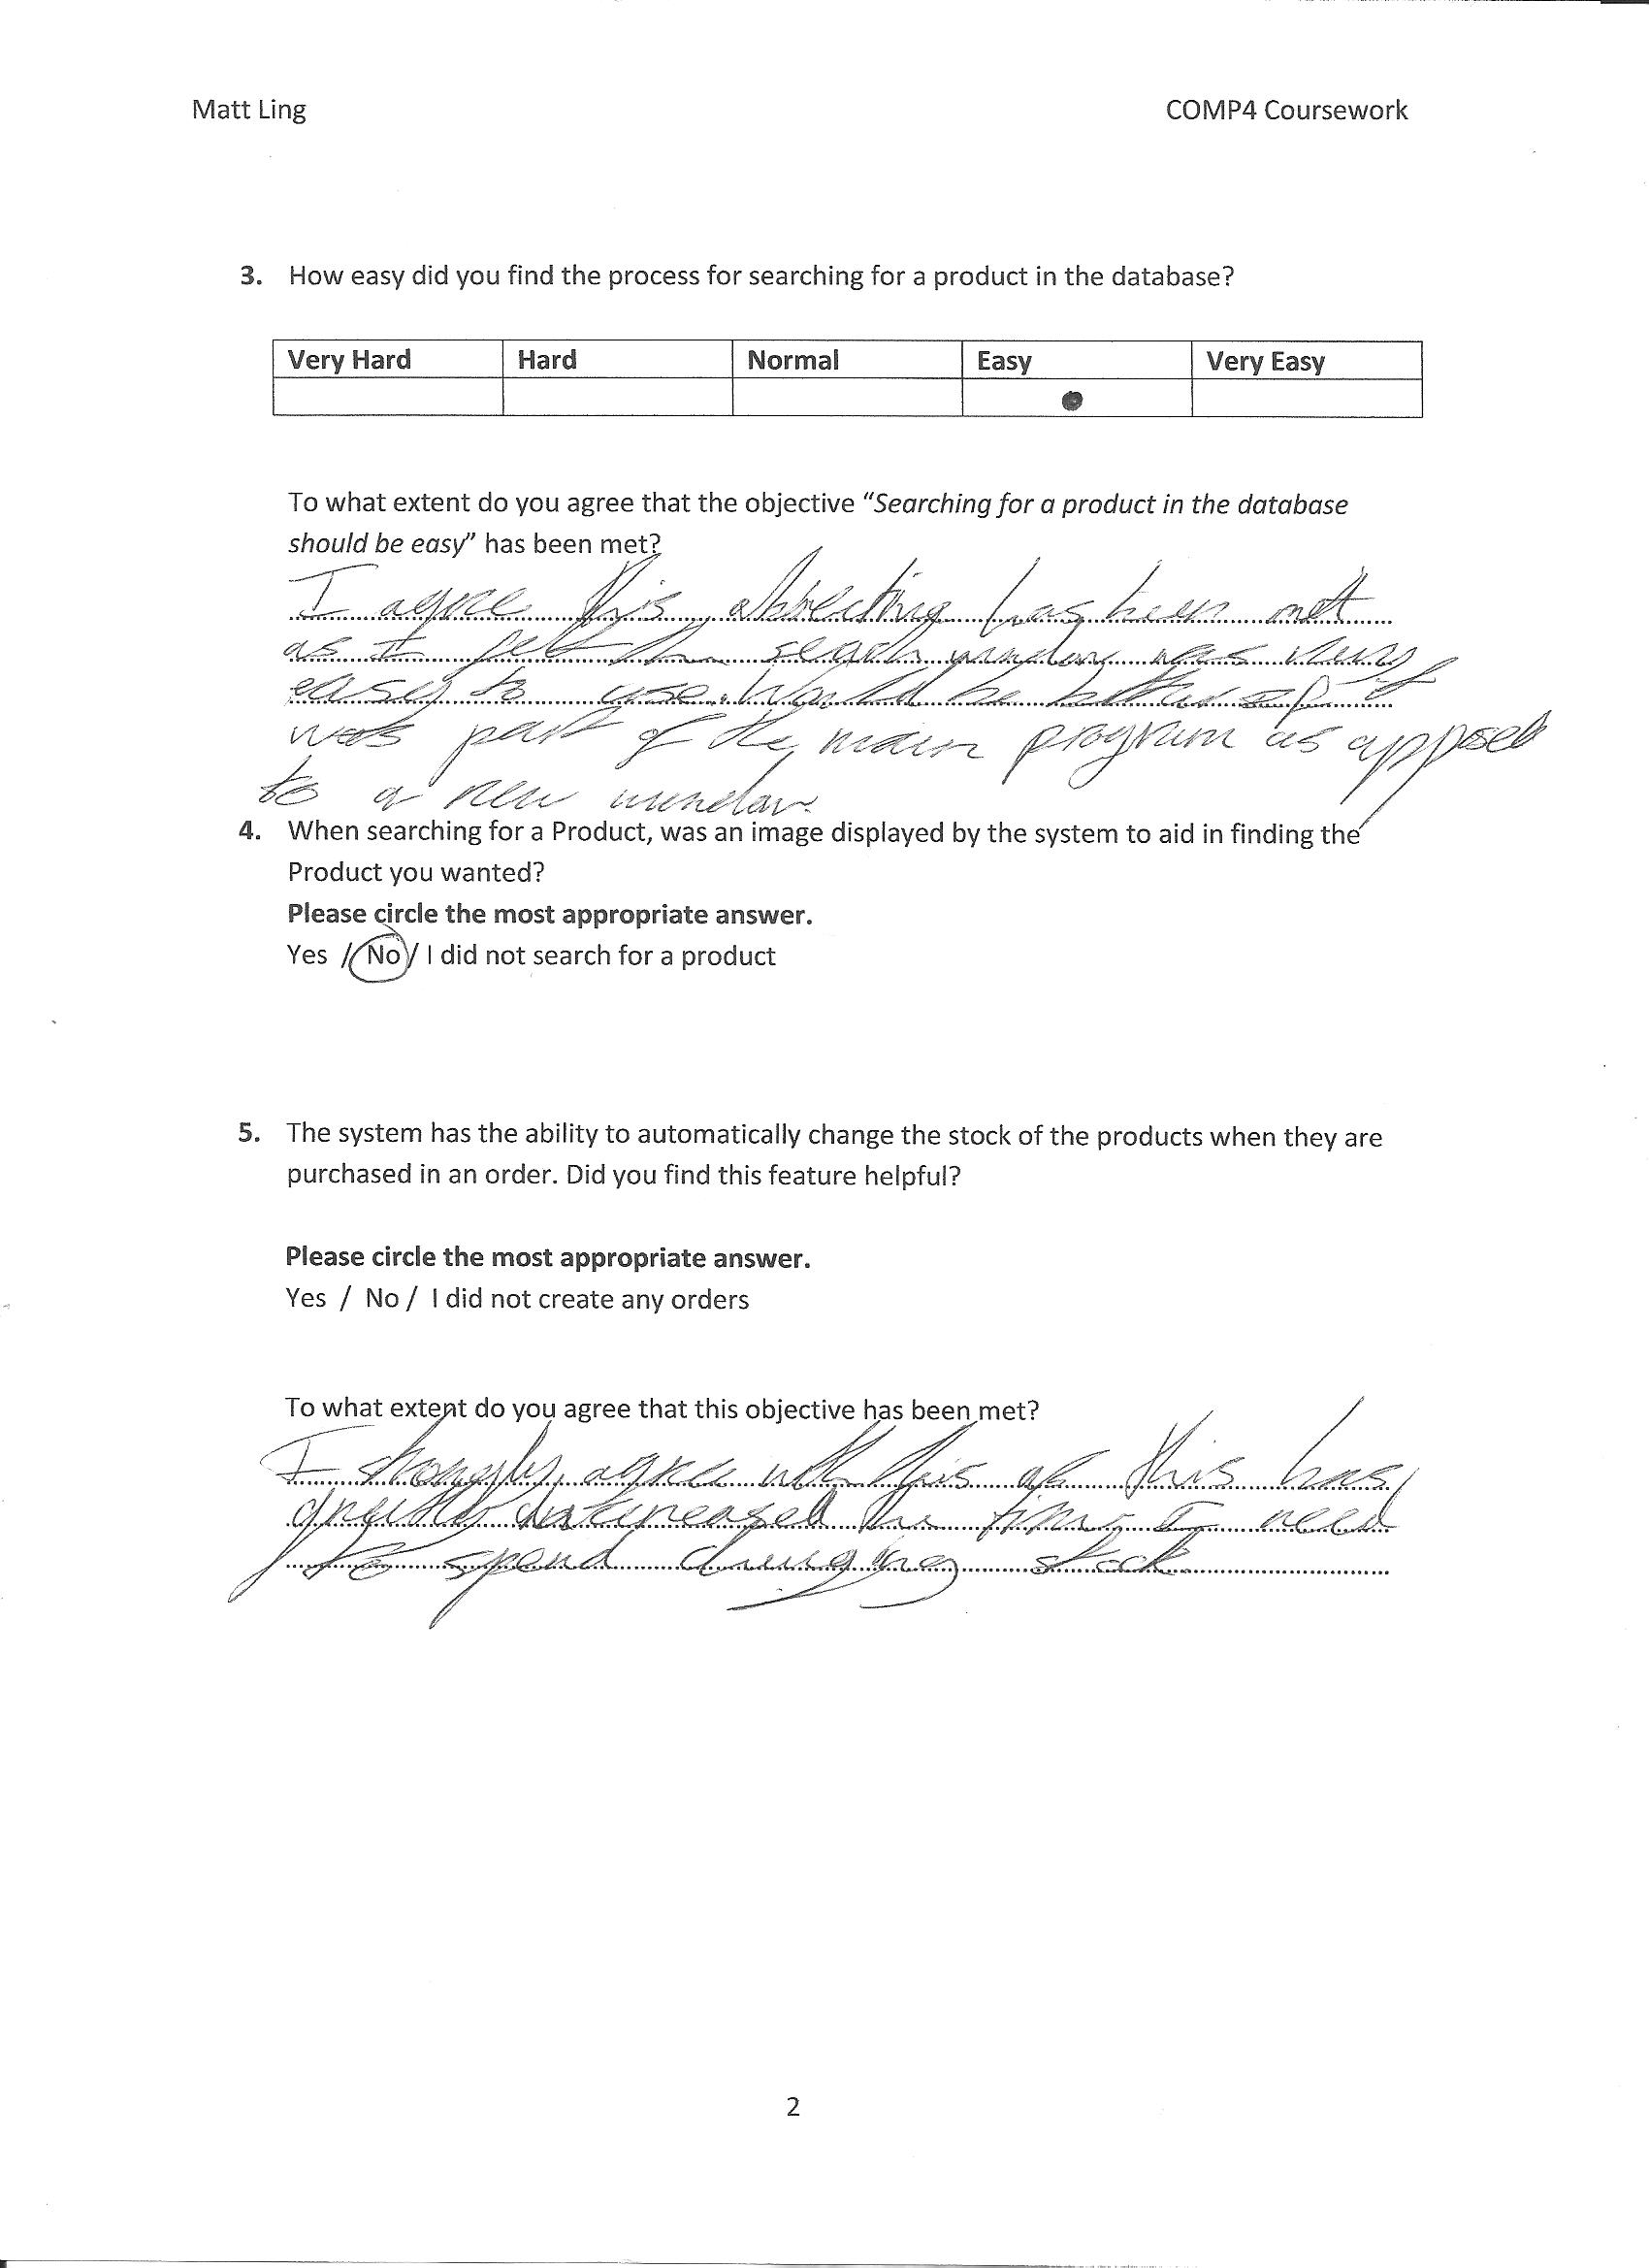
\includepdf{./EvaluationImages/tom-2.jpeg}
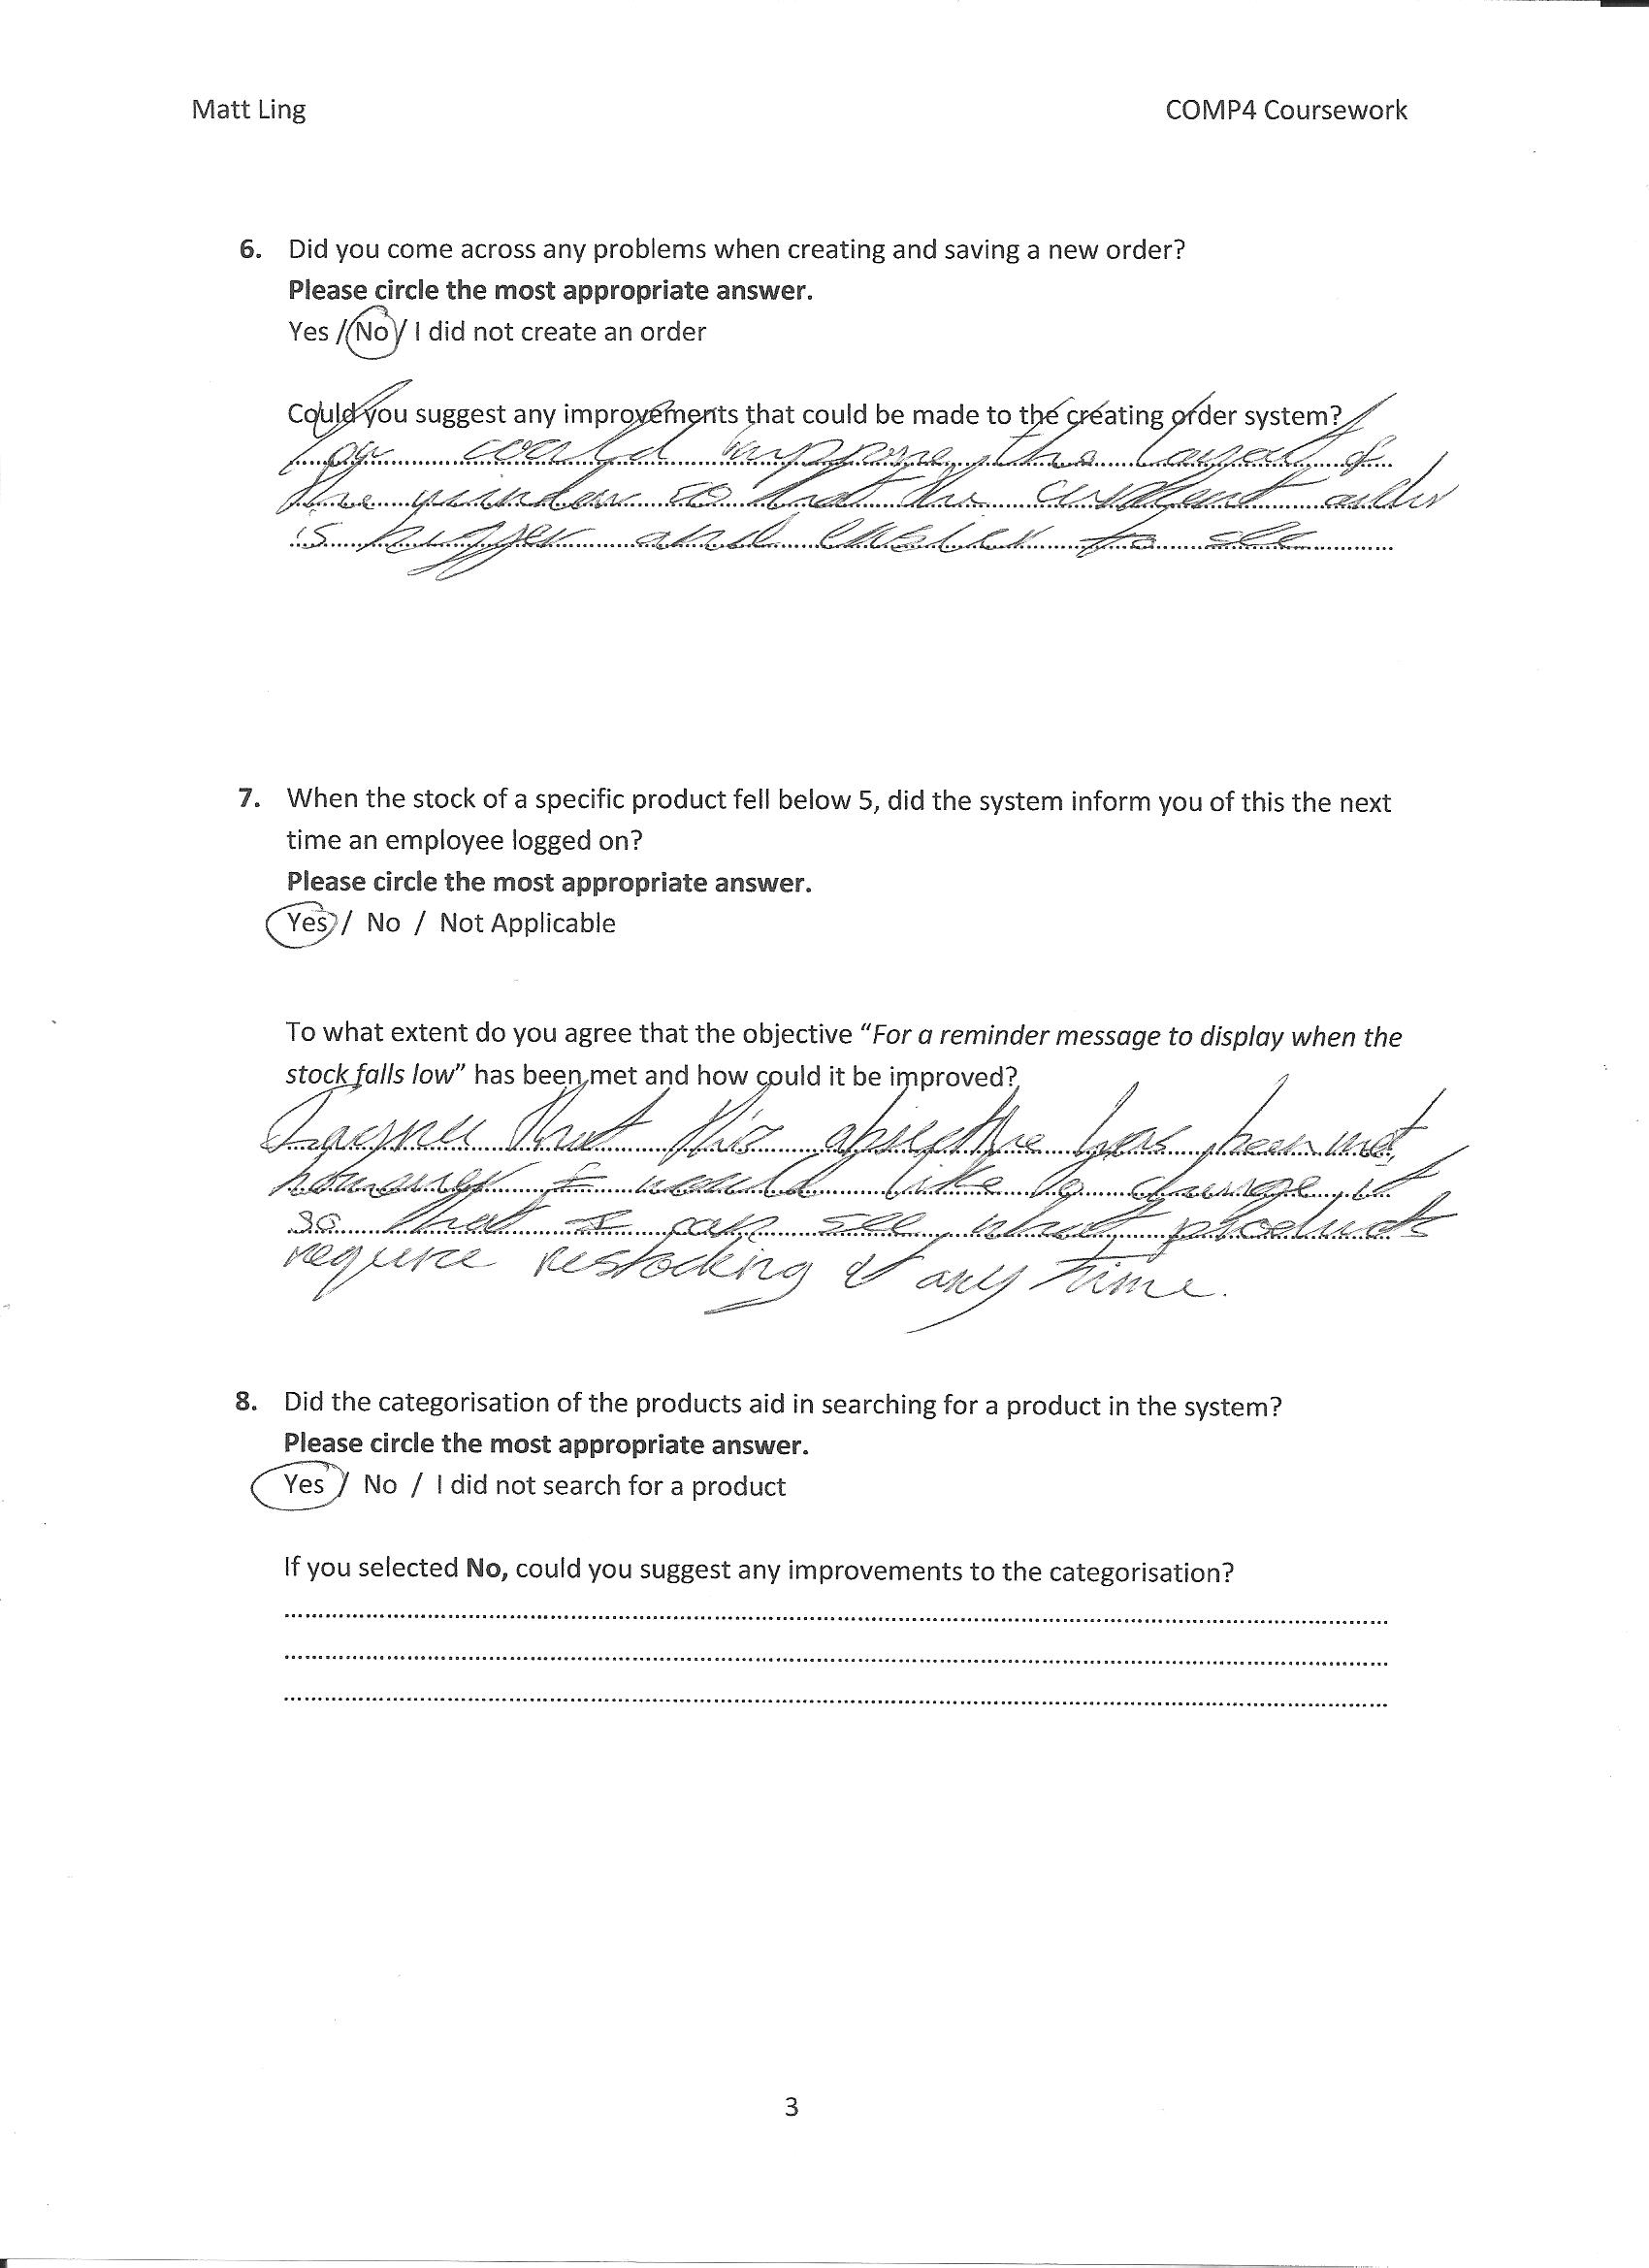
\includepdf{./EvaluationImages/tom-3.jpeg}
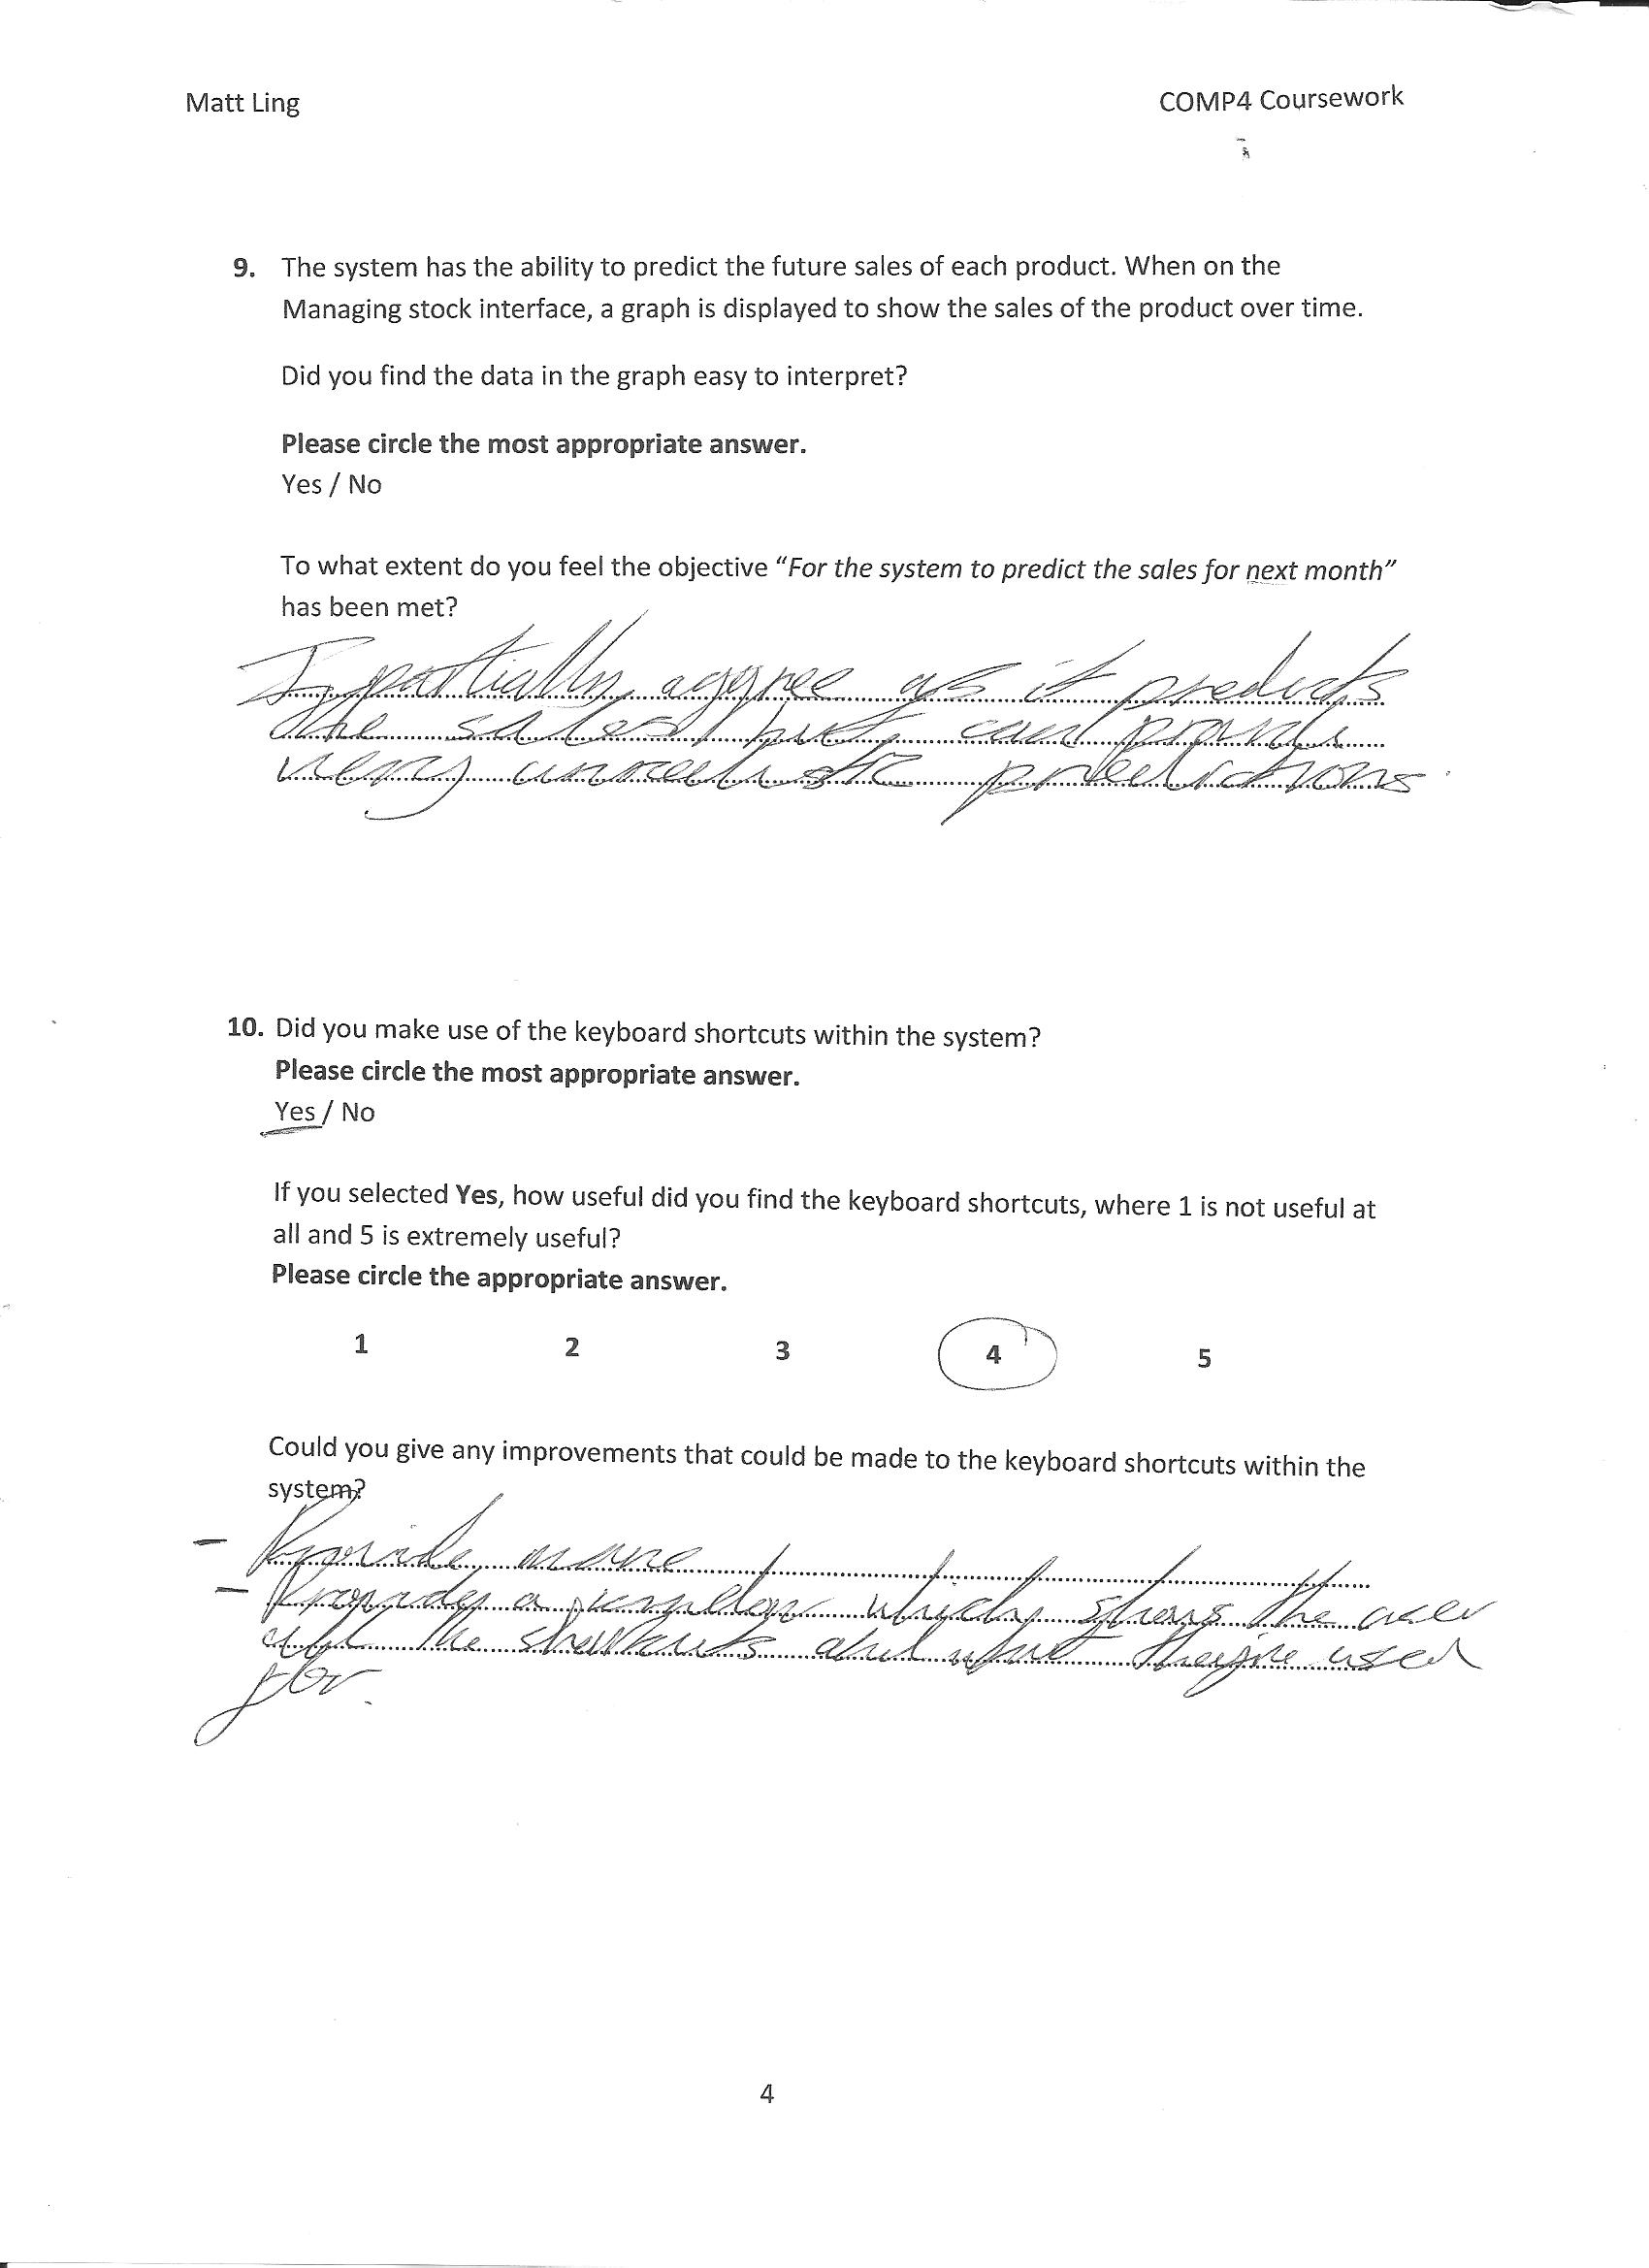
\includepdf{./EvaluationImages/tom-4.jpeg}
\label{Client-Q11}
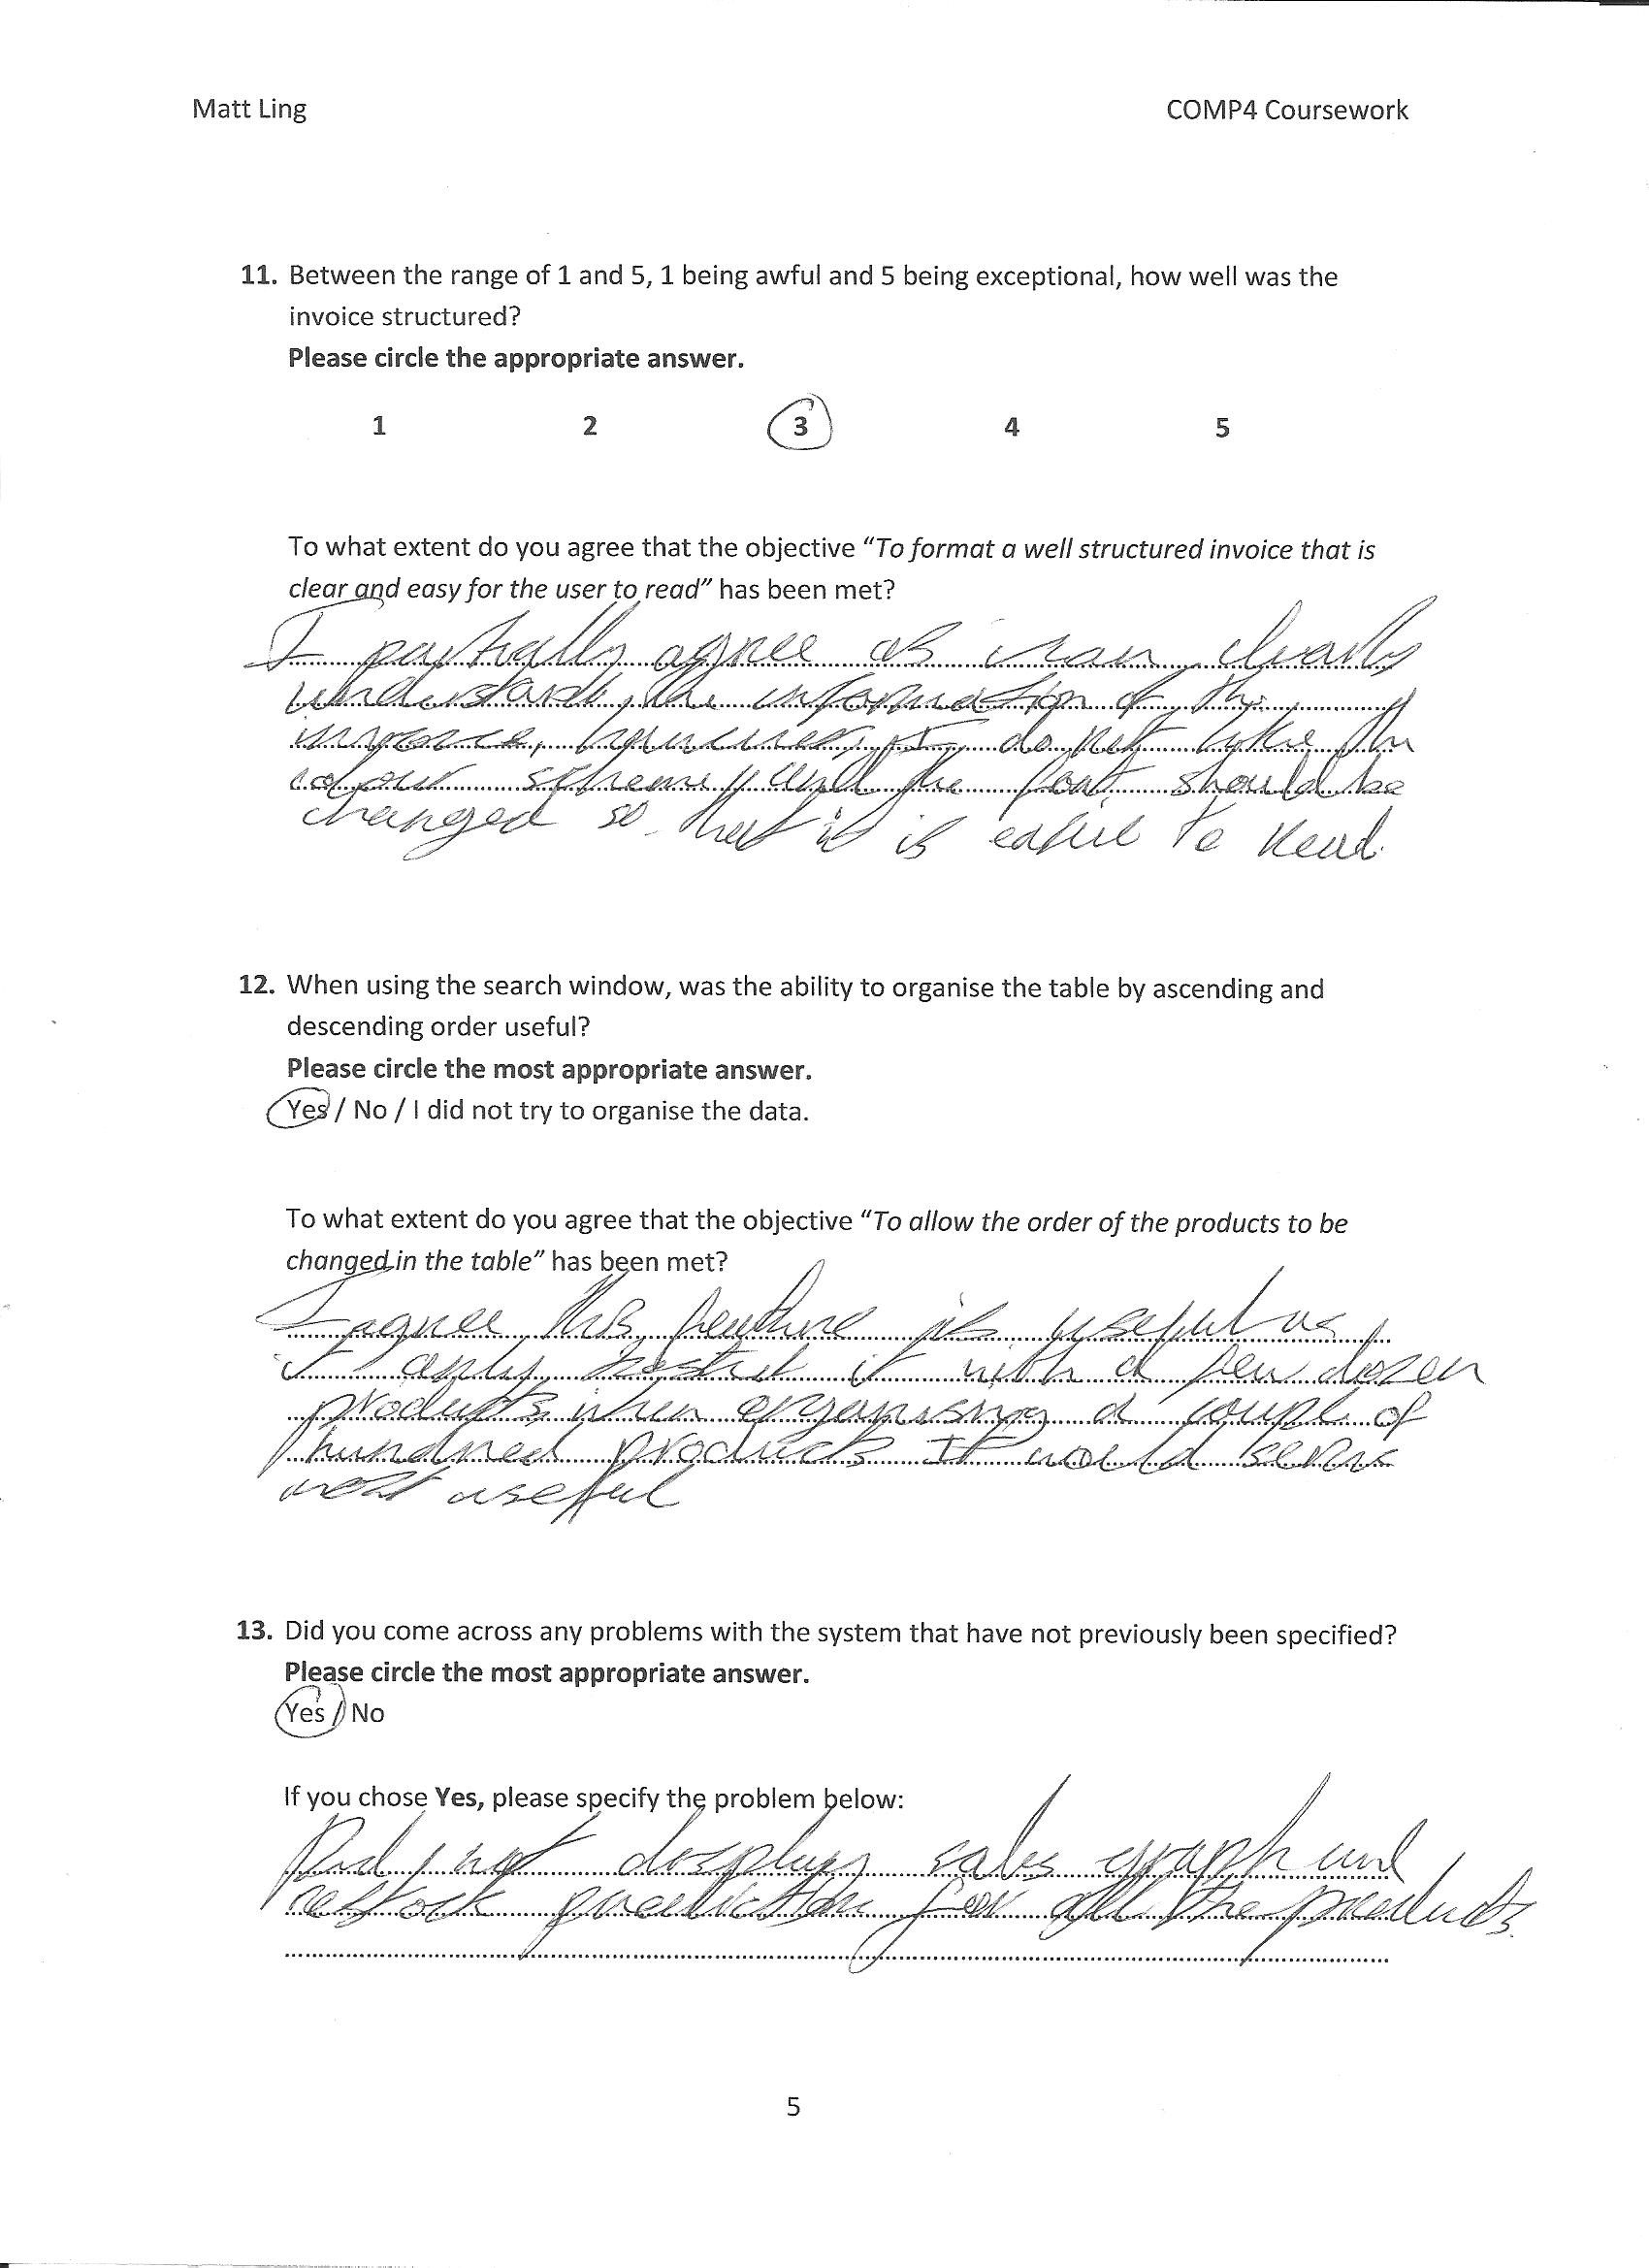
\includepdf{./EvaluationImages/tom-5.jpeg}
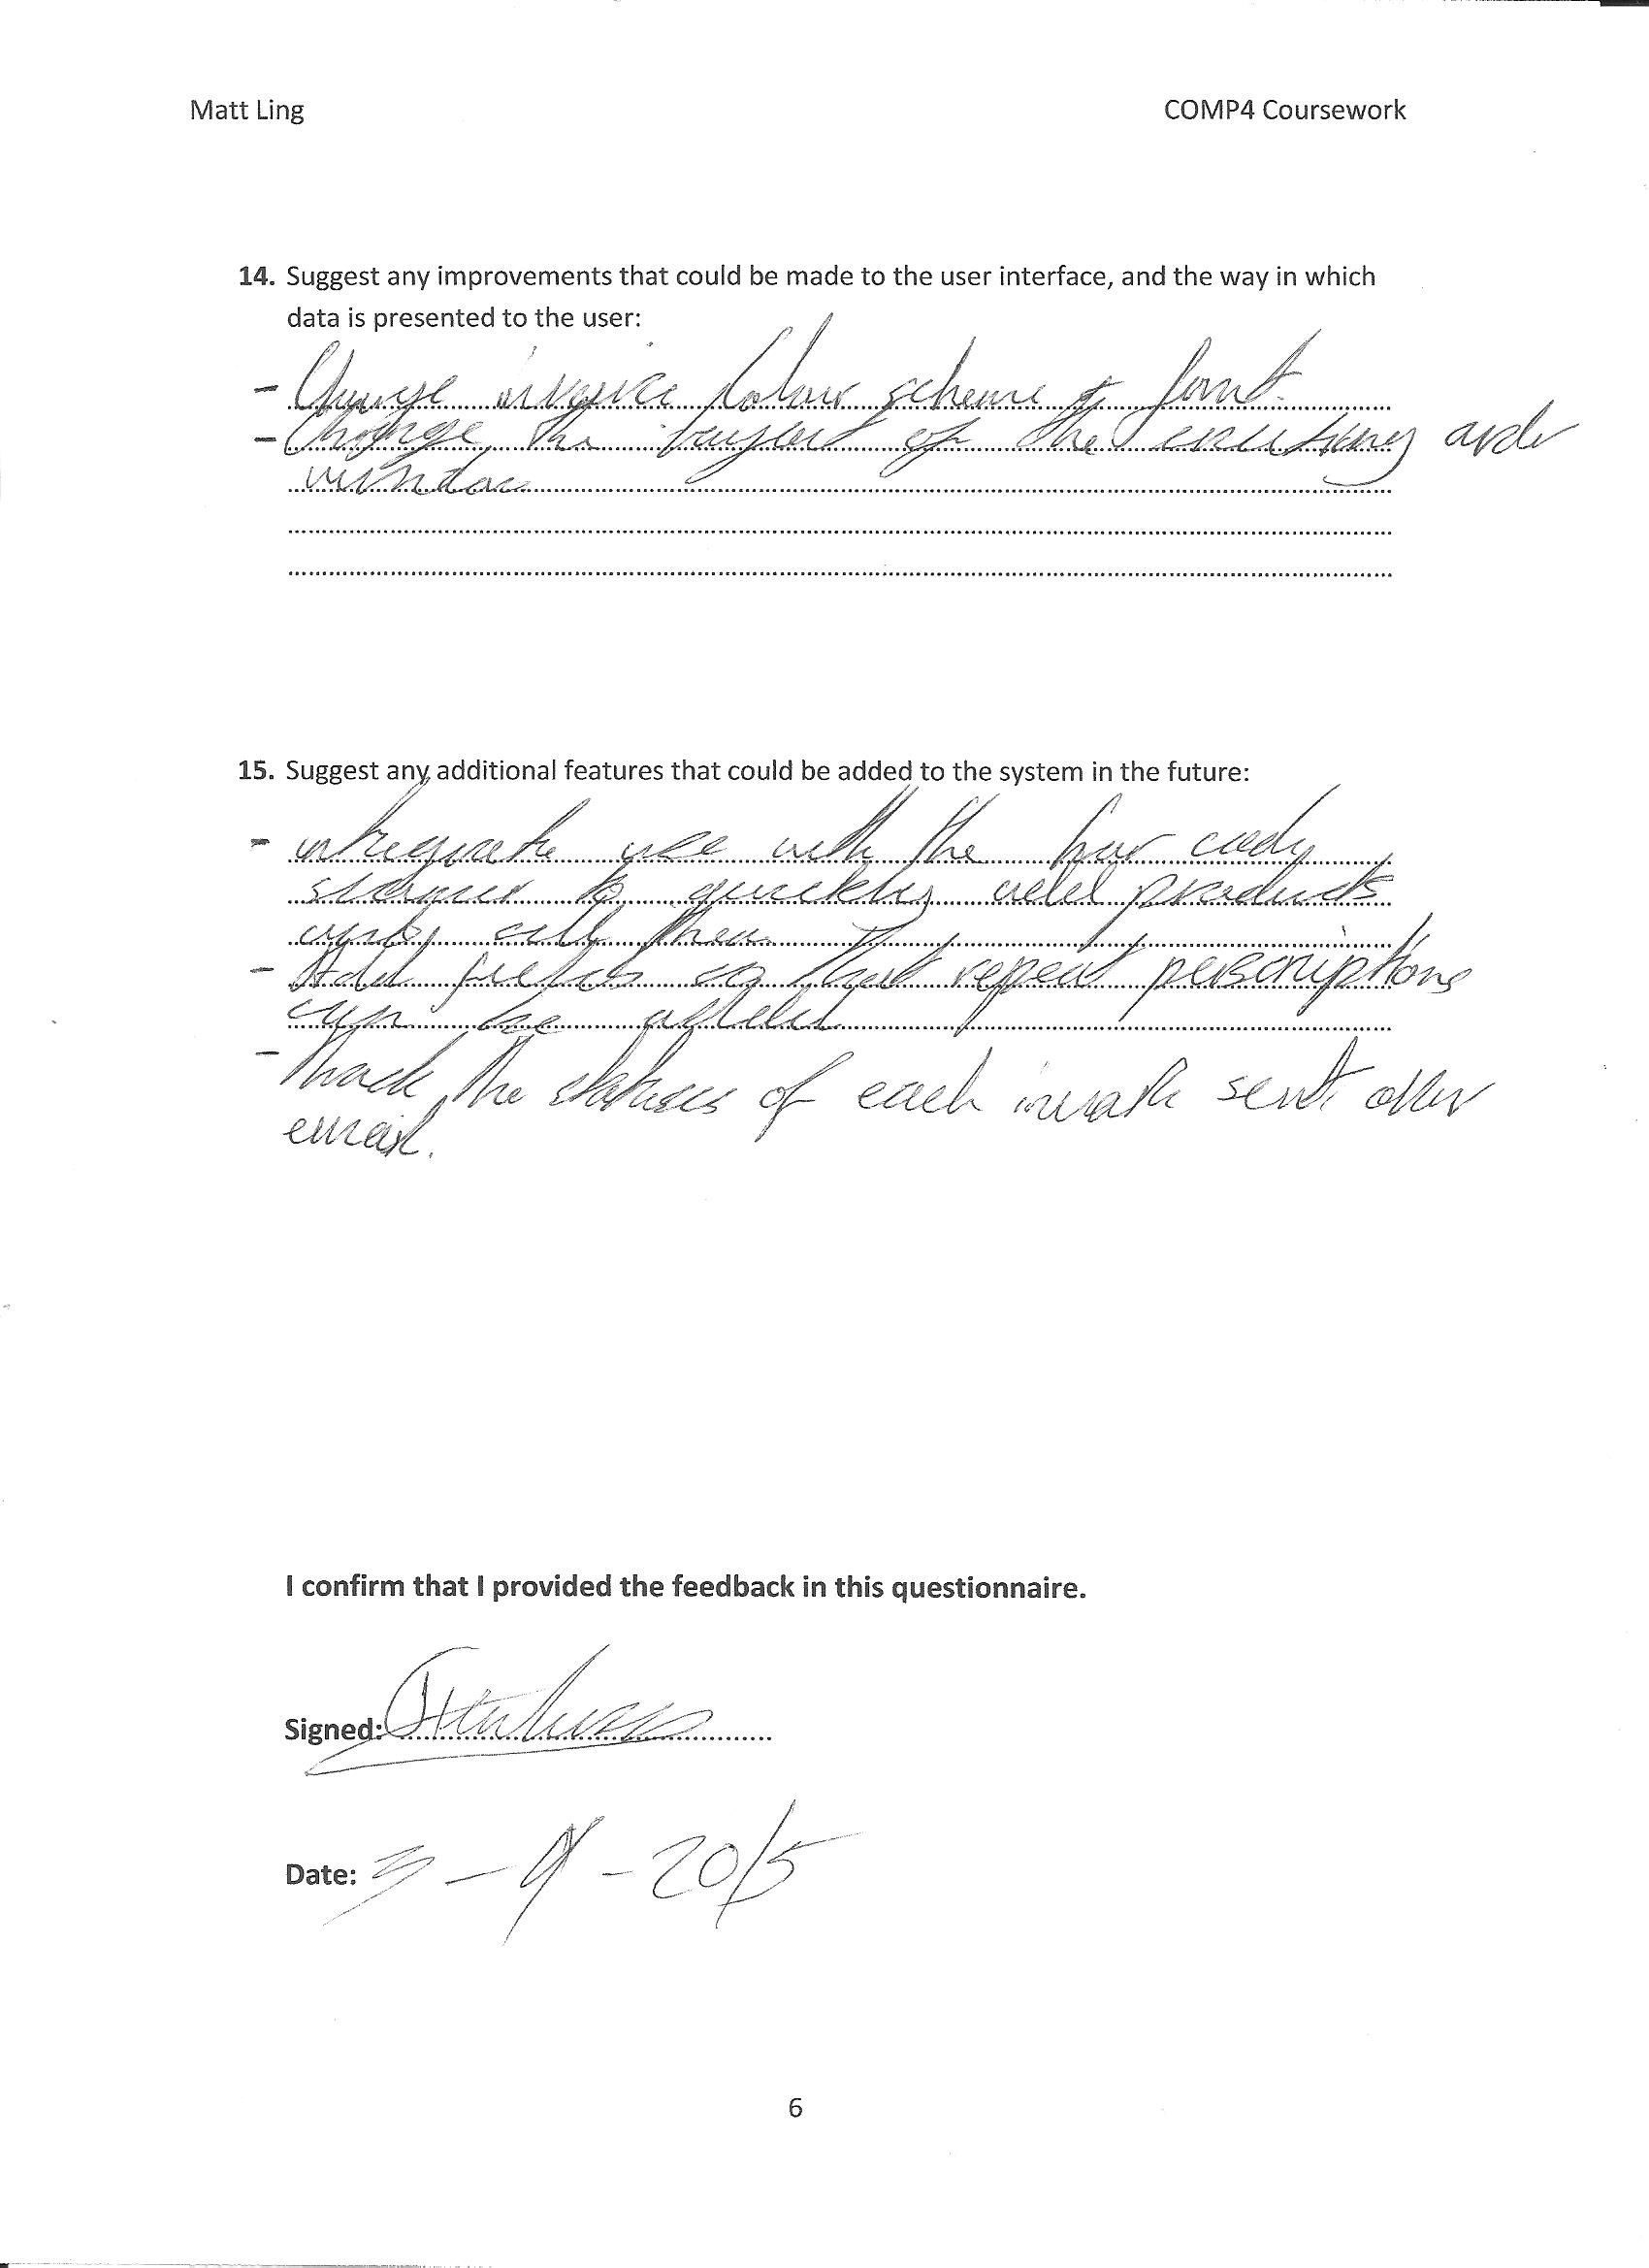
\includepdf{./EvaluationImages/tom-6.jpeg}


\label{Questionnaire2}
\subsubsection{Questionaire 2}
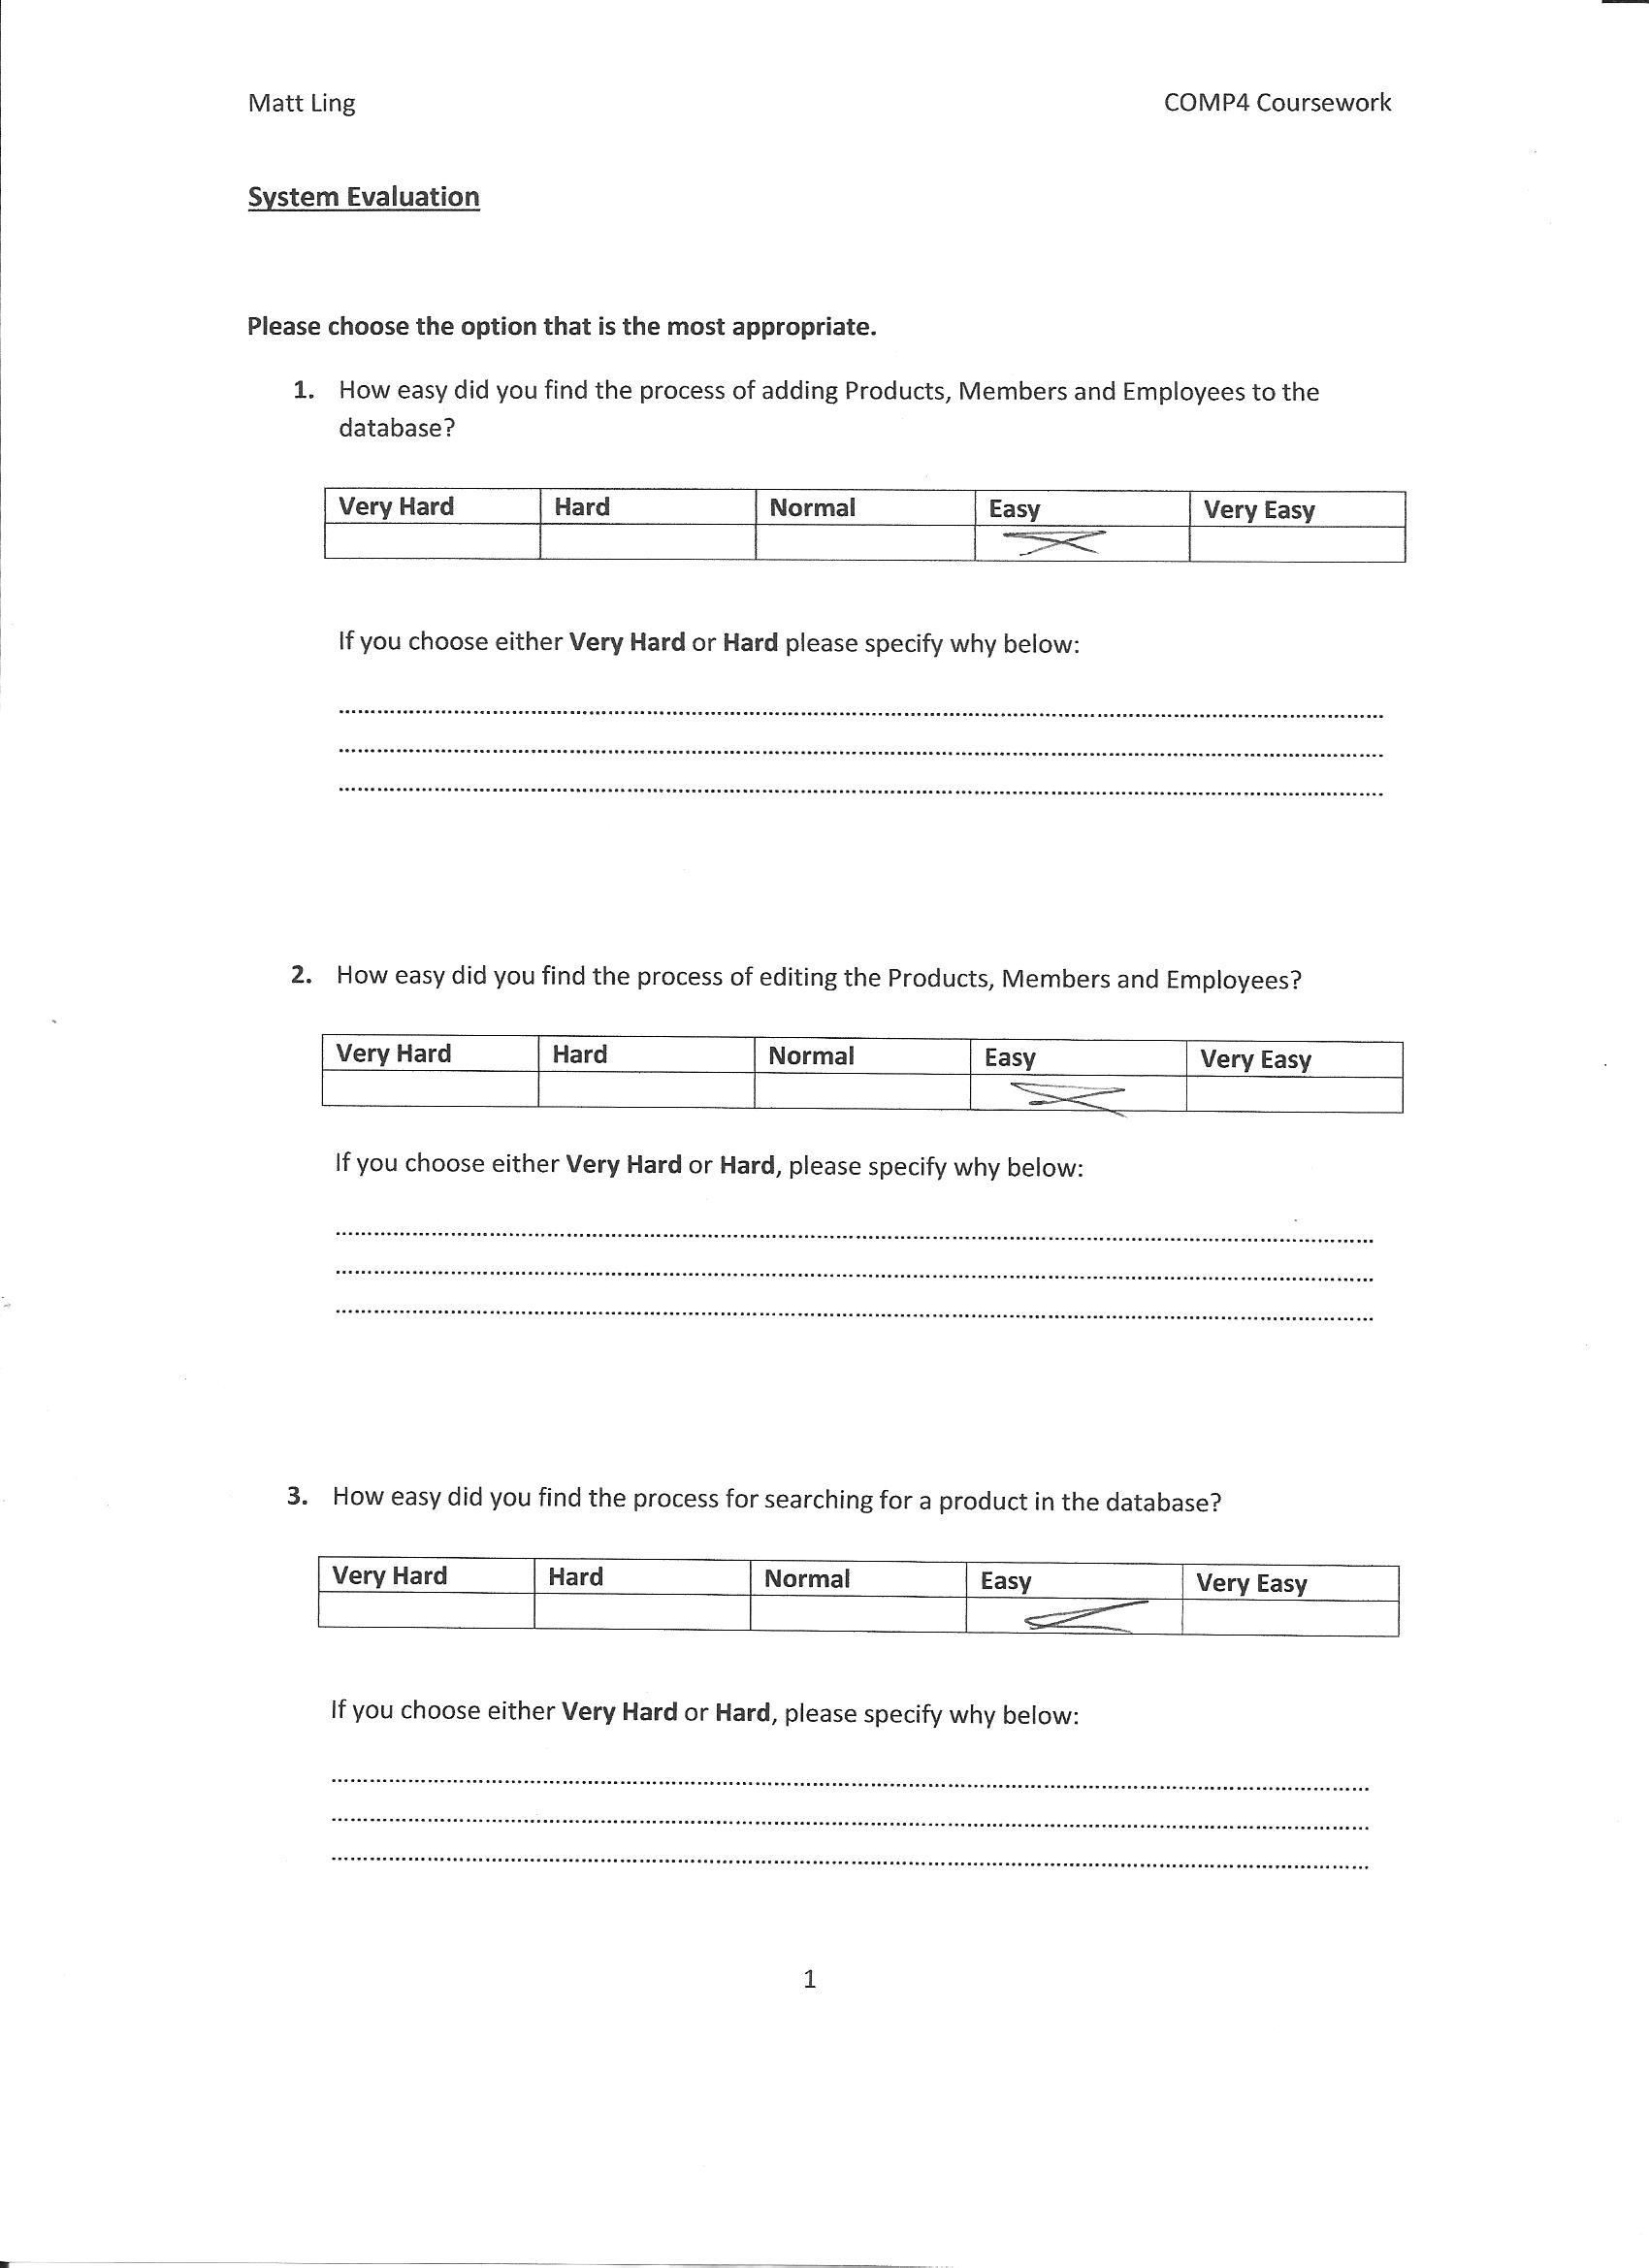
\includepdf{./EvaluationImages/questionaire-1-page-1.jpg}
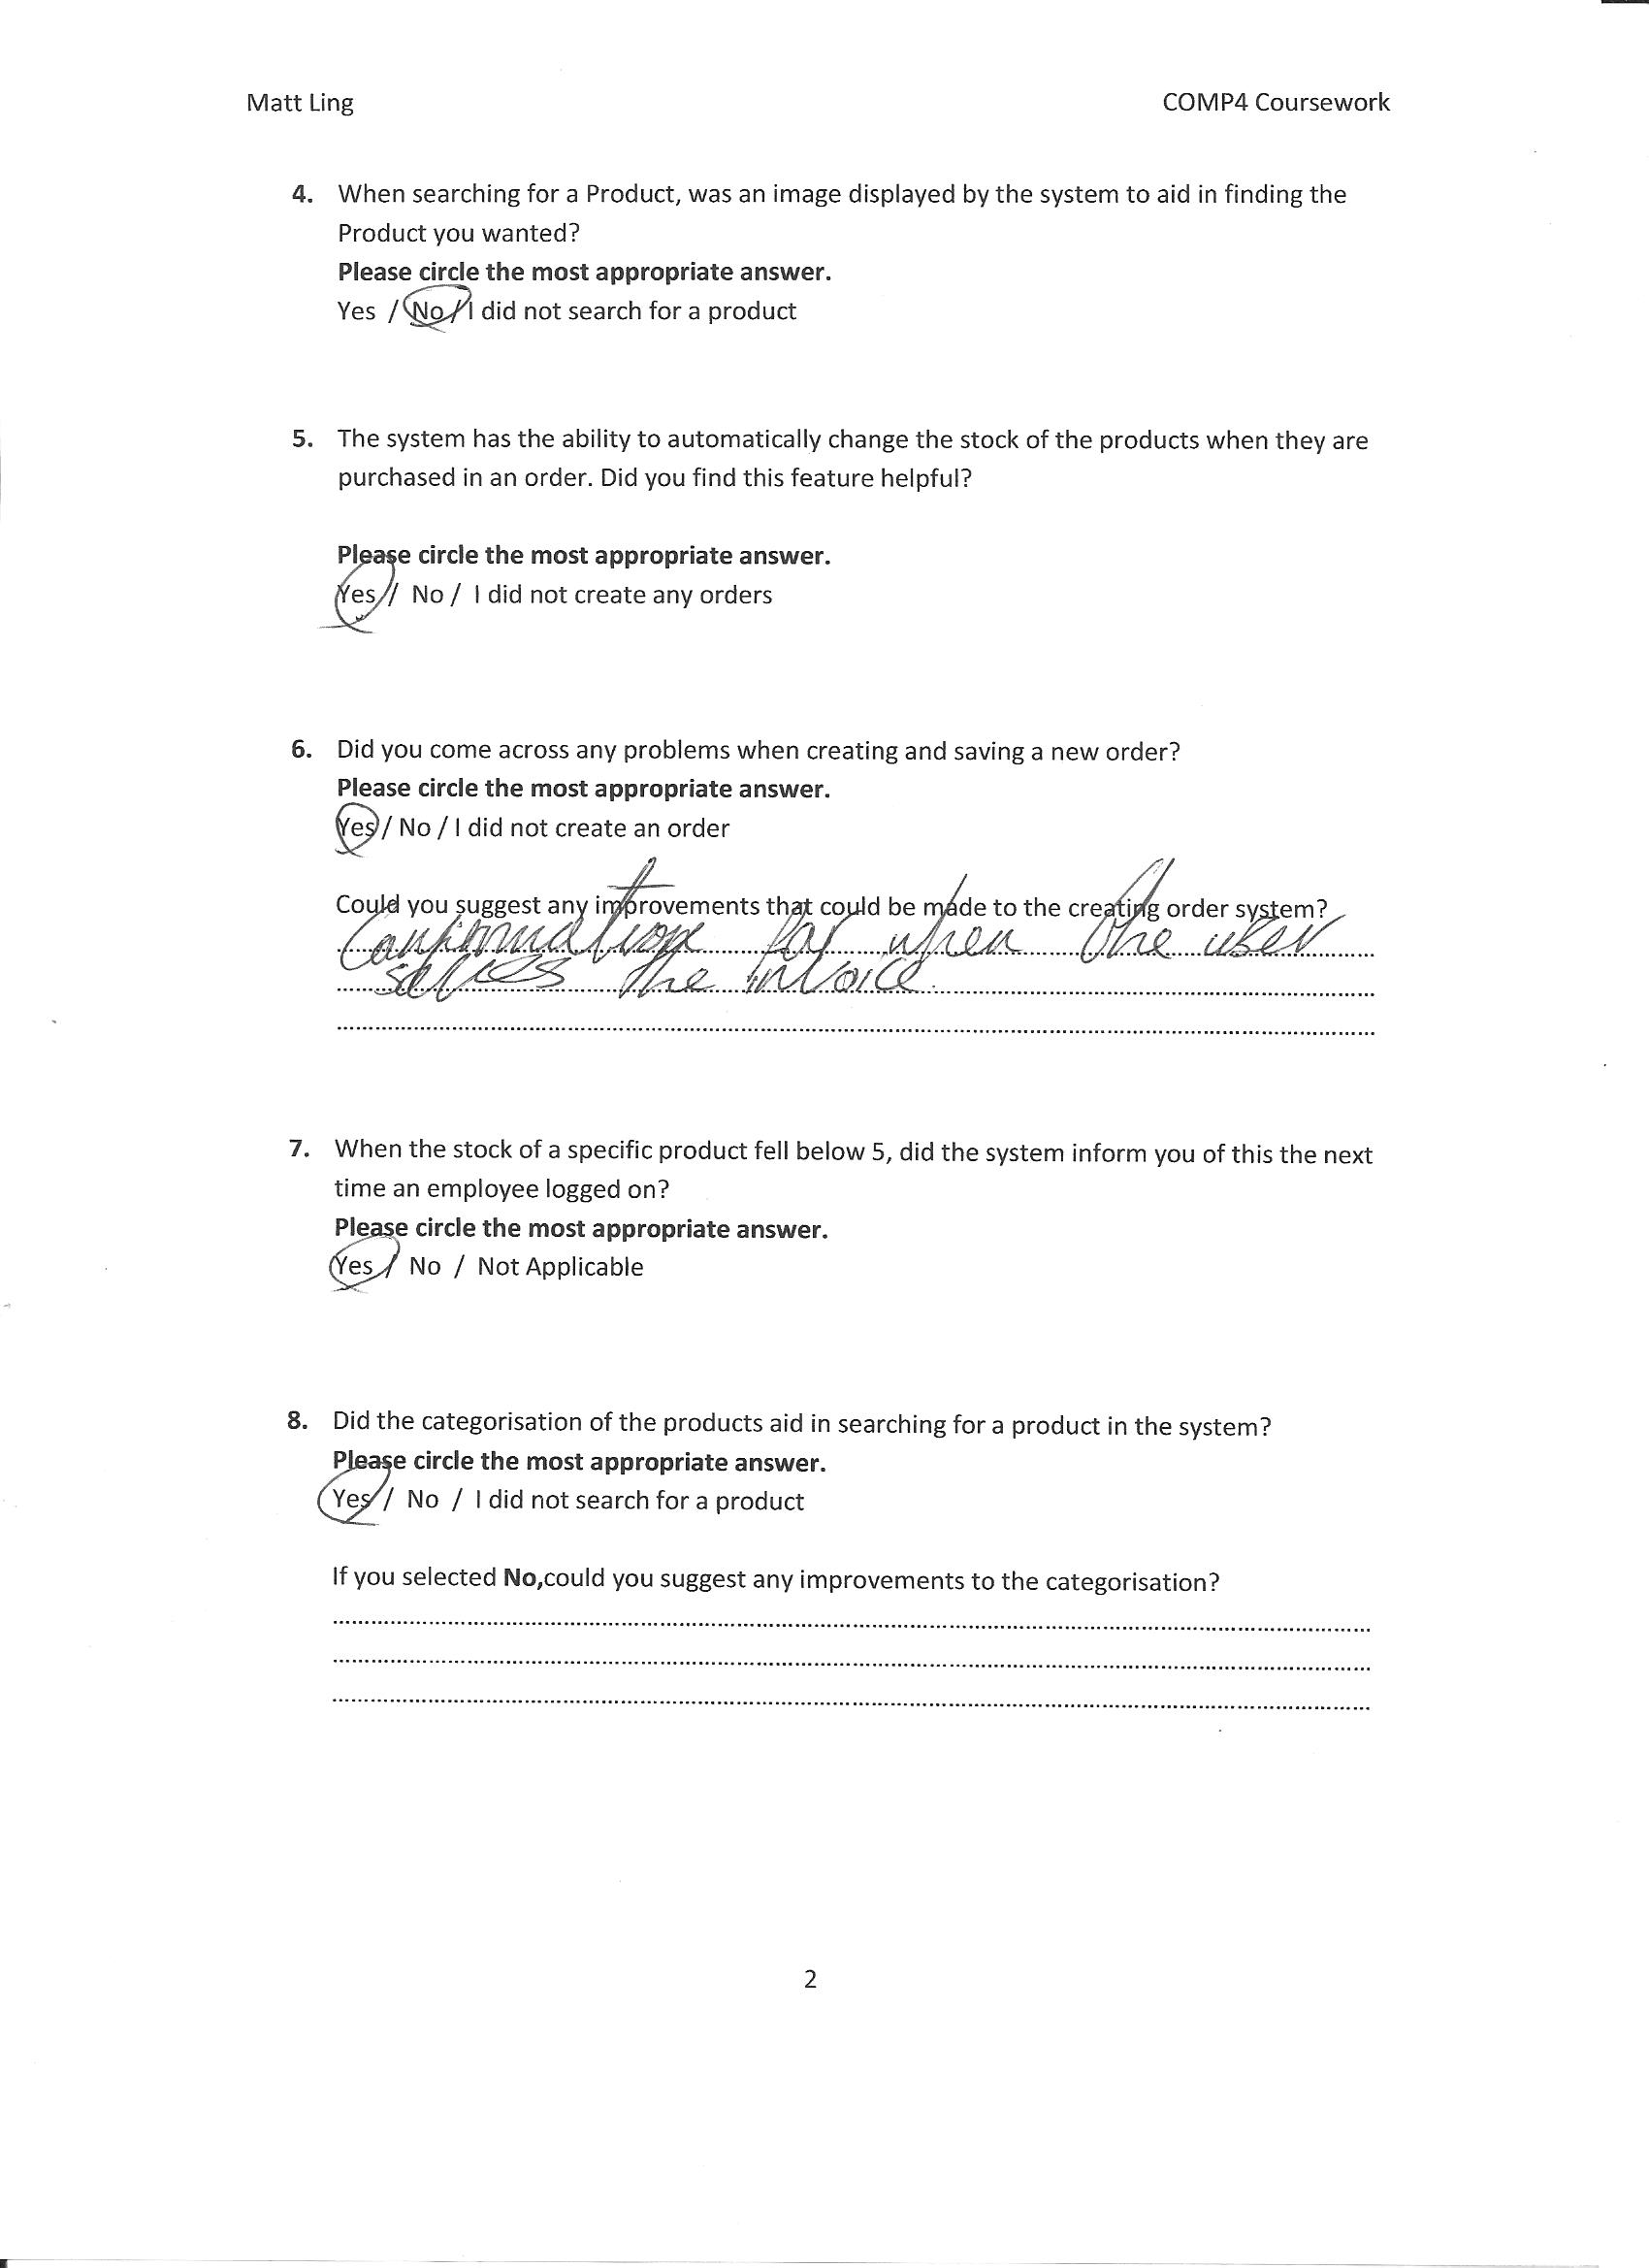
\includepdf{./EvaluationImages/questionaire-1-page-2.jpg}
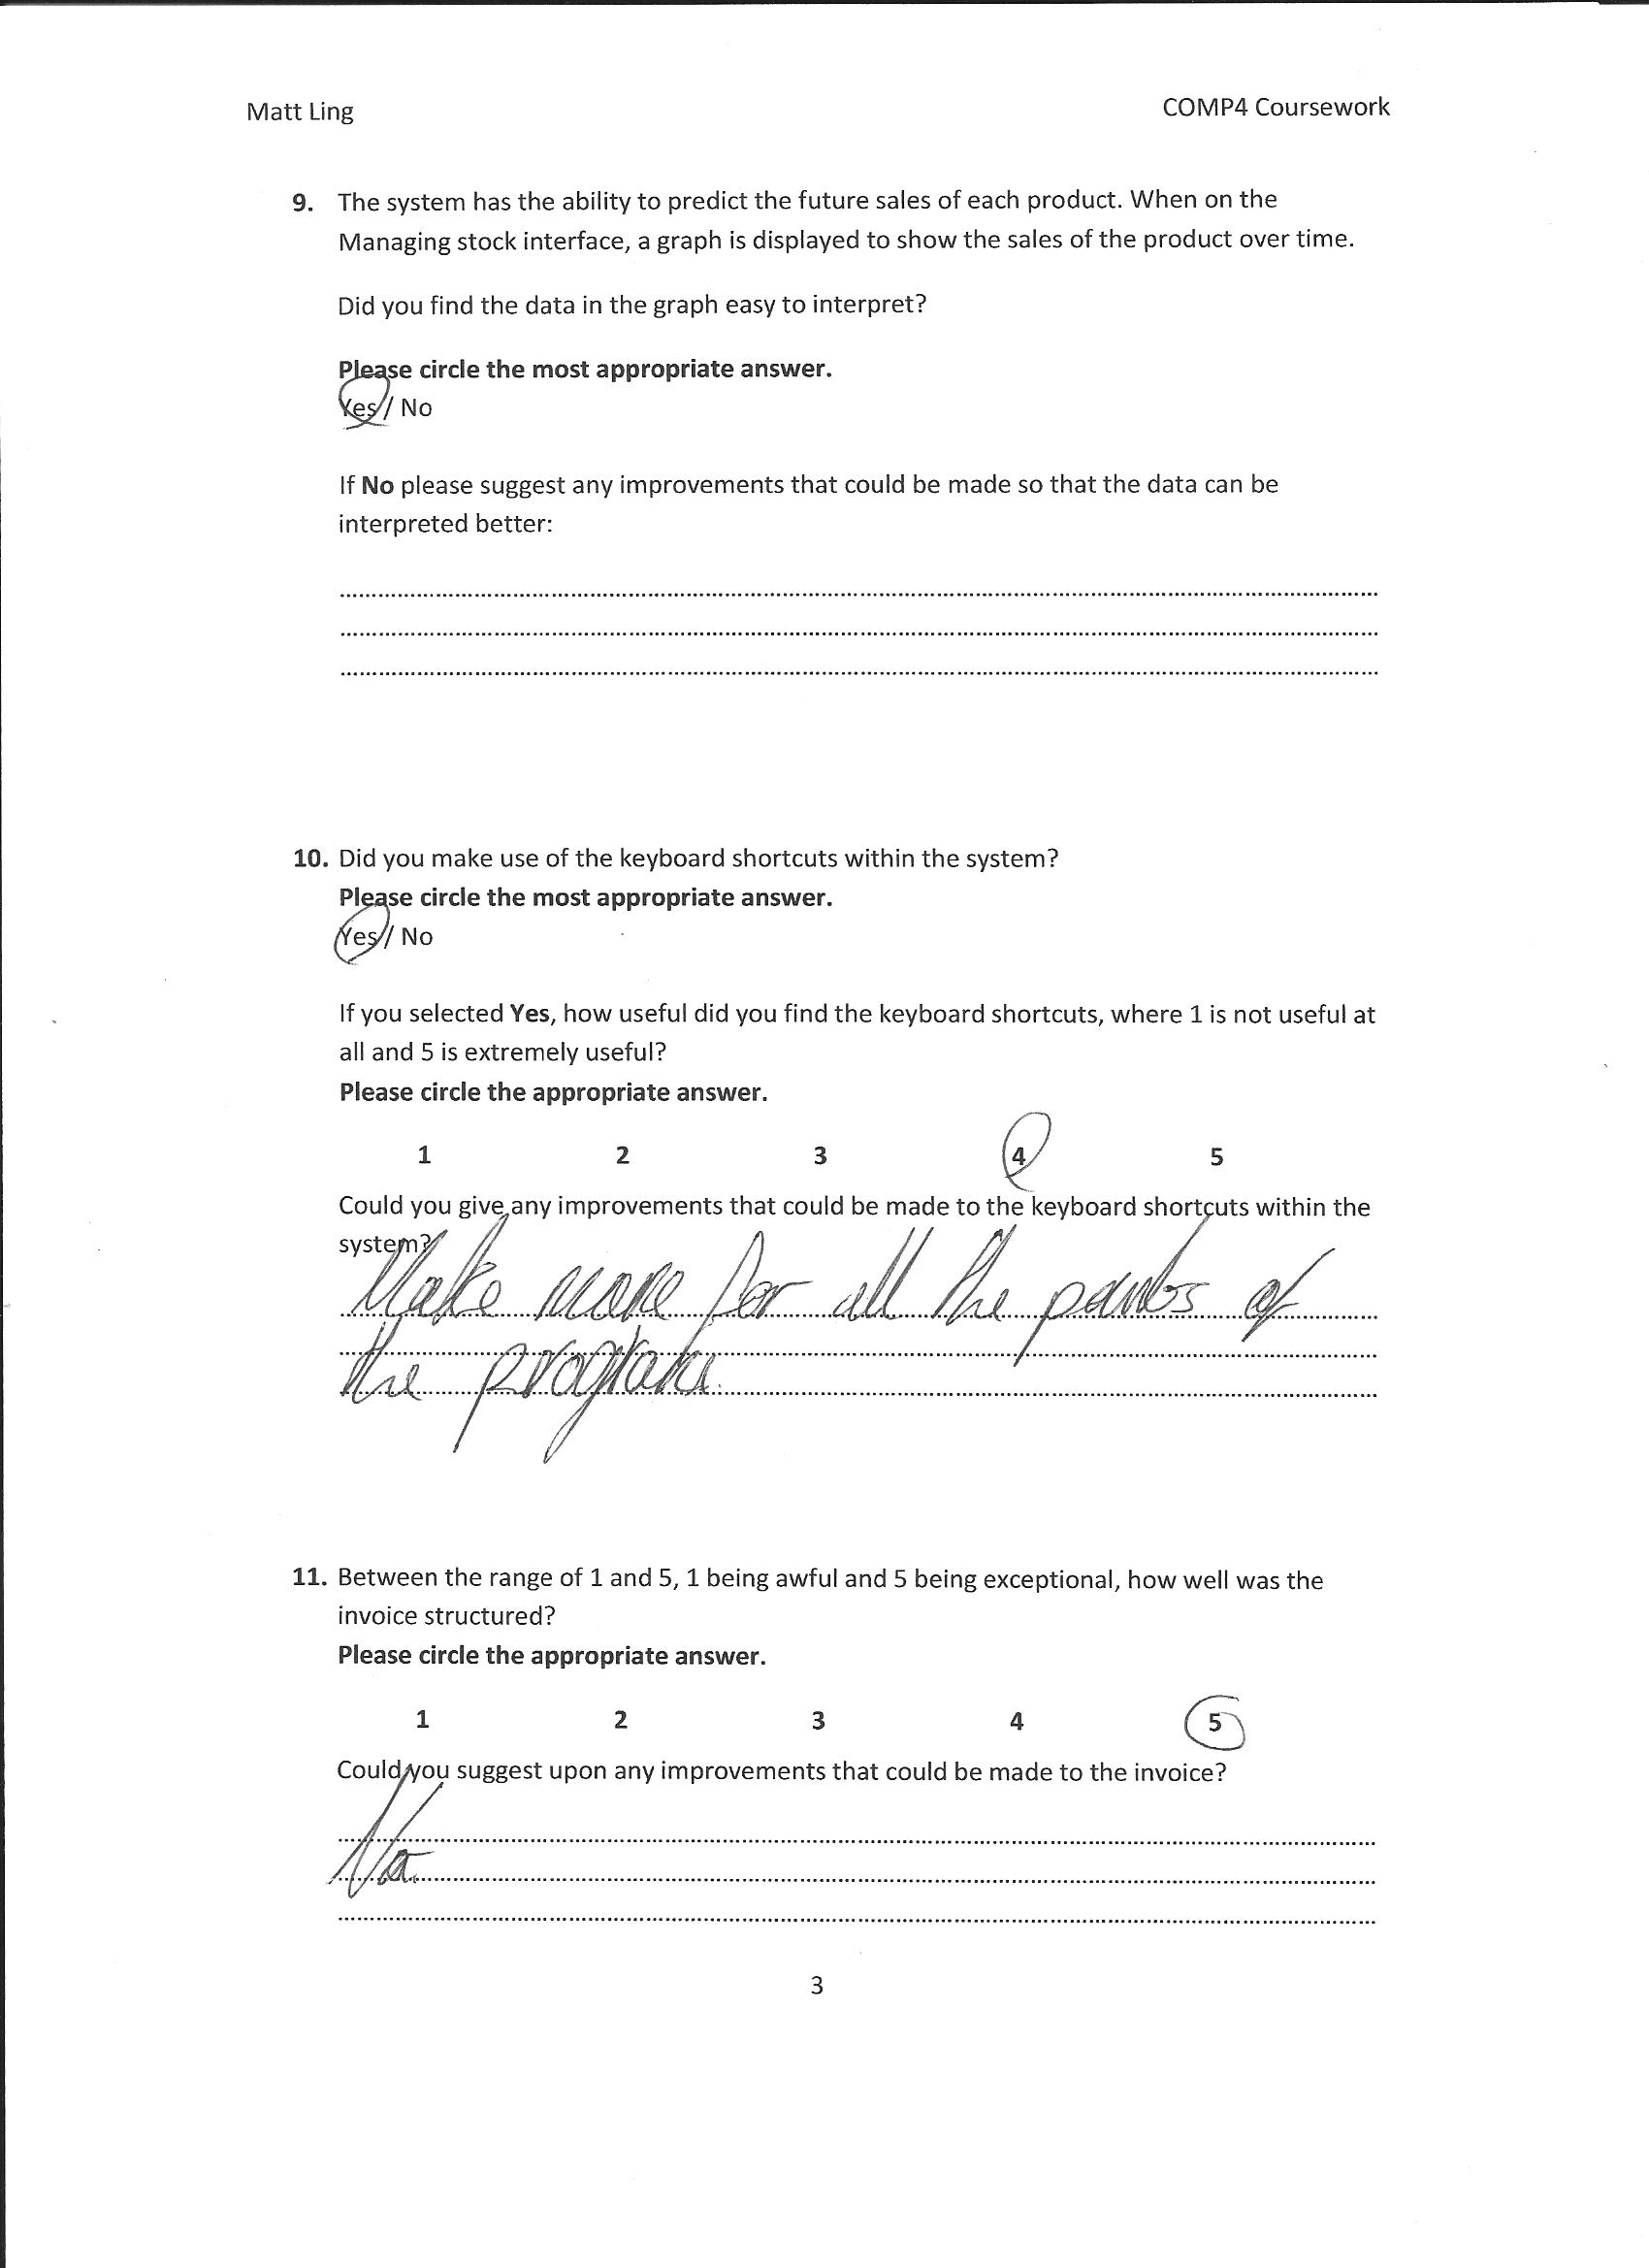
\includepdf{./EvaluationImages/questionaire-1-page-3.jpg}
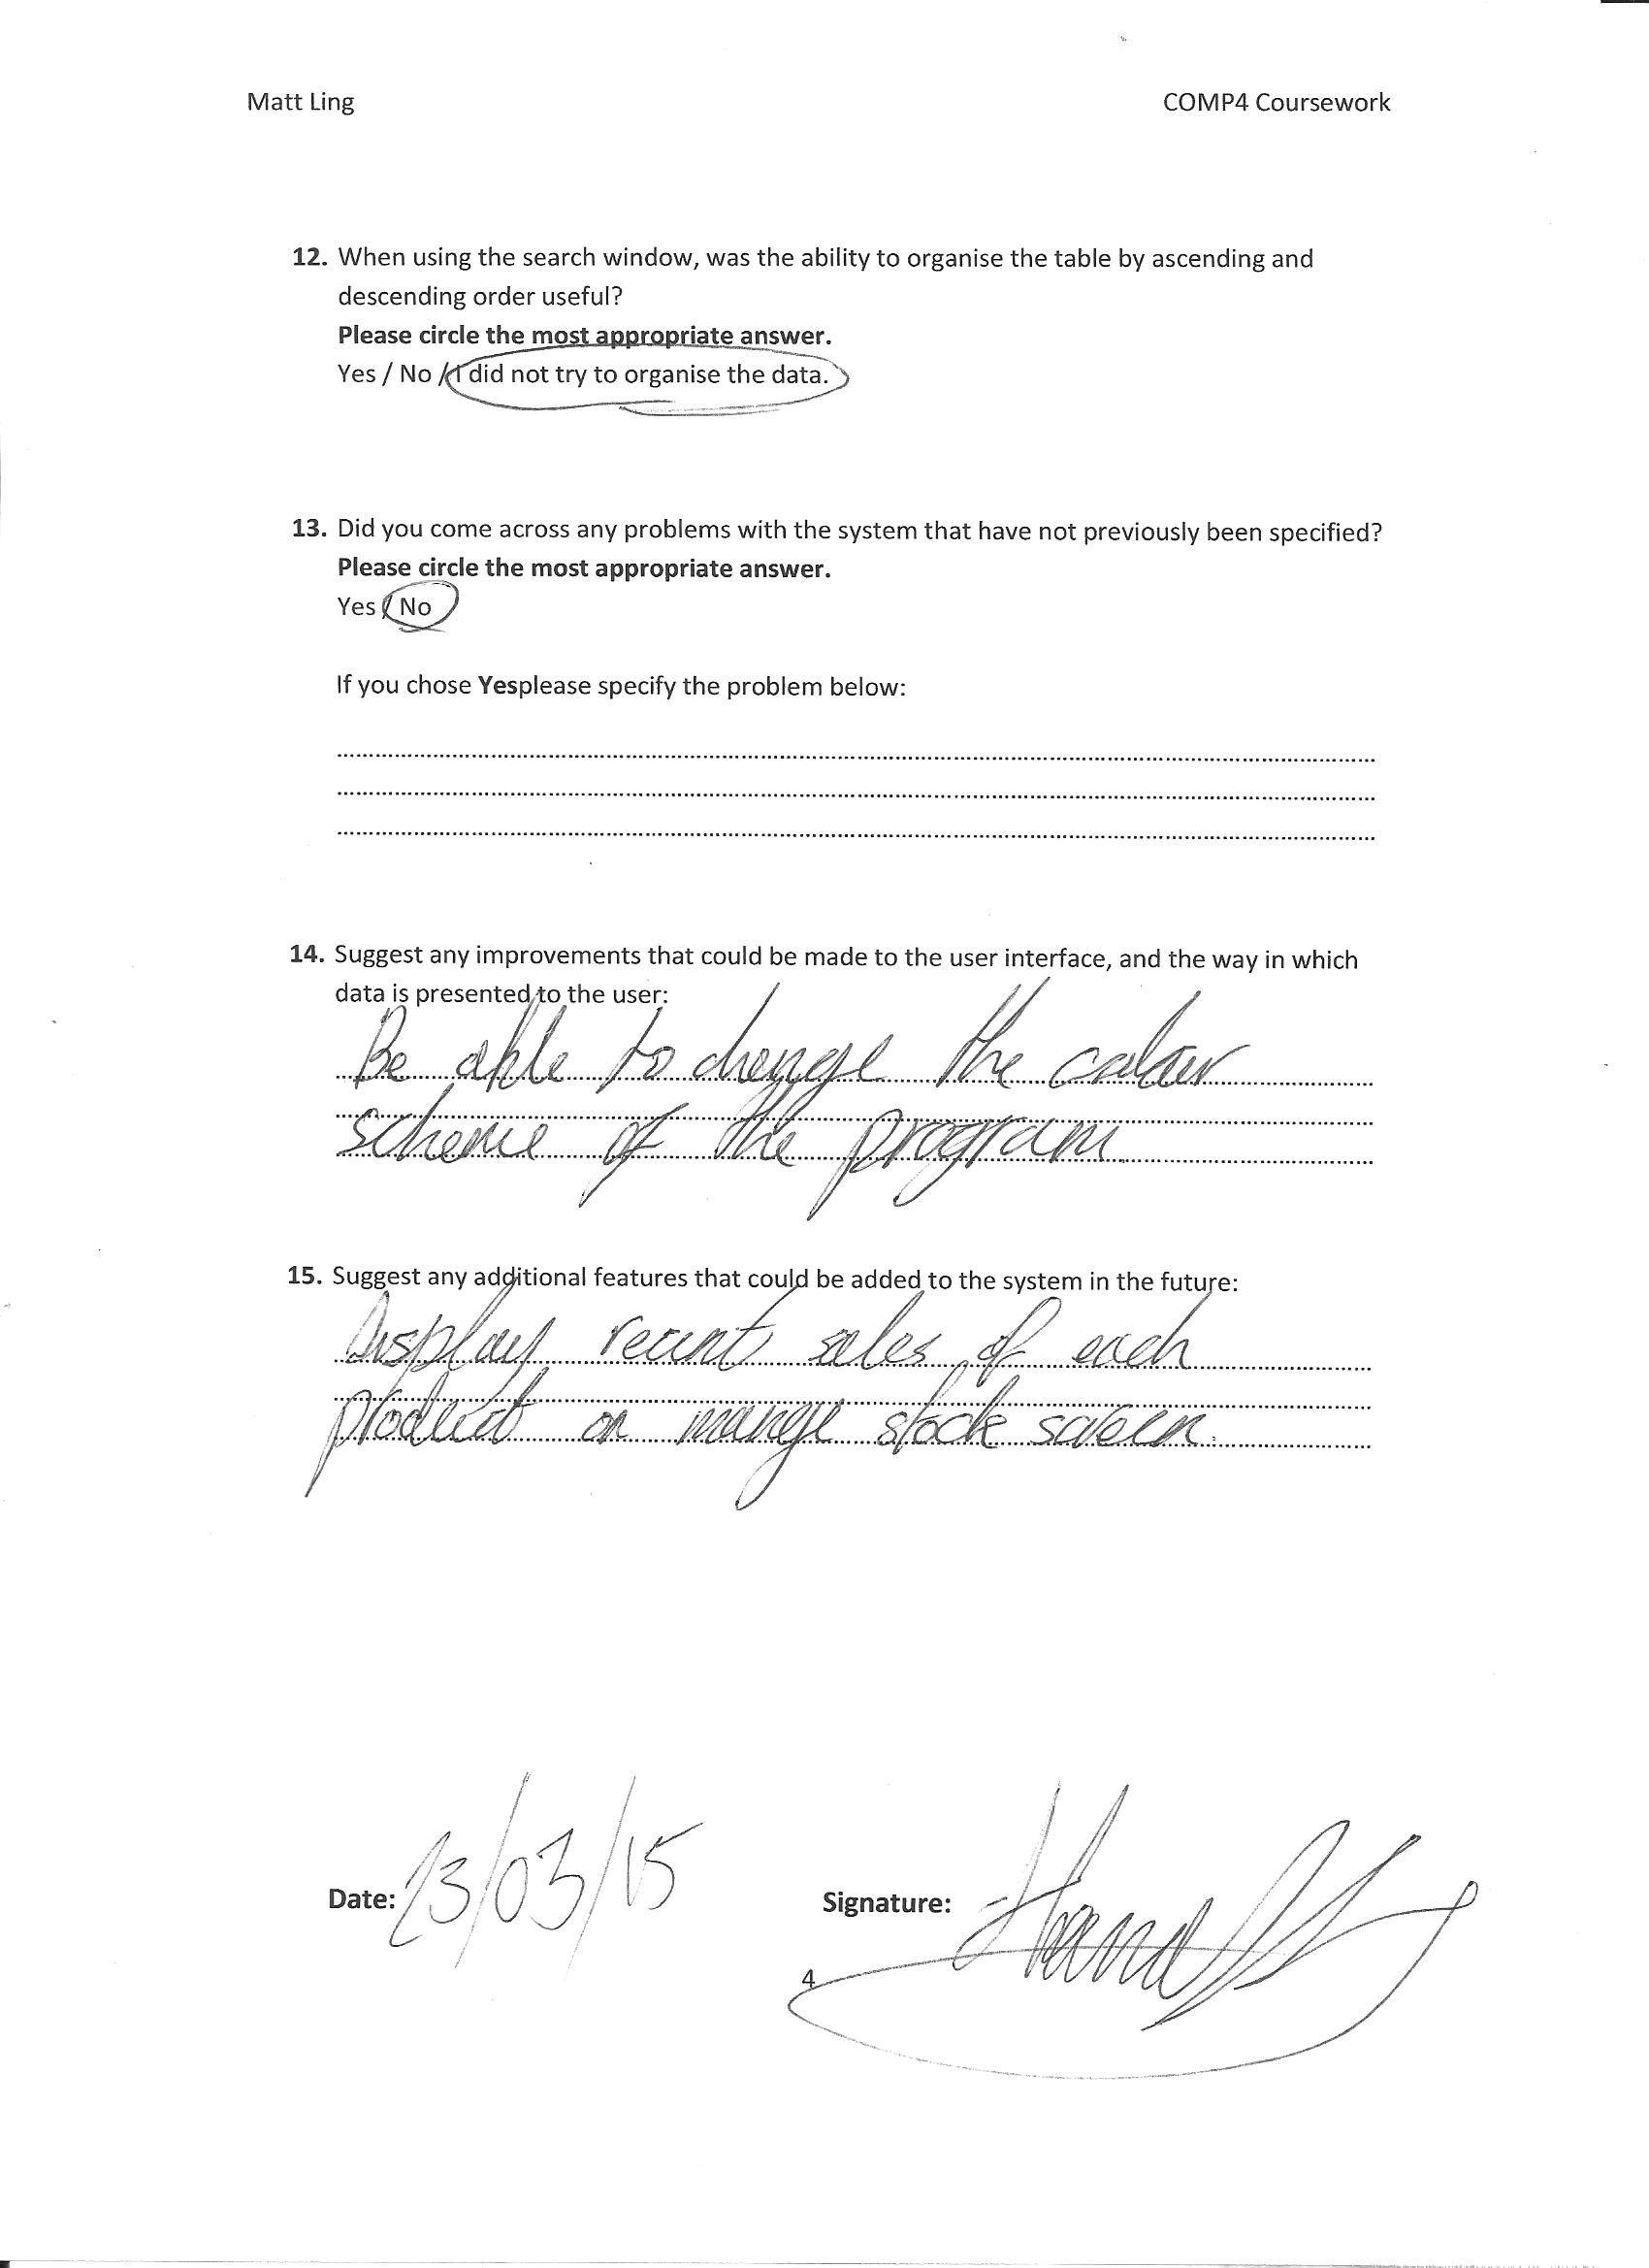
\includepdf{./EvaluationImages/questionaire-1-page-4.jpg}

\label{Questionnaire3}
\subsubsection{Questionaire 3}
\includepdf{./EvaluationImages/questionaire-2-page-1.jpg}
\includepdf{./EvaluationImages/questionaire-2-page-2.jpg}
\includepdf{./EvaluationImages/questionaire-2-page-3.jpg}
\includepdf{./EvaluationImages/questionaire-2-page-4.jpg}

\label{Questionnaire4}
\subsubsection{Questionaire 4}
\includepdf{./EvaluationImages/questionaire-3-page-1.jpg}
\includepdf{./EvaluationImages/questionaire-3-page-2.jpg}
\includepdf{./EvaluationImages/questionaire-3-page-3.jpg}
\includepdf{./EvaluationImages/questionaire-3-page-4.jpg}

\label{Questionnaire5}
\subsubsection{Questionaire 5}
\includepdf{./EvaluationImages/questionaire-4-page-1.jpg}
\includepdf{./EvaluationImages/questionaire-4-page-2.jpg}
\includepdf{./EvaluationImages/questionaire-4-page-3.jpg}
\includepdf{./EvaluationImages/questionaire-4-page-4.jpg}

\label{Questionnaire6}
\subsubsection{Questionaire 6}
\includepdf{./EvaluationImages/questionaire-5-page-1.jpg}
\includepdf{./EvaluationImages/questionaire-5-page-2.jpg}
\includepdf{./EvaluationImages/questionaire-5-page-3.jpg}
\includepdf{./EvaluationImages/questionaire-5-page-4.jpg}

\label{Questionnaire7}
\subsubsection{Questionaire 7}
\includepdf{./EvaluationImages/questionaire-6-page-1.jpg}
\includepdf{./EvaluationImages/questionaire-6-page-2.jpg}
\includepdf{./EvaluationImages/questionaire-6-page-3.jpg}
\includepdf{./EvaluationImages/questionaire-6-page-4.jpg}

\pagebreak
\subsection{Graphs}

\pagebreak
\subsection{Written Statements}

\subsection{Questionnaire 1}

Question 6: ``Confirmation for when the user saves the invoice''

Question 7: ``Make more for all parts of the program''

Question 14: ``Be able to change the colour scheme of the program''

Question 15: ``Display recent sales of each product on manage stock screen''

\subsection{Questionnaire 2}

Question 14: ``Make the green less bright in the colour scheme''

Question 15: ``Be able to track the invoices made. I.e whether they've been paid for or not''

\subsection{Questionnaire 3}

Question 6: ``Make it work with bar code scanner''

Question 11: ``Make invoice text easier to read''

Question 14: ``Use a darker shade of green''

Question 15: ``Not have a log in screen''

\subsection{Questionnaire 4}

Question 6: ``Make the interface larger''

Question 9: ``Stop the dates form overlapping''

Question 11: ``make the text larger''

Question 14: Align text fields on all of the screens''

Question 15: ``intergrate use with the bar code scanner''

\subsection{Questionnaire 5}

Question 10: ''Add more shortcuts to the other screens''

Question 14: ``make the program full screen''

Question 15: ``Know when invoices have been paid for through email''

\subsection{Questionnaire 6}

Question 6: Order Table could be bigger so that more products can be seen.

Question 10: Add more keyboard shortcuts.

Question 11: ``change font size and make it bigger''

Question 14: On the manage stock screen move the stock and name over to the left''

Question 15 ``Be able to see old invoices''


